\documentclass[11pt,twocolumn]{article}
\usepackage[utf8]{inputenc}
\usepackage[T1]{fontenc}
\usepackage{amsmath}
\usepackage{amsfonts}
\usepackage{amssymb}
\usepackage{graphicx}
\usepackage{cite}
\usepackage{url}
\usepackage{hyperref}
\usepackage{algorithm}
\usepackage{algorithmic}
\usepackage{subcaption}
\usepackage{booktabs}
\usepackage{geometry}
\usepackage{fancyhdr}
\usepackage{times}
\usepackage{balance}
\usepackage{xcolor}
\usepackage{tabularx}
\usepackage{listings}
\geometry{margin=0.75in}
\usepackage[section]{placeins}
\usepackage{stfloats}
\usepackage{pgfplots}
\usepackage{pgfplotstable}
\pgfplotsset{compat=1.18}
\setlength{\textfloatsep}{6pt plus 2pt minus 2pt}
\setlength{\intextsep}{6pt plus 2pt minus 2pt}
\hypersetup{hidelinks}

\lstset{
    basicstyle=\footnotesize\ttfamily,
    breaklines=true,
    frame=single,
    captionpos=b,
    numbers=left,
    numberstyle=\tiny,
    showstringspaces=false,
    language=C
}

\lstdefinelanguage{JavaScript}{
  keywords={typeof, new, true, false, catch, function, return, null, catch, switch, var, if, in, while, do, else, case, break, const, let, class, export, import, async, await},
  keywordstyle=\color{blue}\bfseries,
  ndkeywords={class, export, boolean, throw, implements, import, this},
  ndkeywordstyle=\color{darkgray}\bfseries,
  identifierstyle=\color{black},
  sensitive=false,
  comment=[l]{//},
  morecomment=[s]{/*}{*/},
  commentstyle=\color{purple}\ttfamily,
  stringstyle=\color{red}\ttfamily,
  morestring=[b]',
  morestring=[b]"
}

\pagestyle{fancy}
\fancyhf{}
\fancyhead[L]{\scriptsize AWARE: Smart Caching for Emergency Flood Warnings}
\fancyhead[R]{\scriptsize \thepage}
\renewcommand{\headrulewidth}{0.4pt}

\title{\Large\textbf{Smart Caching and Offline Emergency Warning Systems for Flood Scenarios: AWARE EAS Framework}}

\author{
    \textbf{Charles Melvin}\textsuperscript{1}, \textbf{N. Rich Nguyen}\textsuperscript{2} \\
    \small\textsuperscript{1}Department of Computer Science, University of Virginia, Charlottesville, VA 22903 \\
    \small\texttt{\{jgm6jy, nn4pj\}@virginia.edu}
}

\date{\small Submitted: TBD}

\begin{document}

\maketitle

\begin{abstract}
\noindent AWARE is a client-side framework for smart caching and resilient delivery of flood emergency alerts that explicitly optimizes what to push and what to cache when connectivity is fragile. The design couples a semantic eviction policy (PriorityFresh) with a lightweight probabilistic Priority Forecasting (PF) model that learns how severity, urgency, freshness, and region context map to user-relevant value. The PF model leverages regional anomaly history to adapt priorities to local patterns (e.g., regions where severe warnings often divert at the last minute). The simulator renders seeded environments, synthesizes alert streams, and evaluates cache policies and push strategies under rate limits and deduplication. Offline metrics jointly reflect system efficiency (delivery rate, hit rate) and human-centered outcomes (freshness, redundancy, actionability-first, timeliness consistency), enabling head-to-head comparisons of PriorityFresh against frequency-driven TinyLFU admission. The framework outlines a path toward adaptive, offline-first warning systems where the decision to push is learned from outcomes rather than hard-coded thresholds.
\end{abstract}

\noindent\textbf{Keywords:} 
Emergency Alert System, Flood Warning, Floodwatch, Offline Caching, 
Smart Cities, Disaster Management, Edge Computing, Dexie, 
Progressive Web Applications, Offline-First Applications, 
Delay-Tolerant Networking (DTN), Mesh Networking, 
Local-First Software, Service Workers, 
Disaster Communication, Crisis Informatics, 
Human-Centered Computing, Cognitive Load, 
Stress-Aware Design, Resilient Networking

\vspace{0.3cm}

\section{Introduction and Research Question}
Disaster-time information systems face a simple but consequential question: \emph{How can we most effectively deliver the most pressing matters to people?} In AWARE, we treat “most pressing” as alerts that are both \emph{high-impact} (severity, urgency) and \emph{still relevant} (freshness). PriorityFresh operationalizes this by ranking content semantically and maintaining top-priority items until they decay below relevance or expire. The PF (Priority Forecasting) model can further bias toward items historically most valuable in a region, subject to rate limits and deduplication to avoid overwhelming users.

\section{Smart Caching Algorithm}
AWARE ships the cache policies that are currently implemented in \texttt{src/sim/policies}.

\subsection{Policies available}
\begin{itemize}
    \item \textbf{LRU} evicts the least recently accessed alert after purging expired entries.
    \item \textbf{TTLOnly} keeps alerts until they expire, without considering recency.
    \item \textbf{PriorityFresh} scores alerts by semantic priority and freshness before eviction.
    \item \textbf{PAFTinyLFU} combines recency with a TinyLFU frequency sketch to admit only likely high-utility alerts.
\end{itemize}

\subsection{PriorityFresh scoring}
The PriorityFresh policy maintains an in-memory map with capacity $C$ and assigns each alert $a$ the base score
$$
\mathrm{base}(a,t) = w_S \, s(a) + w_U \, u(a) + w_F \, f(a,t),
$$
where $s(a)$ and $u(a)$ are ordinal encodings (in code: $s(\text{Minor}){=}1,\ s(\text{Moderate}){=}2,\ s(\text{Severe}){=}3,\ s(\text{Extreme}){=}4,\ s(\text{Unknown}){\approx}2$ and $u(\text{Past}){=}0.5,\ u(\text{Future}){=}1.5,\ u(\text{Expected}){=}2,\ u(\text{Immediate}){=}3,\ u(\text{Unknown}){\approx}1.5$), and $f(a,t) = e^{-\lambda (t - a_{\text{issued}})}$ applies exponential decay with $\lambda = 1/600$. Default weights emphasise urgency over severity: $w_S{=}2$, $w_U{=}3$, $w_F{=}4$; operators can adjust them per run. When the cache is full, the alert with the lowest total score is evicted before inserting the newcomer. Expired alerts are purged on every read and write.
For query-side retrieval, the simulator samples cached items with an urgency-first bias.

PriorityFresh can integrate a learned PF-based boost to obtain a total score
$$
\mathrm{total}(a,t) = \mathrm{base}(a,t) + \underbrace{\Delta(a,t)}_{\text{PF boost}},
$$
where the boost $\Delta(a,t)$ is proportional to the model's estimated probability of high utility for the user and may include controlled exploration during training.

\subsection{Push notification optimization}
\label{sec:push-optimization}
Push delivery is modeled as a decision at alert arrival time under two operational constraints: a rate limit $R$ pushes per minute and a deduplication window $D$ seconds that suppresses rapid repeats from the same \emph{thread}. Given alert $a$ at time $t$, PriorityFresh supplies $\mathrm{base}(a,t)$ and PF supplies a probability $p(a,t) \in [0,1]$ that the alert will be valuable if surfaced now. A push occurs if all of the following hold:
\begin{enumerate}
        \item within the rate limit (fewer than $R$ pushes in the last 60 seconds),
        \item not a recent duplicate (no push for the same \texttt{threadKey} within $D$ seconds), and
        \item $p(a,t) \ge \tau$ or $a$ is high-impact (\emph{Extreme} or \emph{Immediate}).
\end{enumerate}
The threshold $\tau$ is configurable; during training, $\epsilon$-greedy exploration with probability $\epsilon$ occasionally pushes borderline cases to learn from outcomes. The simulator tracks pushes sent, suppressions (by reason), duplicate rates, and first-push timeliness per thread.

\begin{algorithm}[t]
\caption{PriorityFresh+PF: cache and push on arrival}
\label{alg:pf-priorityfresh}
\begin{algorithmic}[1]
\REQUIRE capacity $C$, weights $w_S,w_U,w_F$, rate limit $R$/min, dedup window $D$, PF model $\mathcal{M}$
\STATE purgeExpired($t$)
\STATE base $\leftarrow w_S s(a)+ w_U u(a)+ w_F f(a,t)$
\STATE $p \leftarrow \mathcal{M}.\text{predict}(a, t, \text{freshness}=f(a,t), \text{base})$
\STATE total $\leftarrow$ base $+ \Delta(p,\text{explore})$
\IF{cache is full} \STATE evict min-score entry \ENDIF
\STATE insert $a$ with score total
\IF{within rate limit AND not duplicate AND $(p \ge \tau$ OR high-impact$)$}
    \STATE send push; record timestamp and thread
\ELSE
    \STATE suppress push; record suppression reason
\ENDIF
\end{algorithmic}
\end{algorithm}

\section{Experimental Setup (No Results)}
This section documents the experimental configuration and visual assets that summarize the test runs. We deliberately avoid interpreting outcomes here.

\subsection{Default parameters}
Unless otherwise specified, all single-seed comparisons use the following settings:

\begin{table}[h]
\centering
\caption{Default run configuration}
\label{tab:default-config}
\begin{tabular}{@{}ll@{}}
    \toprule
Scenario & Urban \\
Cache Size & 128 \\
Alerts & 400 \\
Severity weight $w_S$ & 4 \\
Urgency weight $w_U$ & 5 \\
Freshness weight $w_F$ & 5 \\
Network reliability & 0.85 \\
Seed & FISHDINNER \\
Seed mode & fixed (single seed) \\
Replicates & 1 \\
Duration (sec) & 900 \\
Query rate (per minute) & 60 \\
\bottomrule
\end{tabular}
\end{table}

\noindent PF (Priority Forecasting) model settings used throughout (held constant):

\begin{table}[h]
\centering
\caption{PF model settings (constant)}
\label{tab:pf-settings}
\begin{tabular}{@{}ll@{}}
    \toprule
Rate limit & 0 \\
Dedup window (sec) & 120 \\
PF threshold $\tau$ & 0.5 \\
Exploration $\epsilon$ & 0.05 \\
\bottomrule
\end{tabular}
\end{table}

\noindent Delivery behavior for single-seed (non-randomized) runs:

\begin{table}[h]
\centering
\caption{Delivery settings (single-seed runs only)}
\label{tab:delivery-settings}
\begin{tabular}{@{}ll@{}}
   \toprule
Retry interval (sec) & 1 \\
Max attempts & 10 \\
\bottomrule
\end{tabular}
\end{table}

\subsection{Policies compared}
All experiments compare four cache policies under identical seeds and controls unless noted: LRU, TTLOnly, PriorityFresh, and PAFTinyLFU.

\subsection{Batch designs}
We executed four batches:
\begin{enumerate}
        \item \textbf{Baseline comparison (fixed seed and config).} All four policies evaluated under the default parameters in Table~\ref{tab:default-config}.
        \item \textbf{Cache-size sweep.} All four policies evaluated over multiple cache capacities with all other parameters fixed.
        \item \textbf{Network-reliability sweep.} All four policies evaluated across varying baseline reliabilities with all other parameters fixed.
        \item \textbf{Joint sweep (cache size \& network).} All four policies evaluated over a grid of cache capacities and reliabilities.
\end{enumerate}

\subsection{Figures (assets only; no interpretation)}
Below we enumerate the prepared figures that correspond to each batch. Filenames match those in \texttt{paper/figures/}.

\subsubsection{Baseline comparison}
\begin{figure}[h]
    \centering
    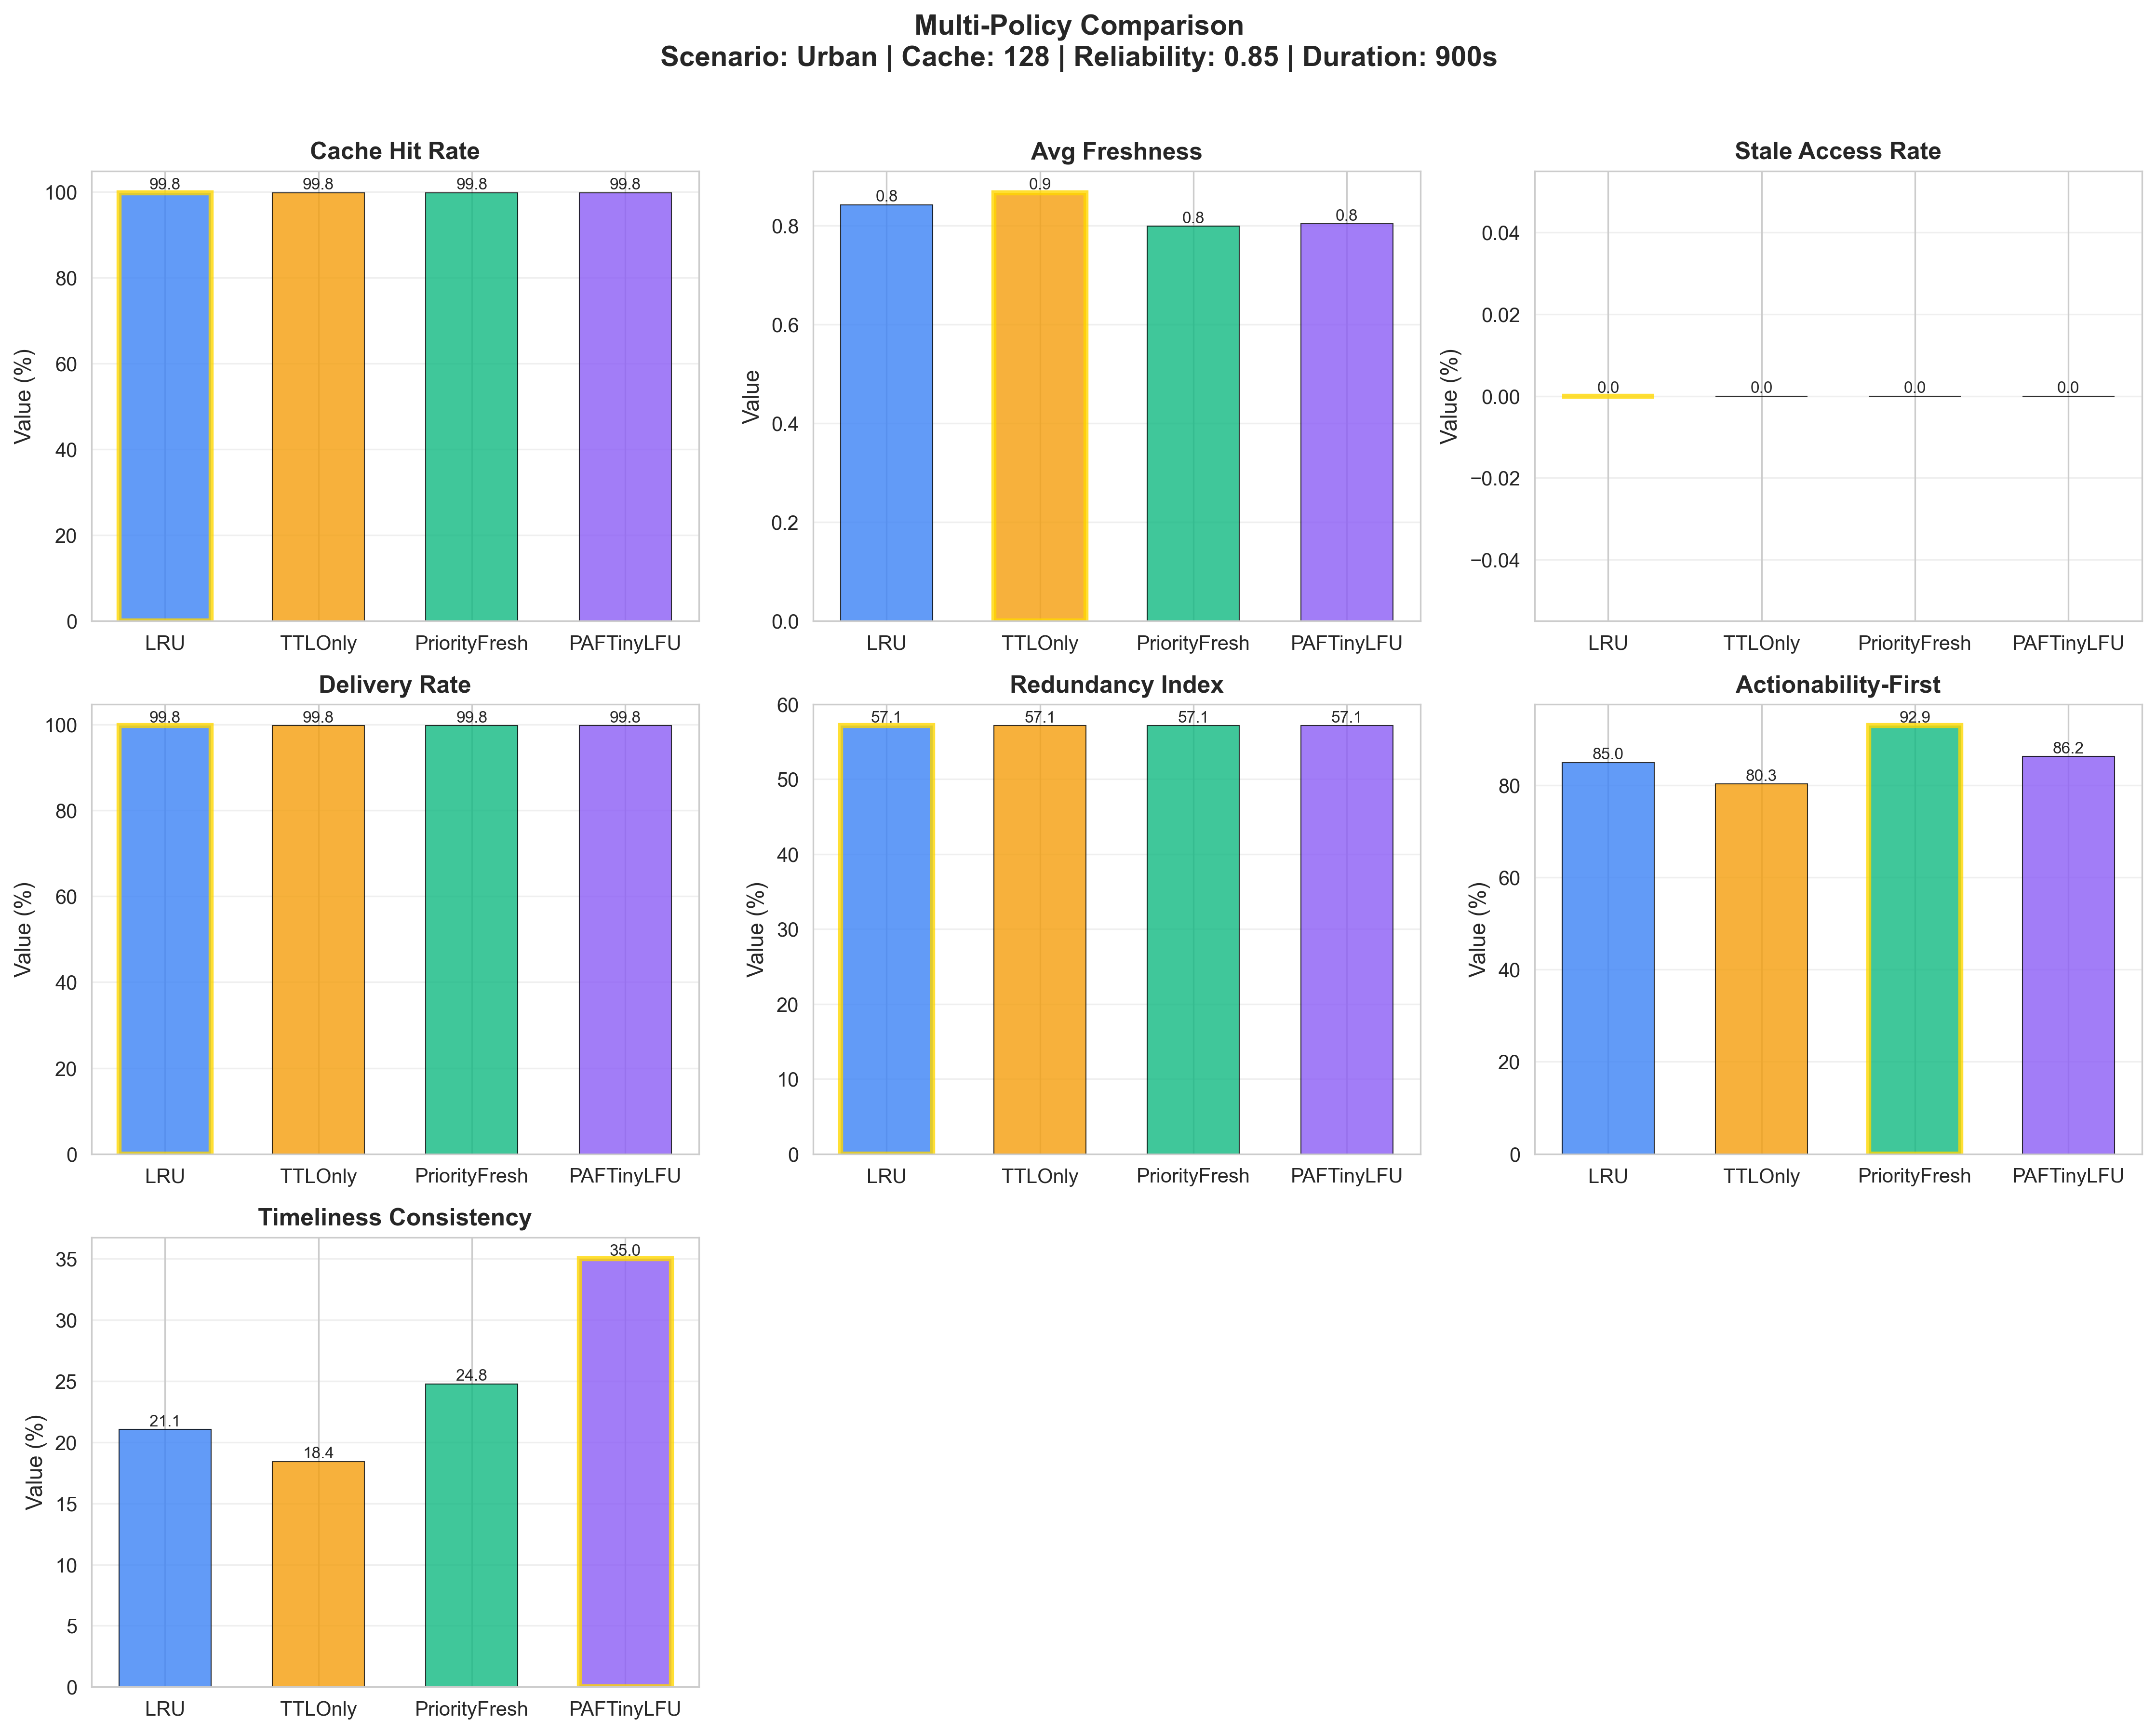
\includegraphics[width=\linewidth]{figures/metrics_grouped_comparison.png}
    \caption{Grouped comparison of key metrics under the baseline configuration for all four policies.}
    \label{fig:baseline-grouped}
\end{figure}

\begin{figure}[h]
    \centering
    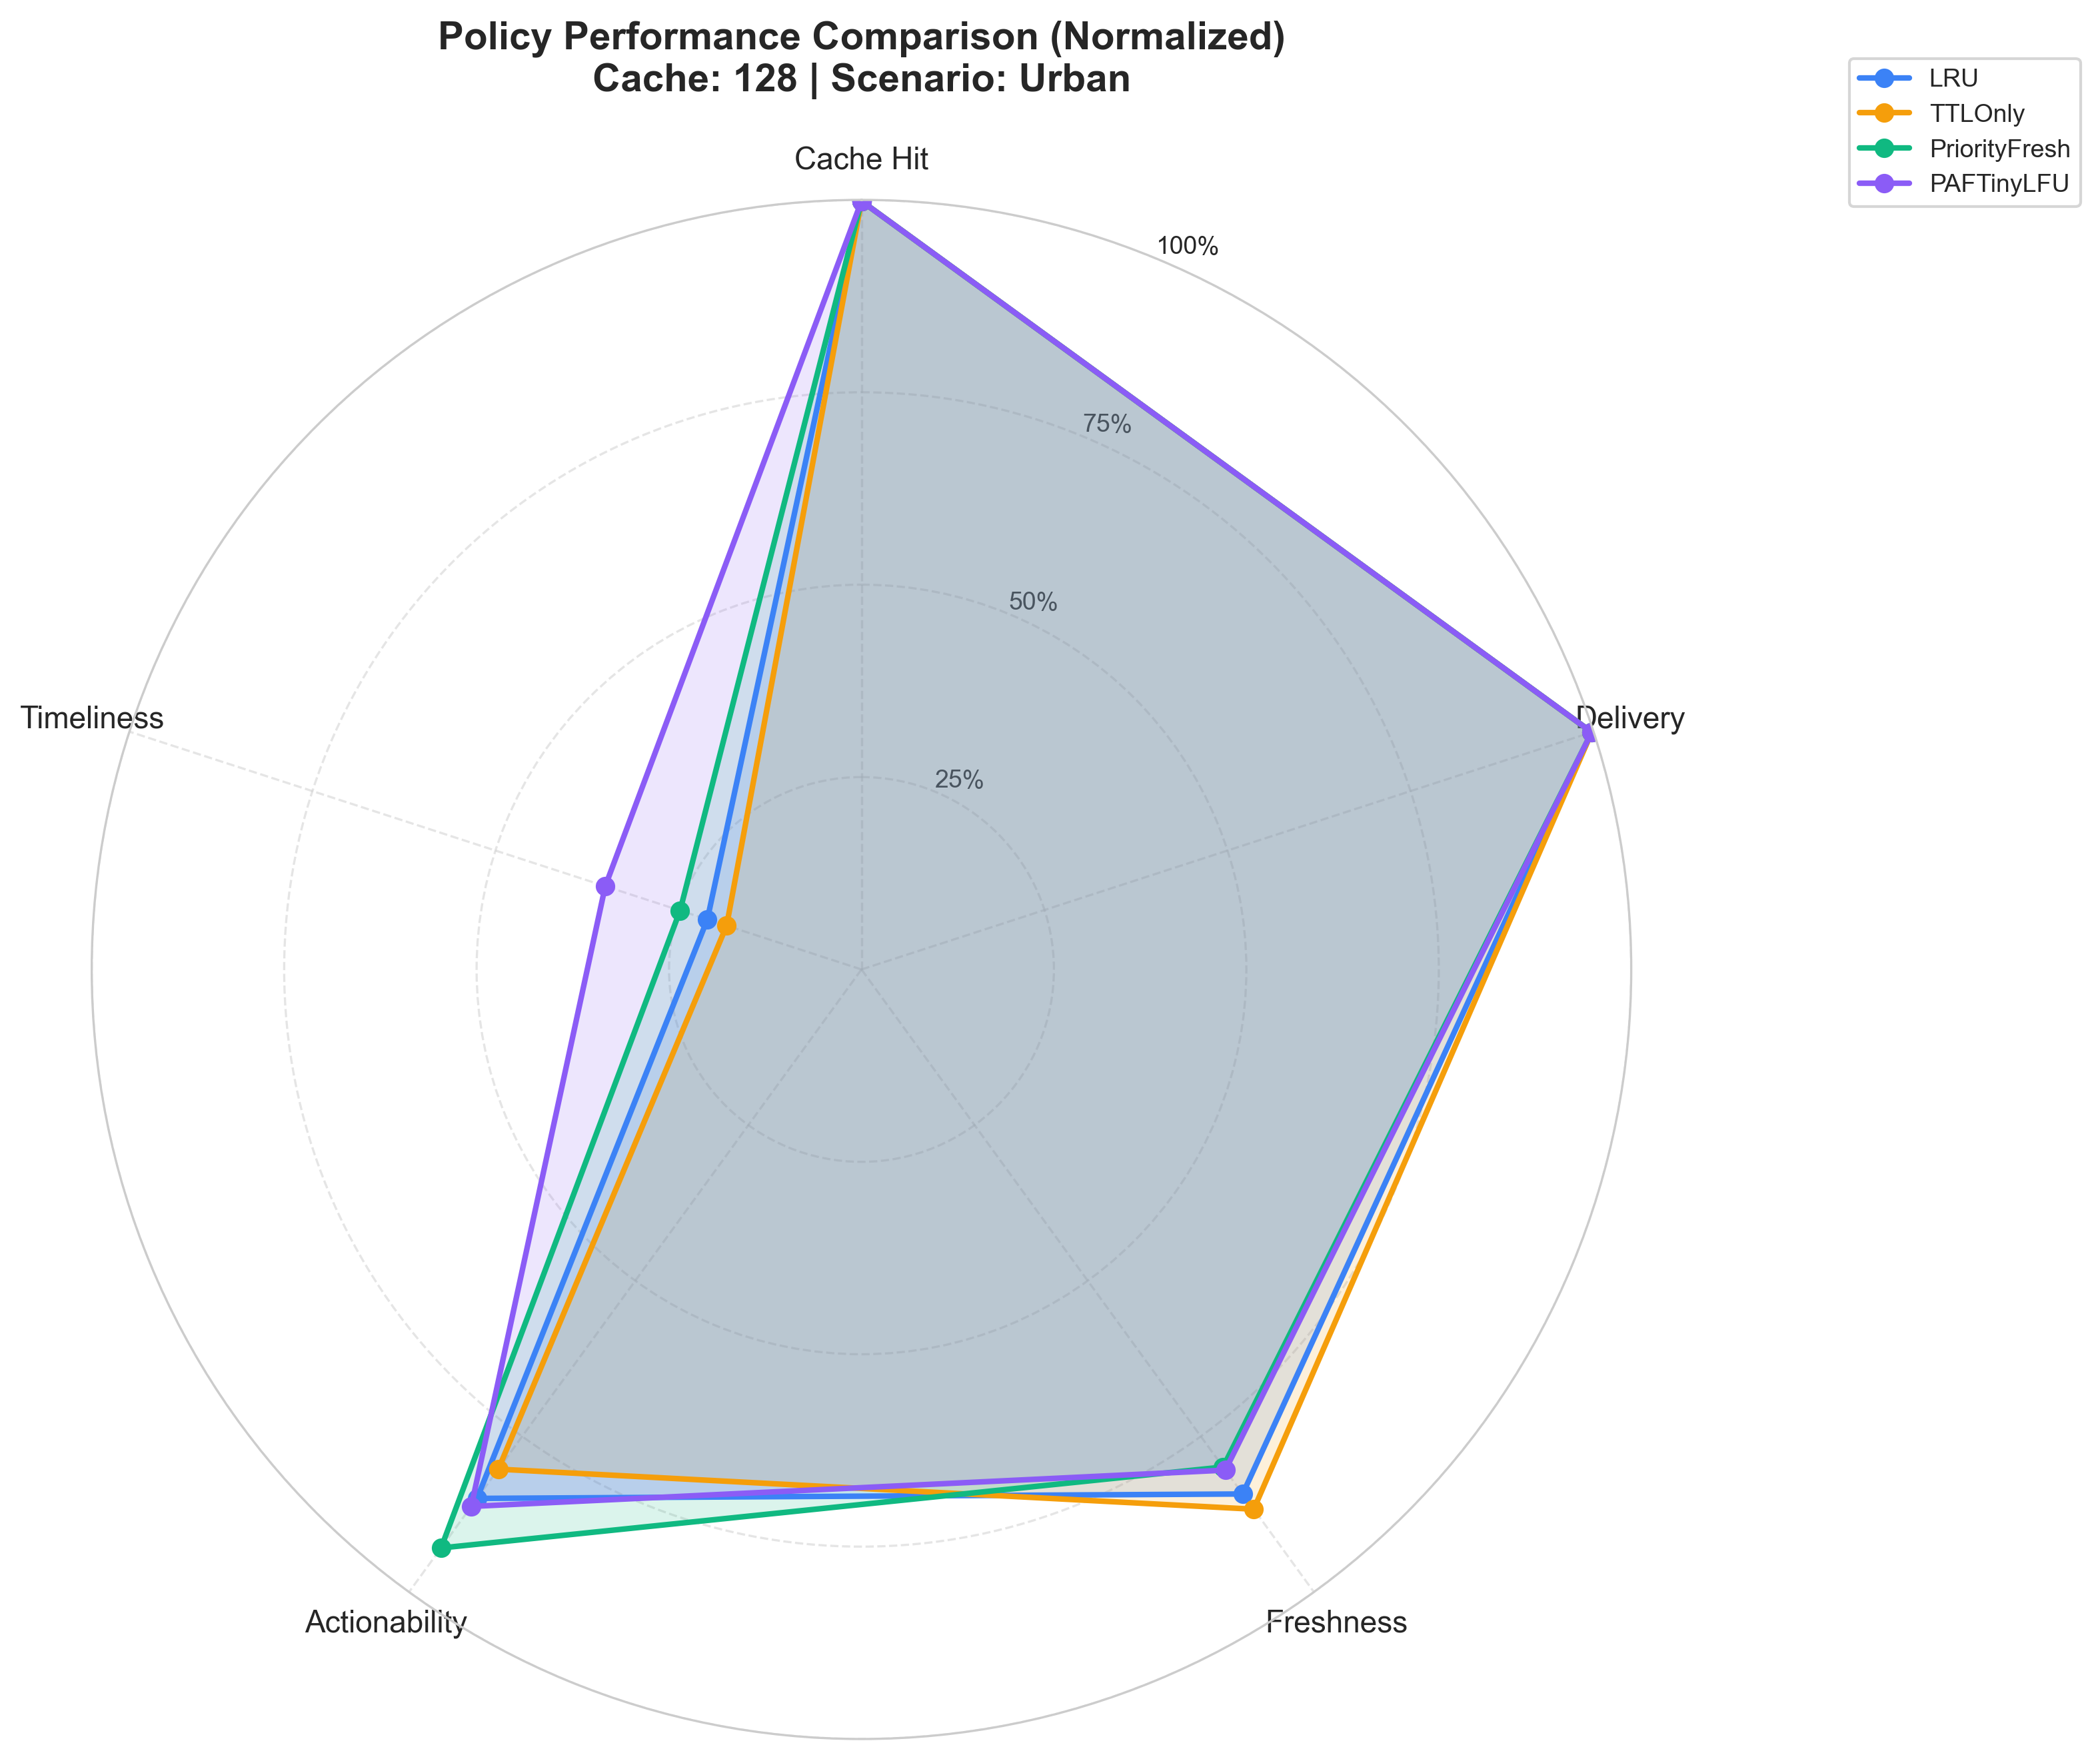
\includegraphics[width=\linewidth]{figures/metrics_radar_comparison.png}
    \caption{Radar plot of normalized metrics under the baseline configuration.}
    \label{fig:baseline-radar}
\end{figure}

\begin{figure}[h]
    \centering
    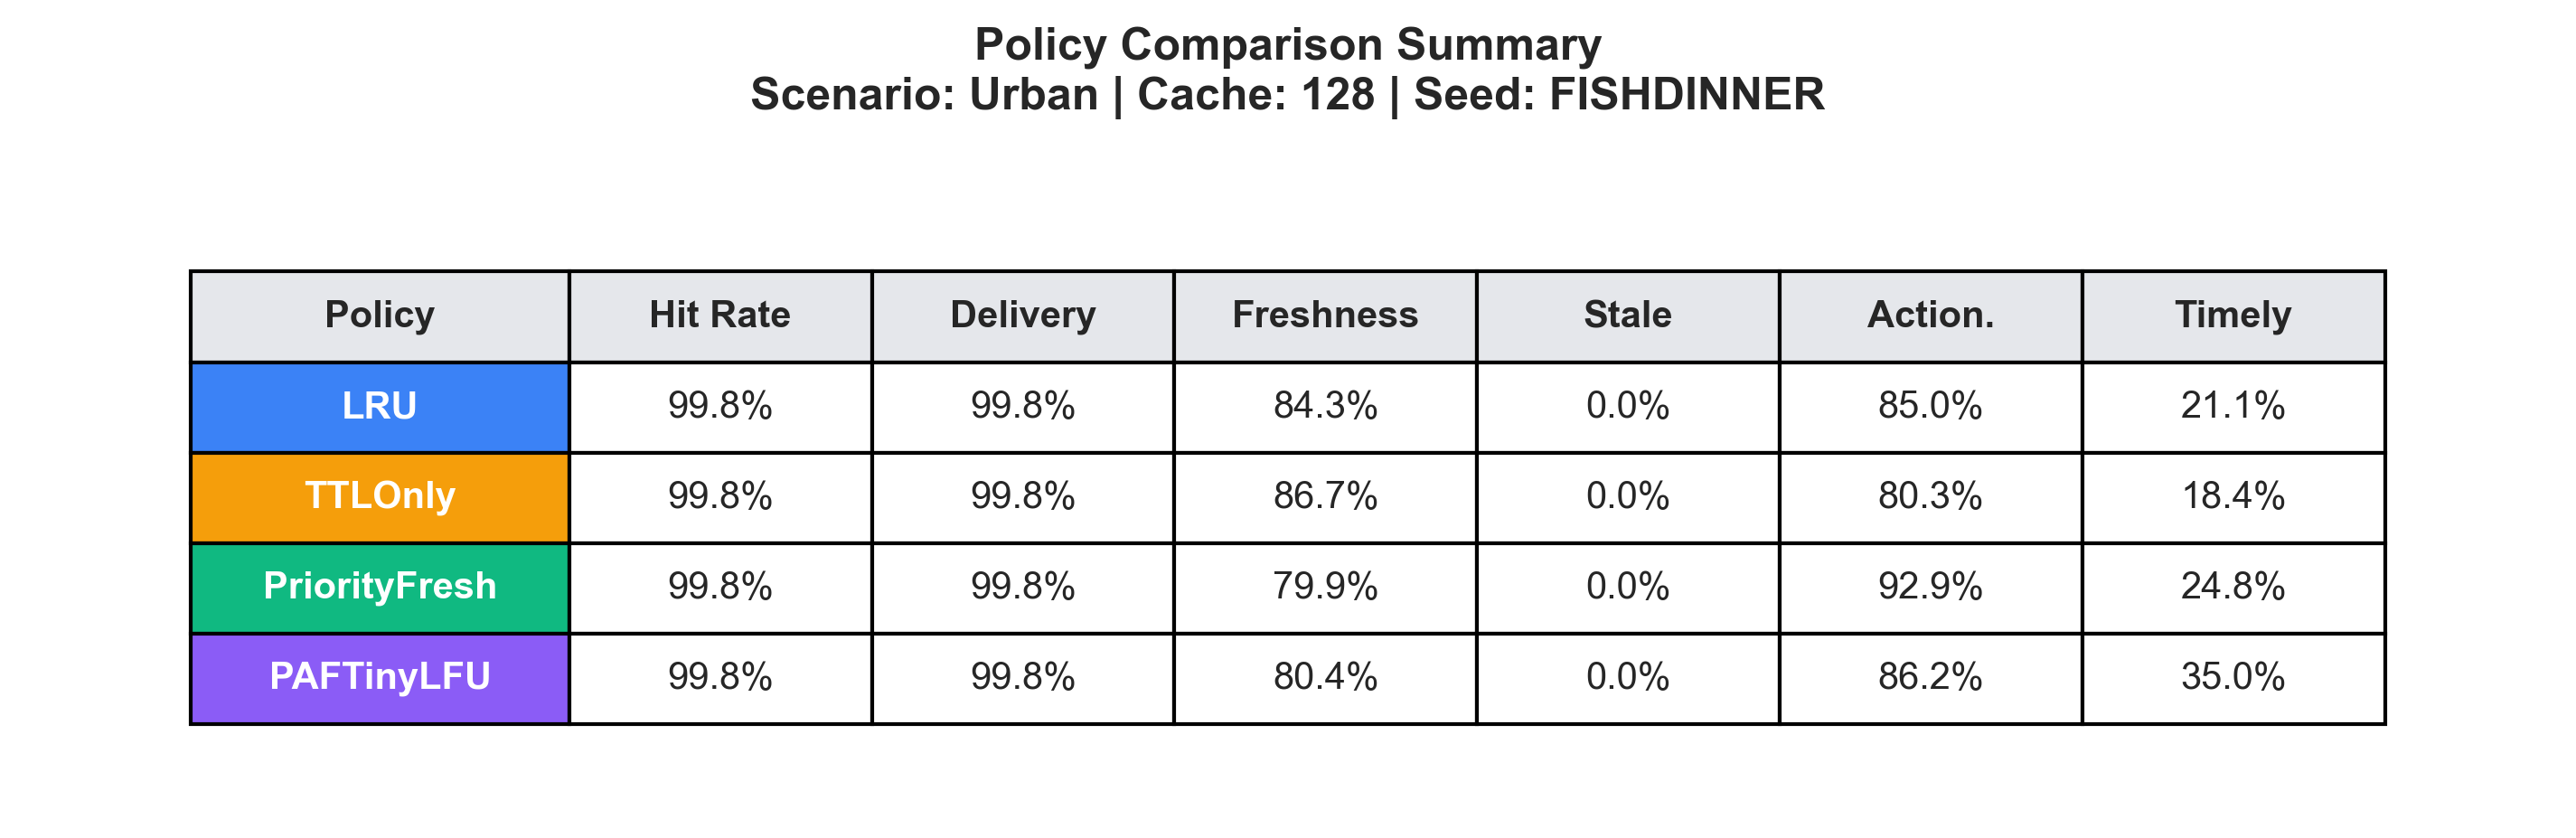
\includegraphics[width=\linewidth]{figures/metrics_summary_table.png}
    \caption{Summary table of baseline metrics across policies.}
    \label{fig:baseline-table}
\end{figure}

\begin{figure}[h]
    \centering
    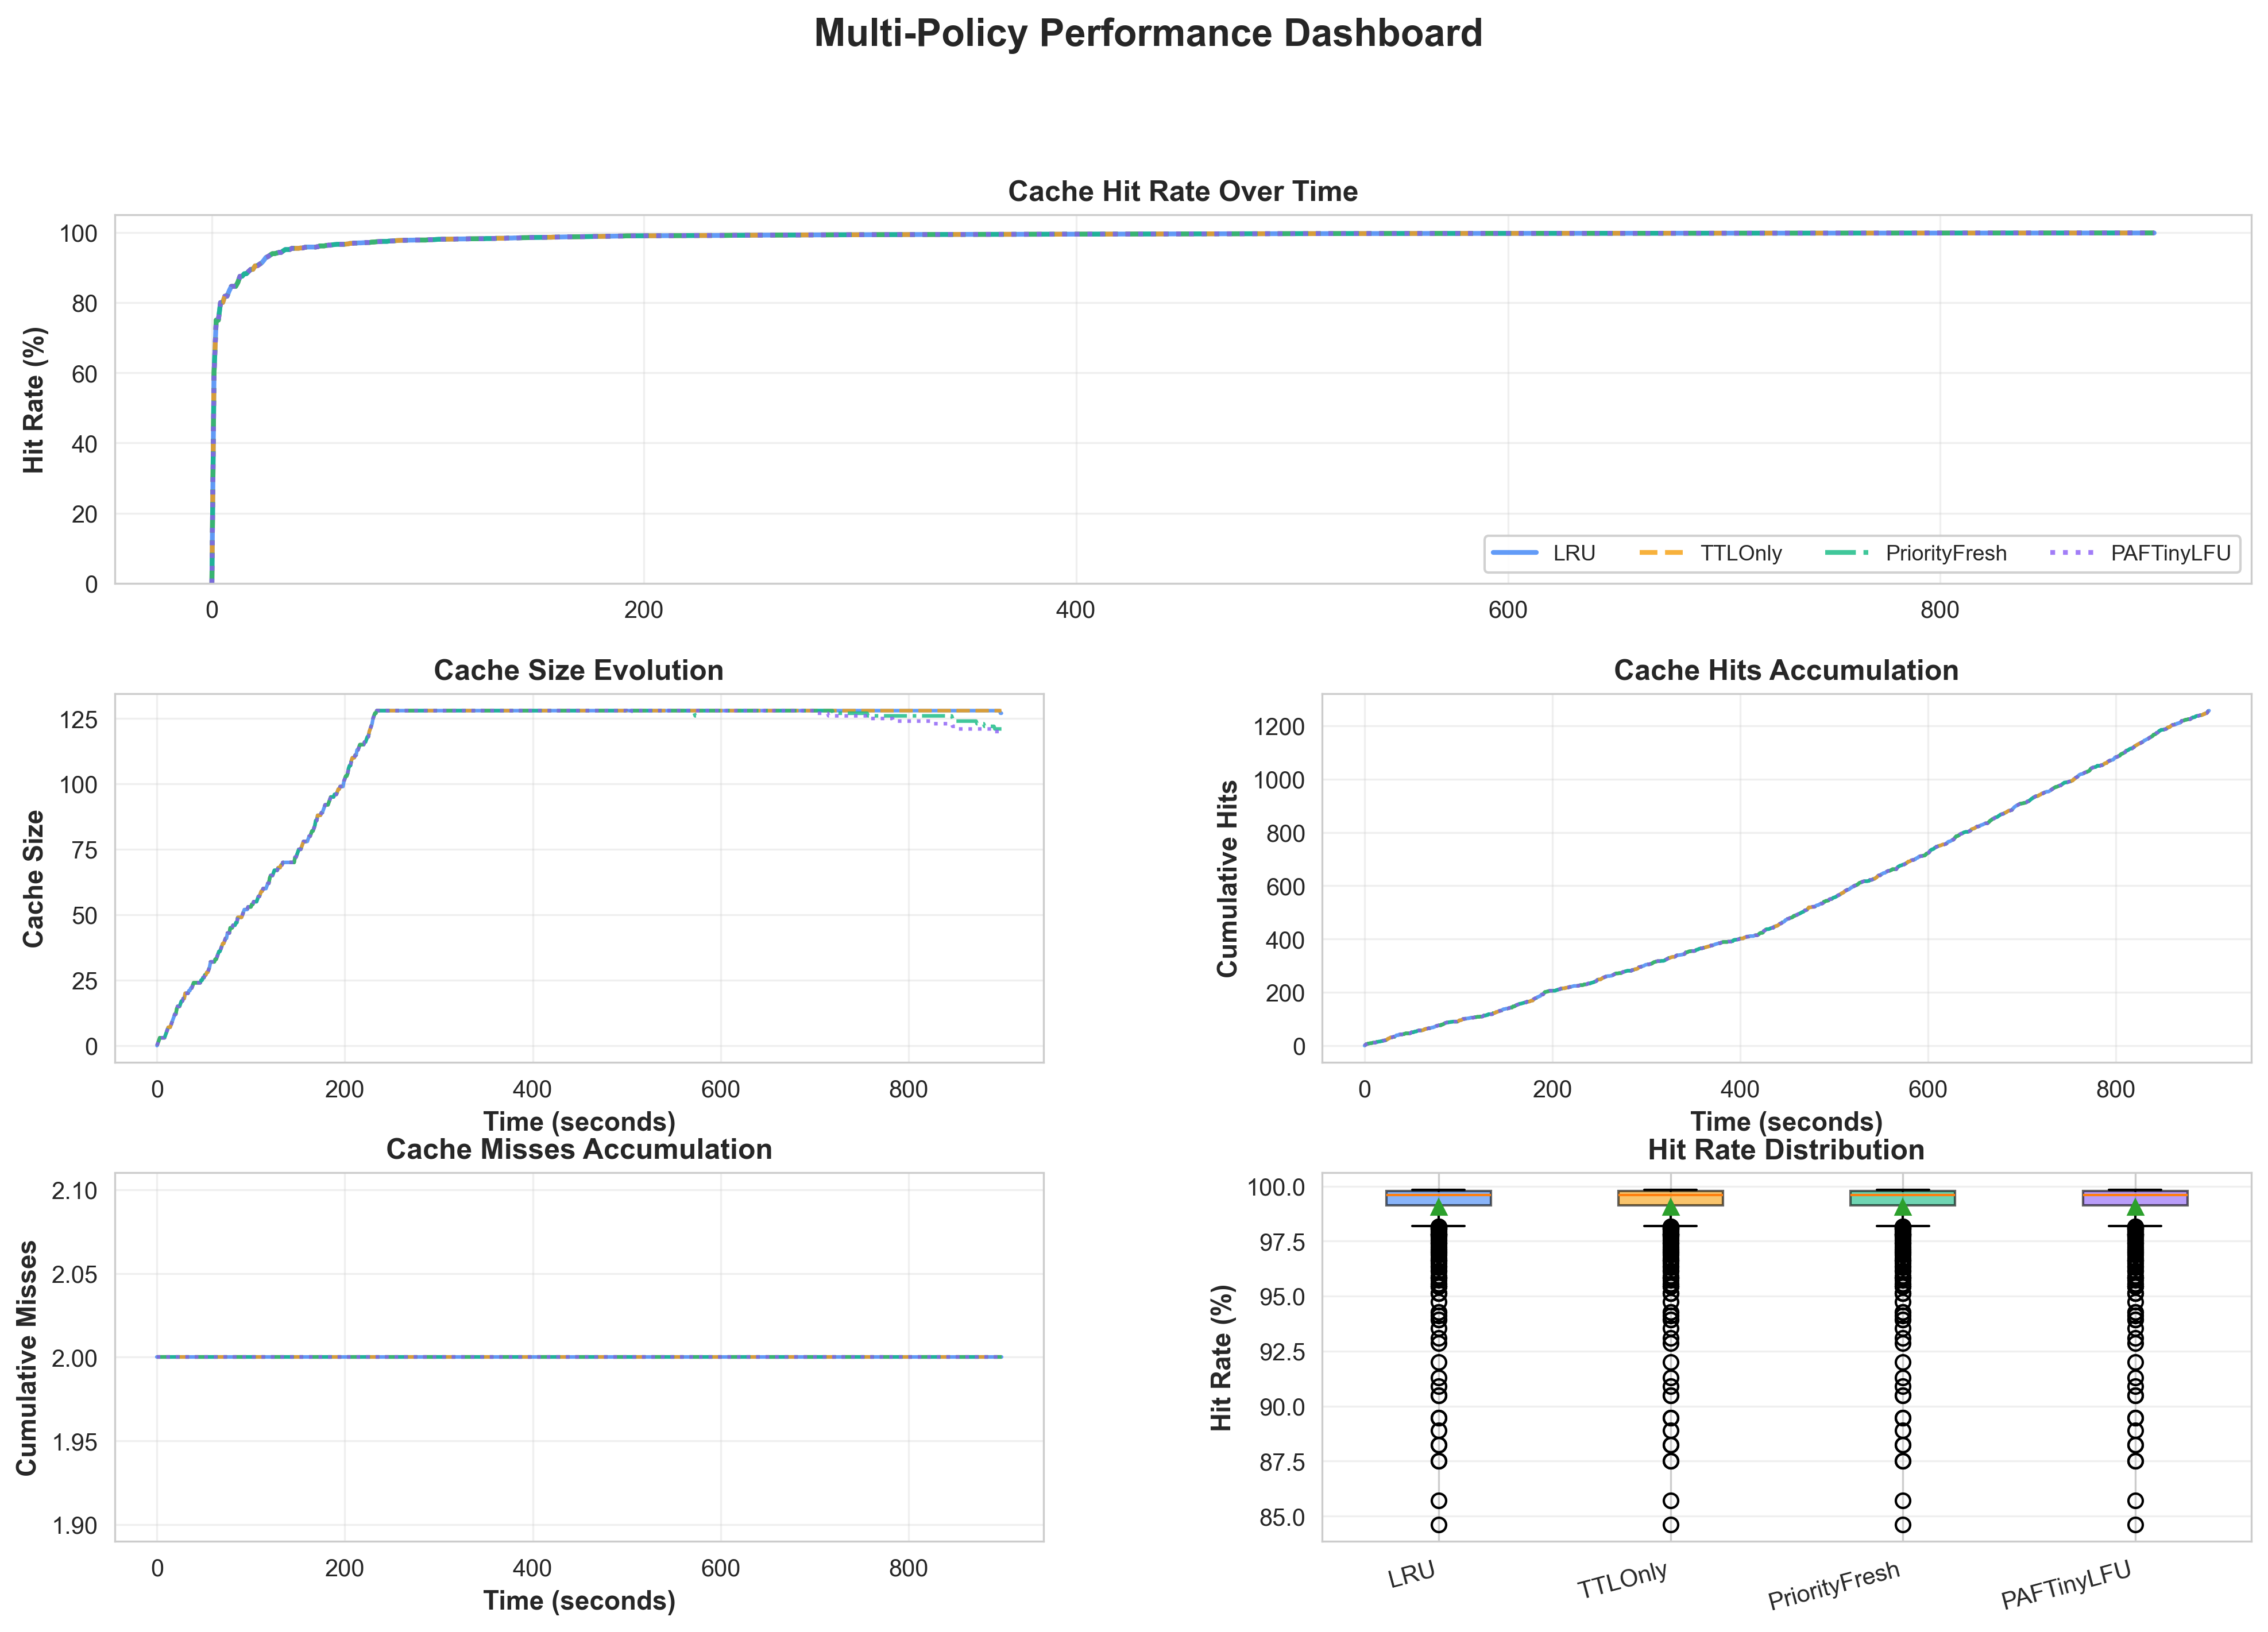
\includegraphics[width=\linewidth]{figures/timeline_dashboard.png}
    \caption{Timeline dashboard view (cache size, hits/misses, and derived hit rate over run time).}
    \label{fig:timeline-dashboard}
\end{figure}

\subsubsection{Cache-size sweep}
\begin{figure}[h]
    \centering
    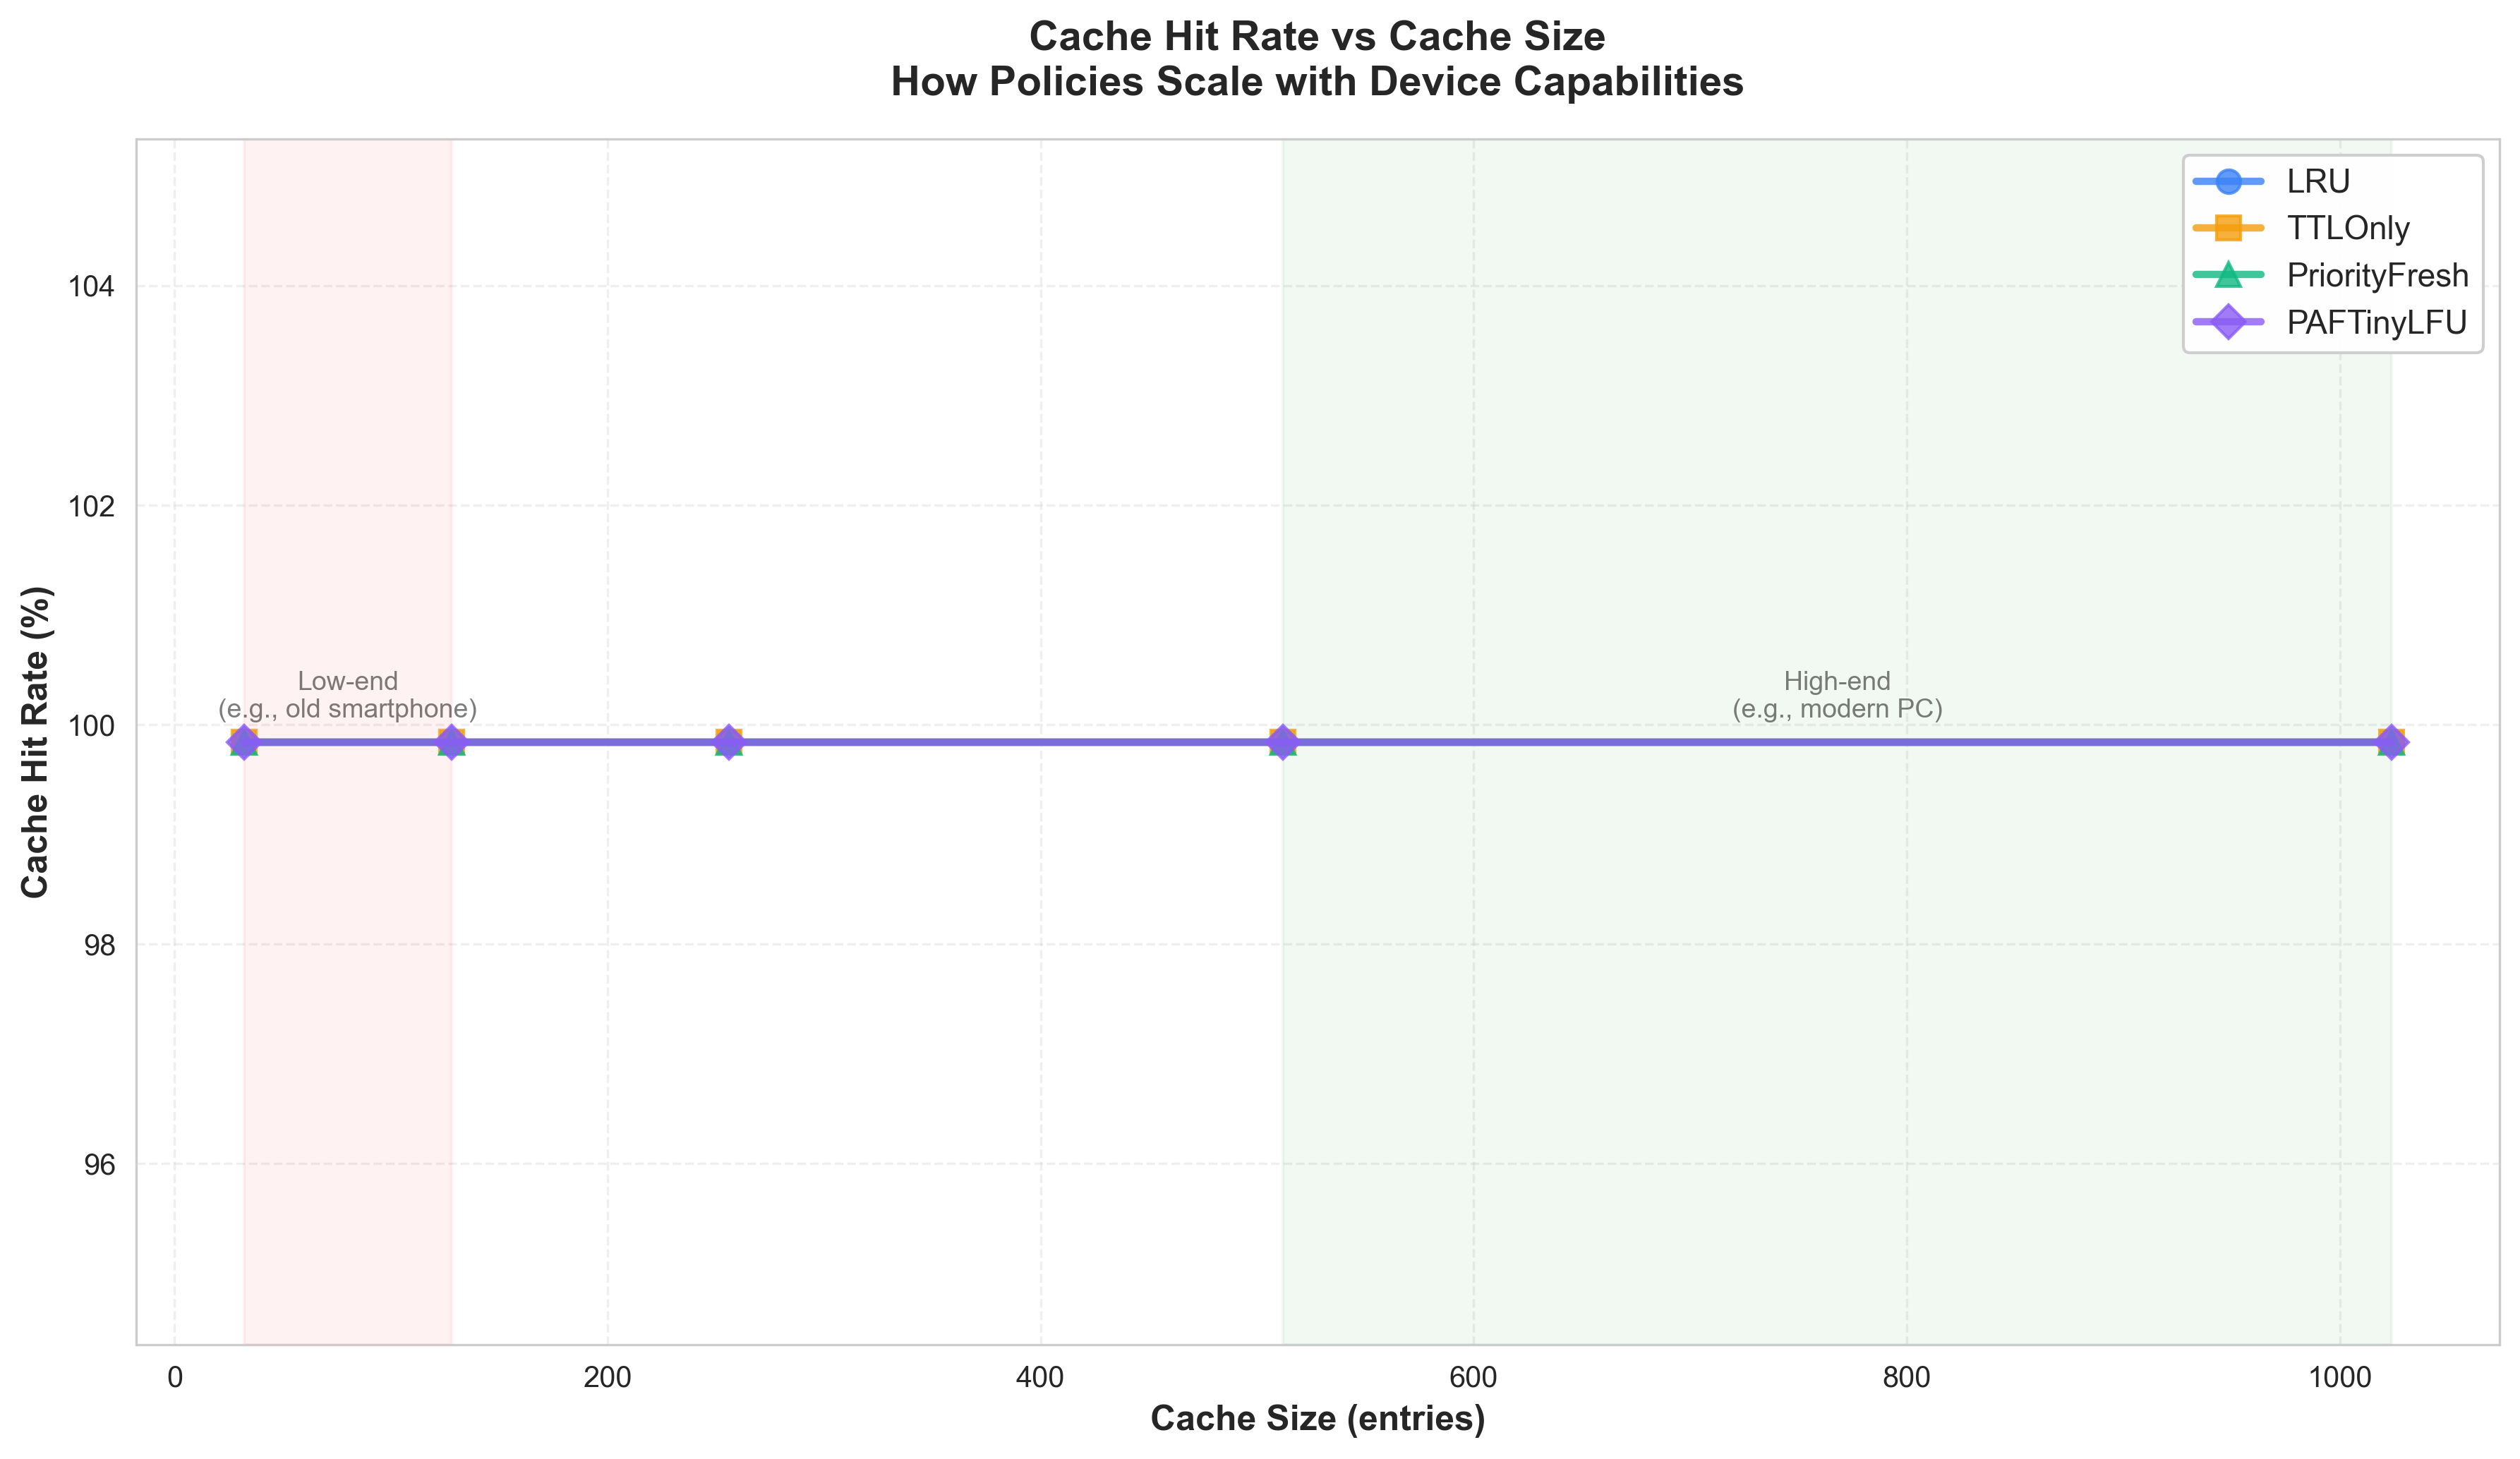
\includegraphics[width=\linewidth]{figures/device_scaling_cacheHitRate.png}
    \caption{Cache-size scaling: cache hit rate across policies.}
    \label{fig:device-scaling-cachehit}
\end{figure}

\begin{figure}[h]
    \centering
    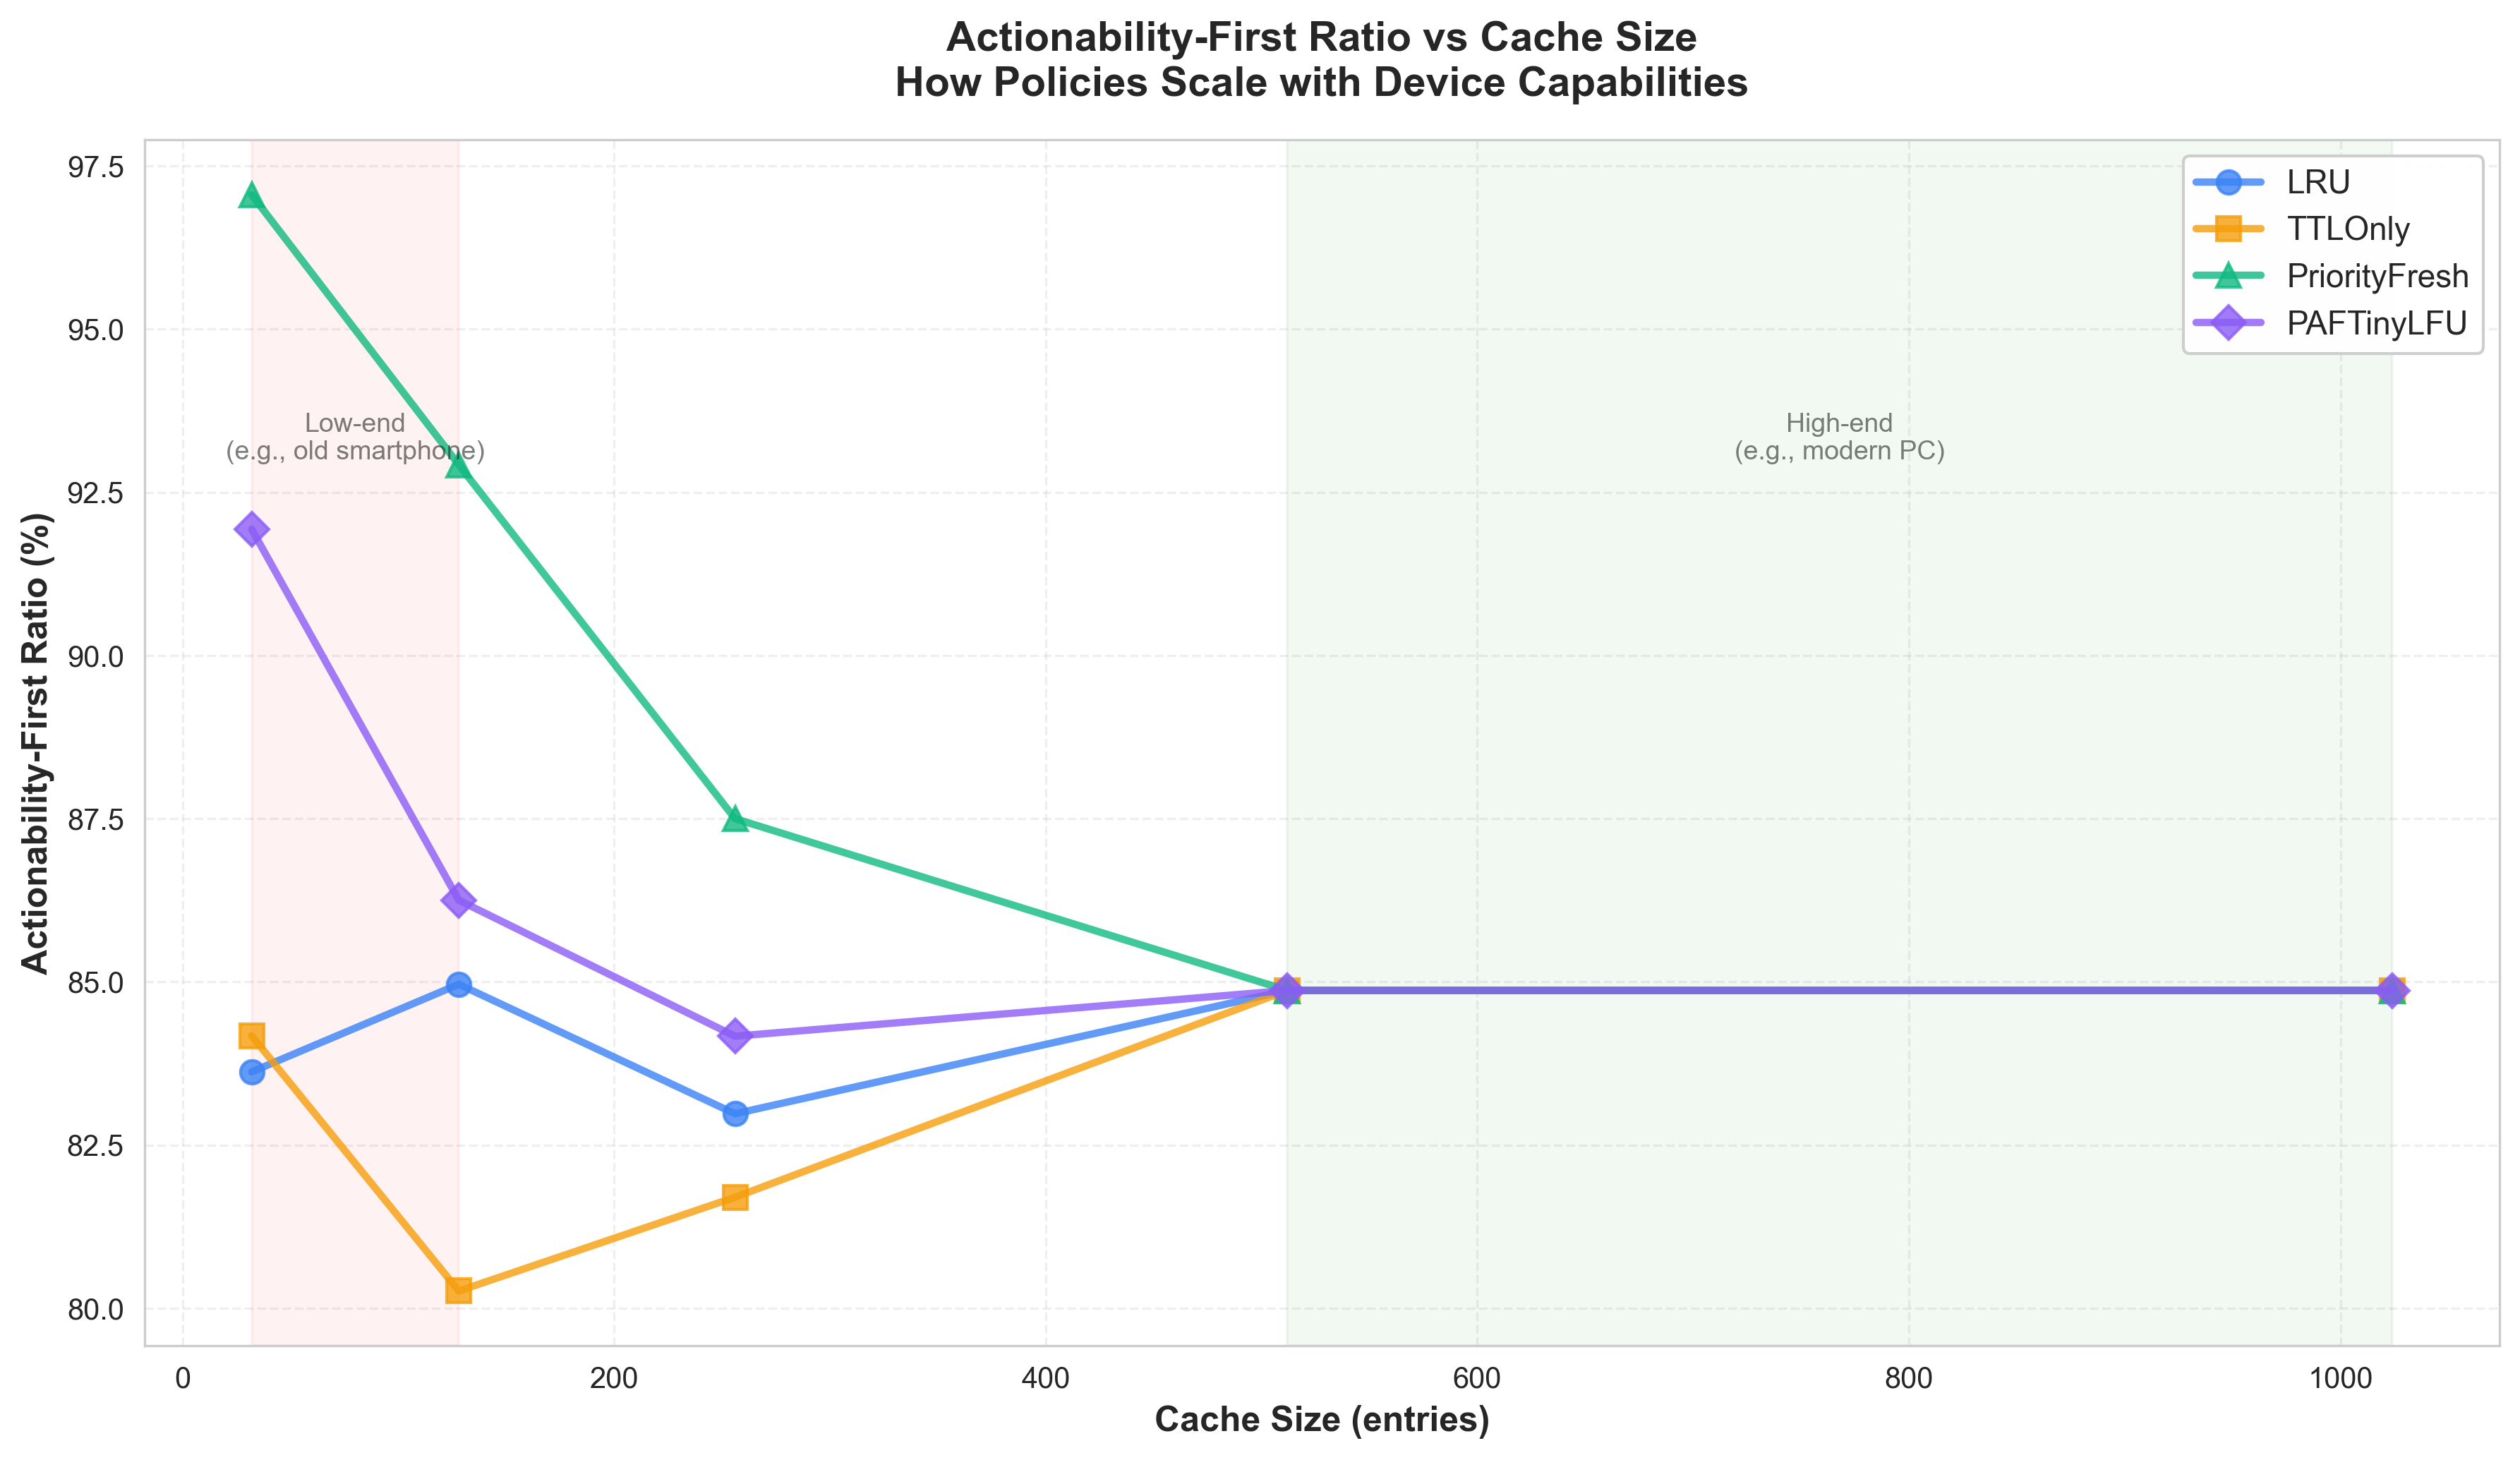
\includegraphics[width=\linewidth]{figures/device_scaling_actionabilityFirstRatio.png}
    \caption{Cache-size scaling: actionability-first ratio across policies.}
    \label{fig:device-scaling-actionability}
\end{figure}

\begin{figure}[h]
    \centering
    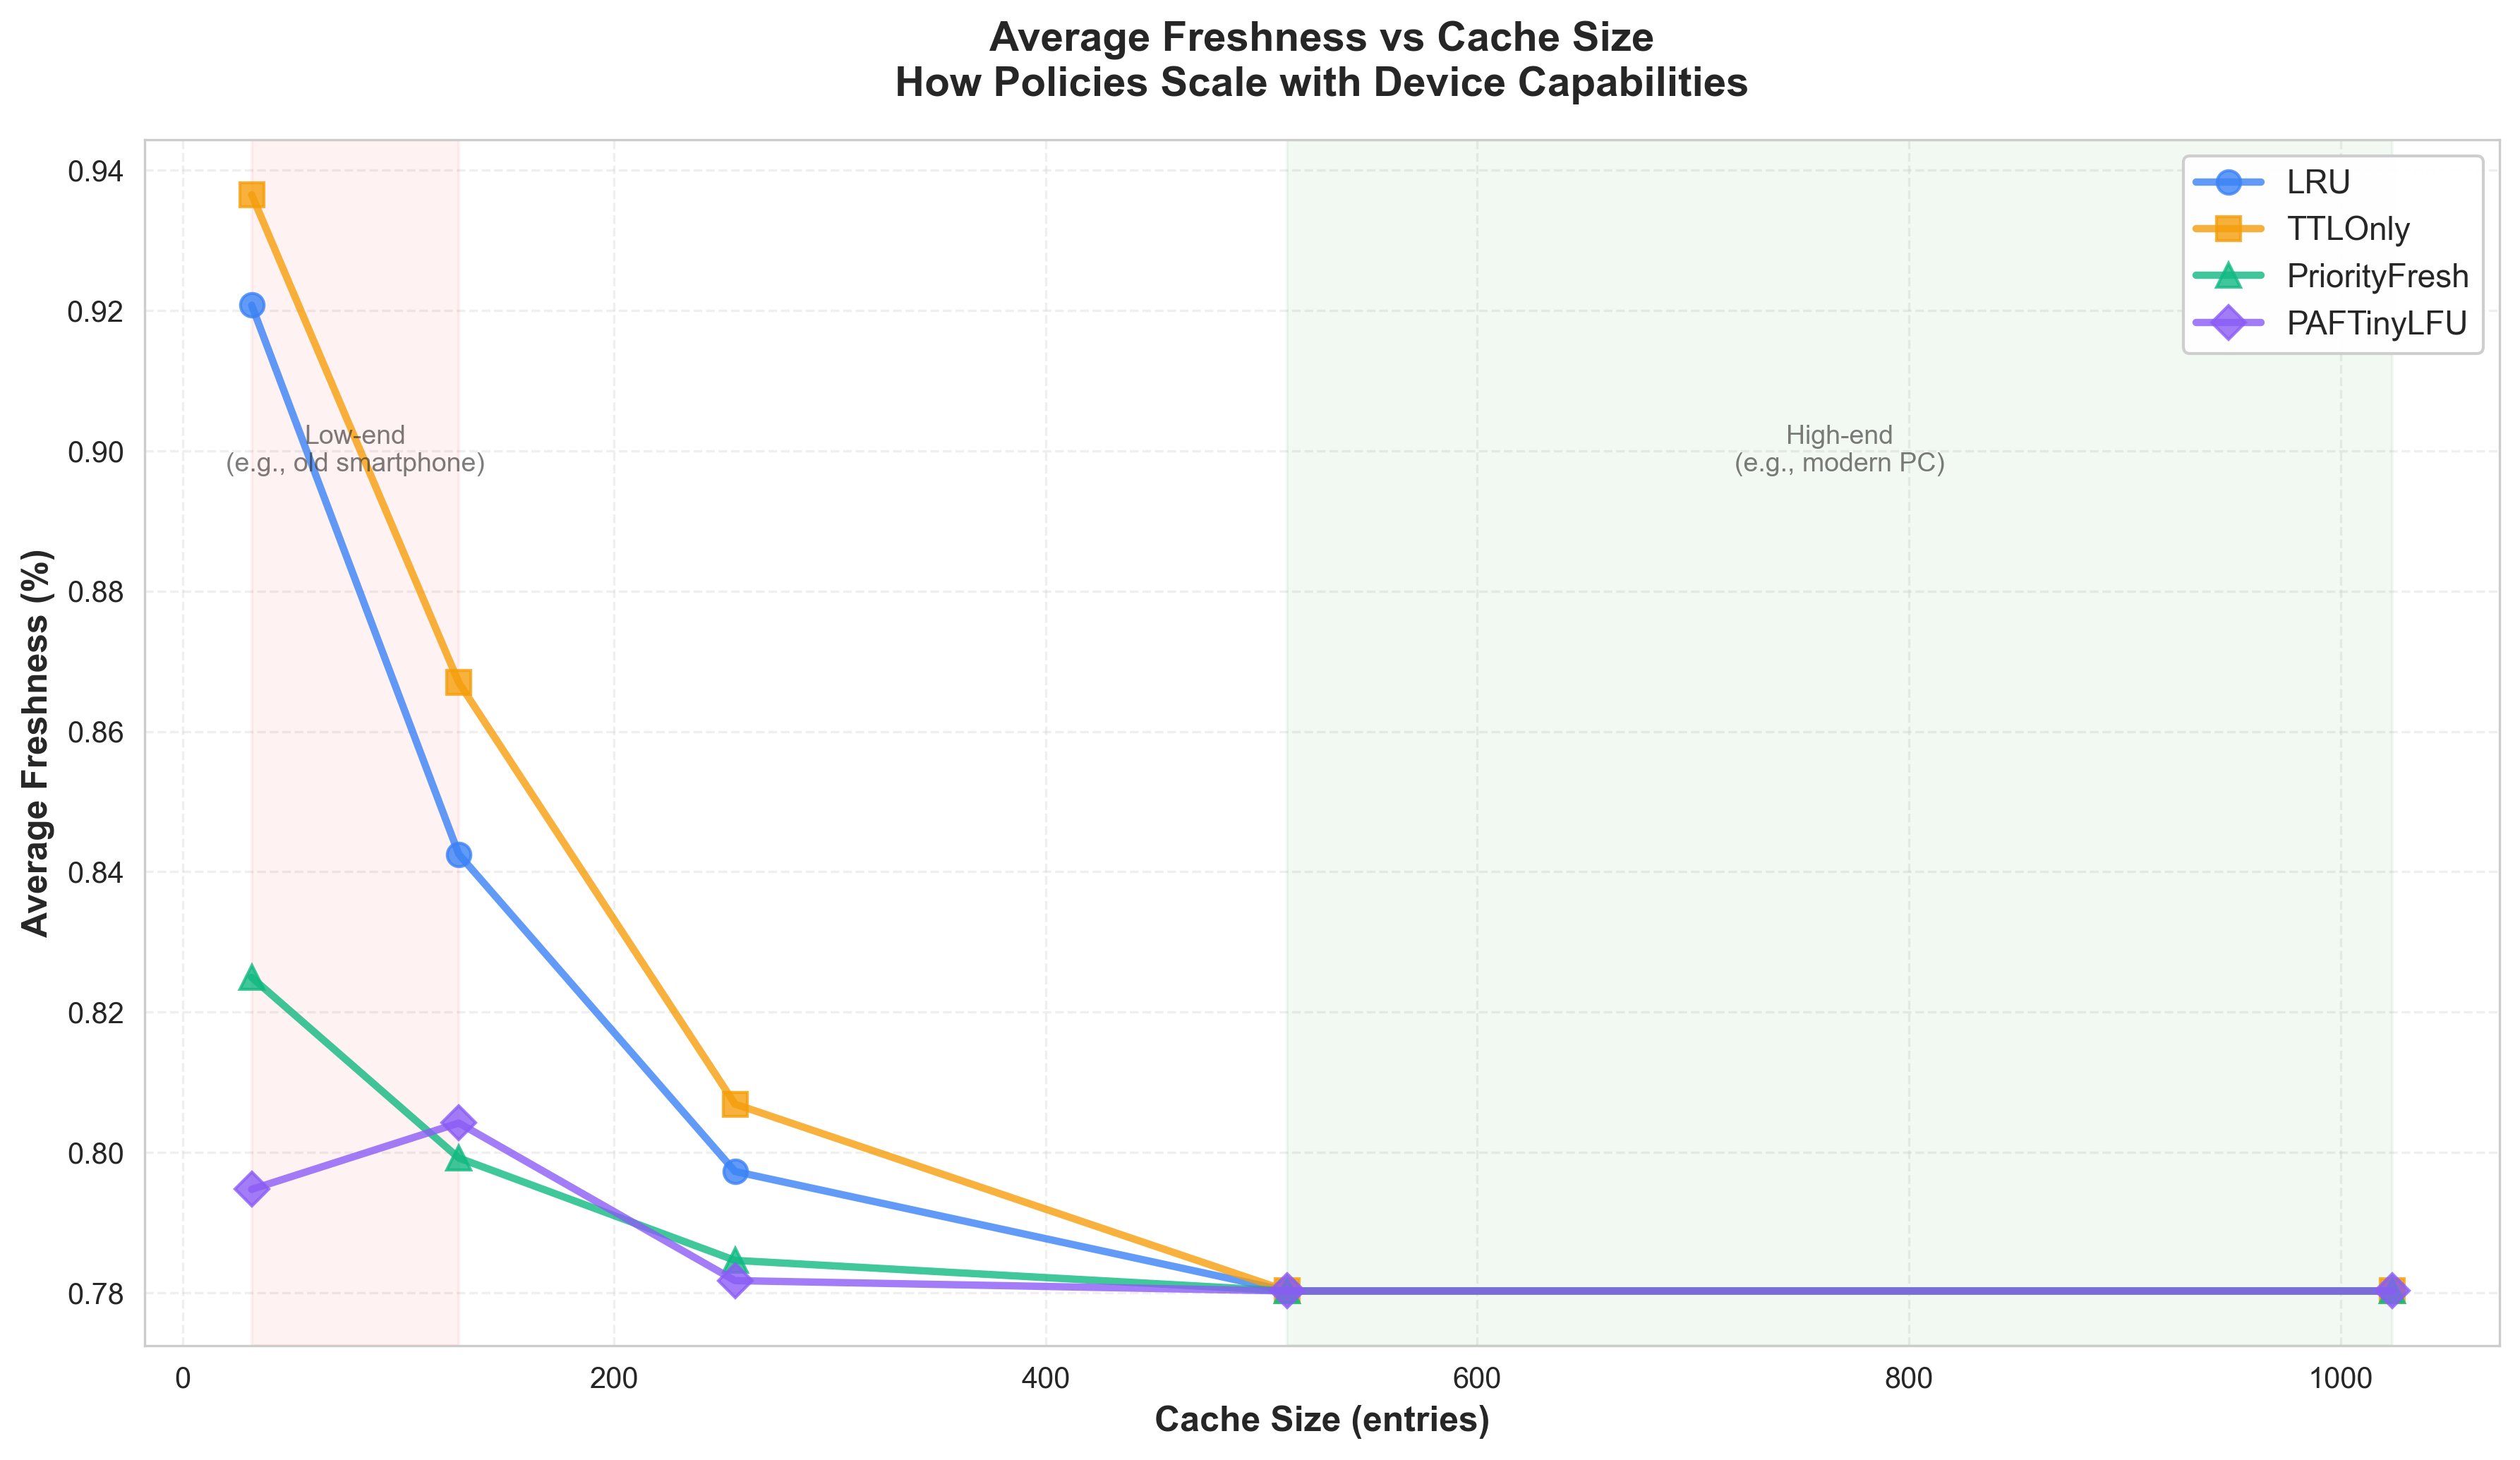
\includegraphics[width=\linewidth]{figures/device_scaling_avgFreshness.png}
    \caption{Cache-size scaling: average freshness across policies.}
    \label{fig:device-scaling-freshness}
\end{figure}

\begin{figure}[h]
    \centering
    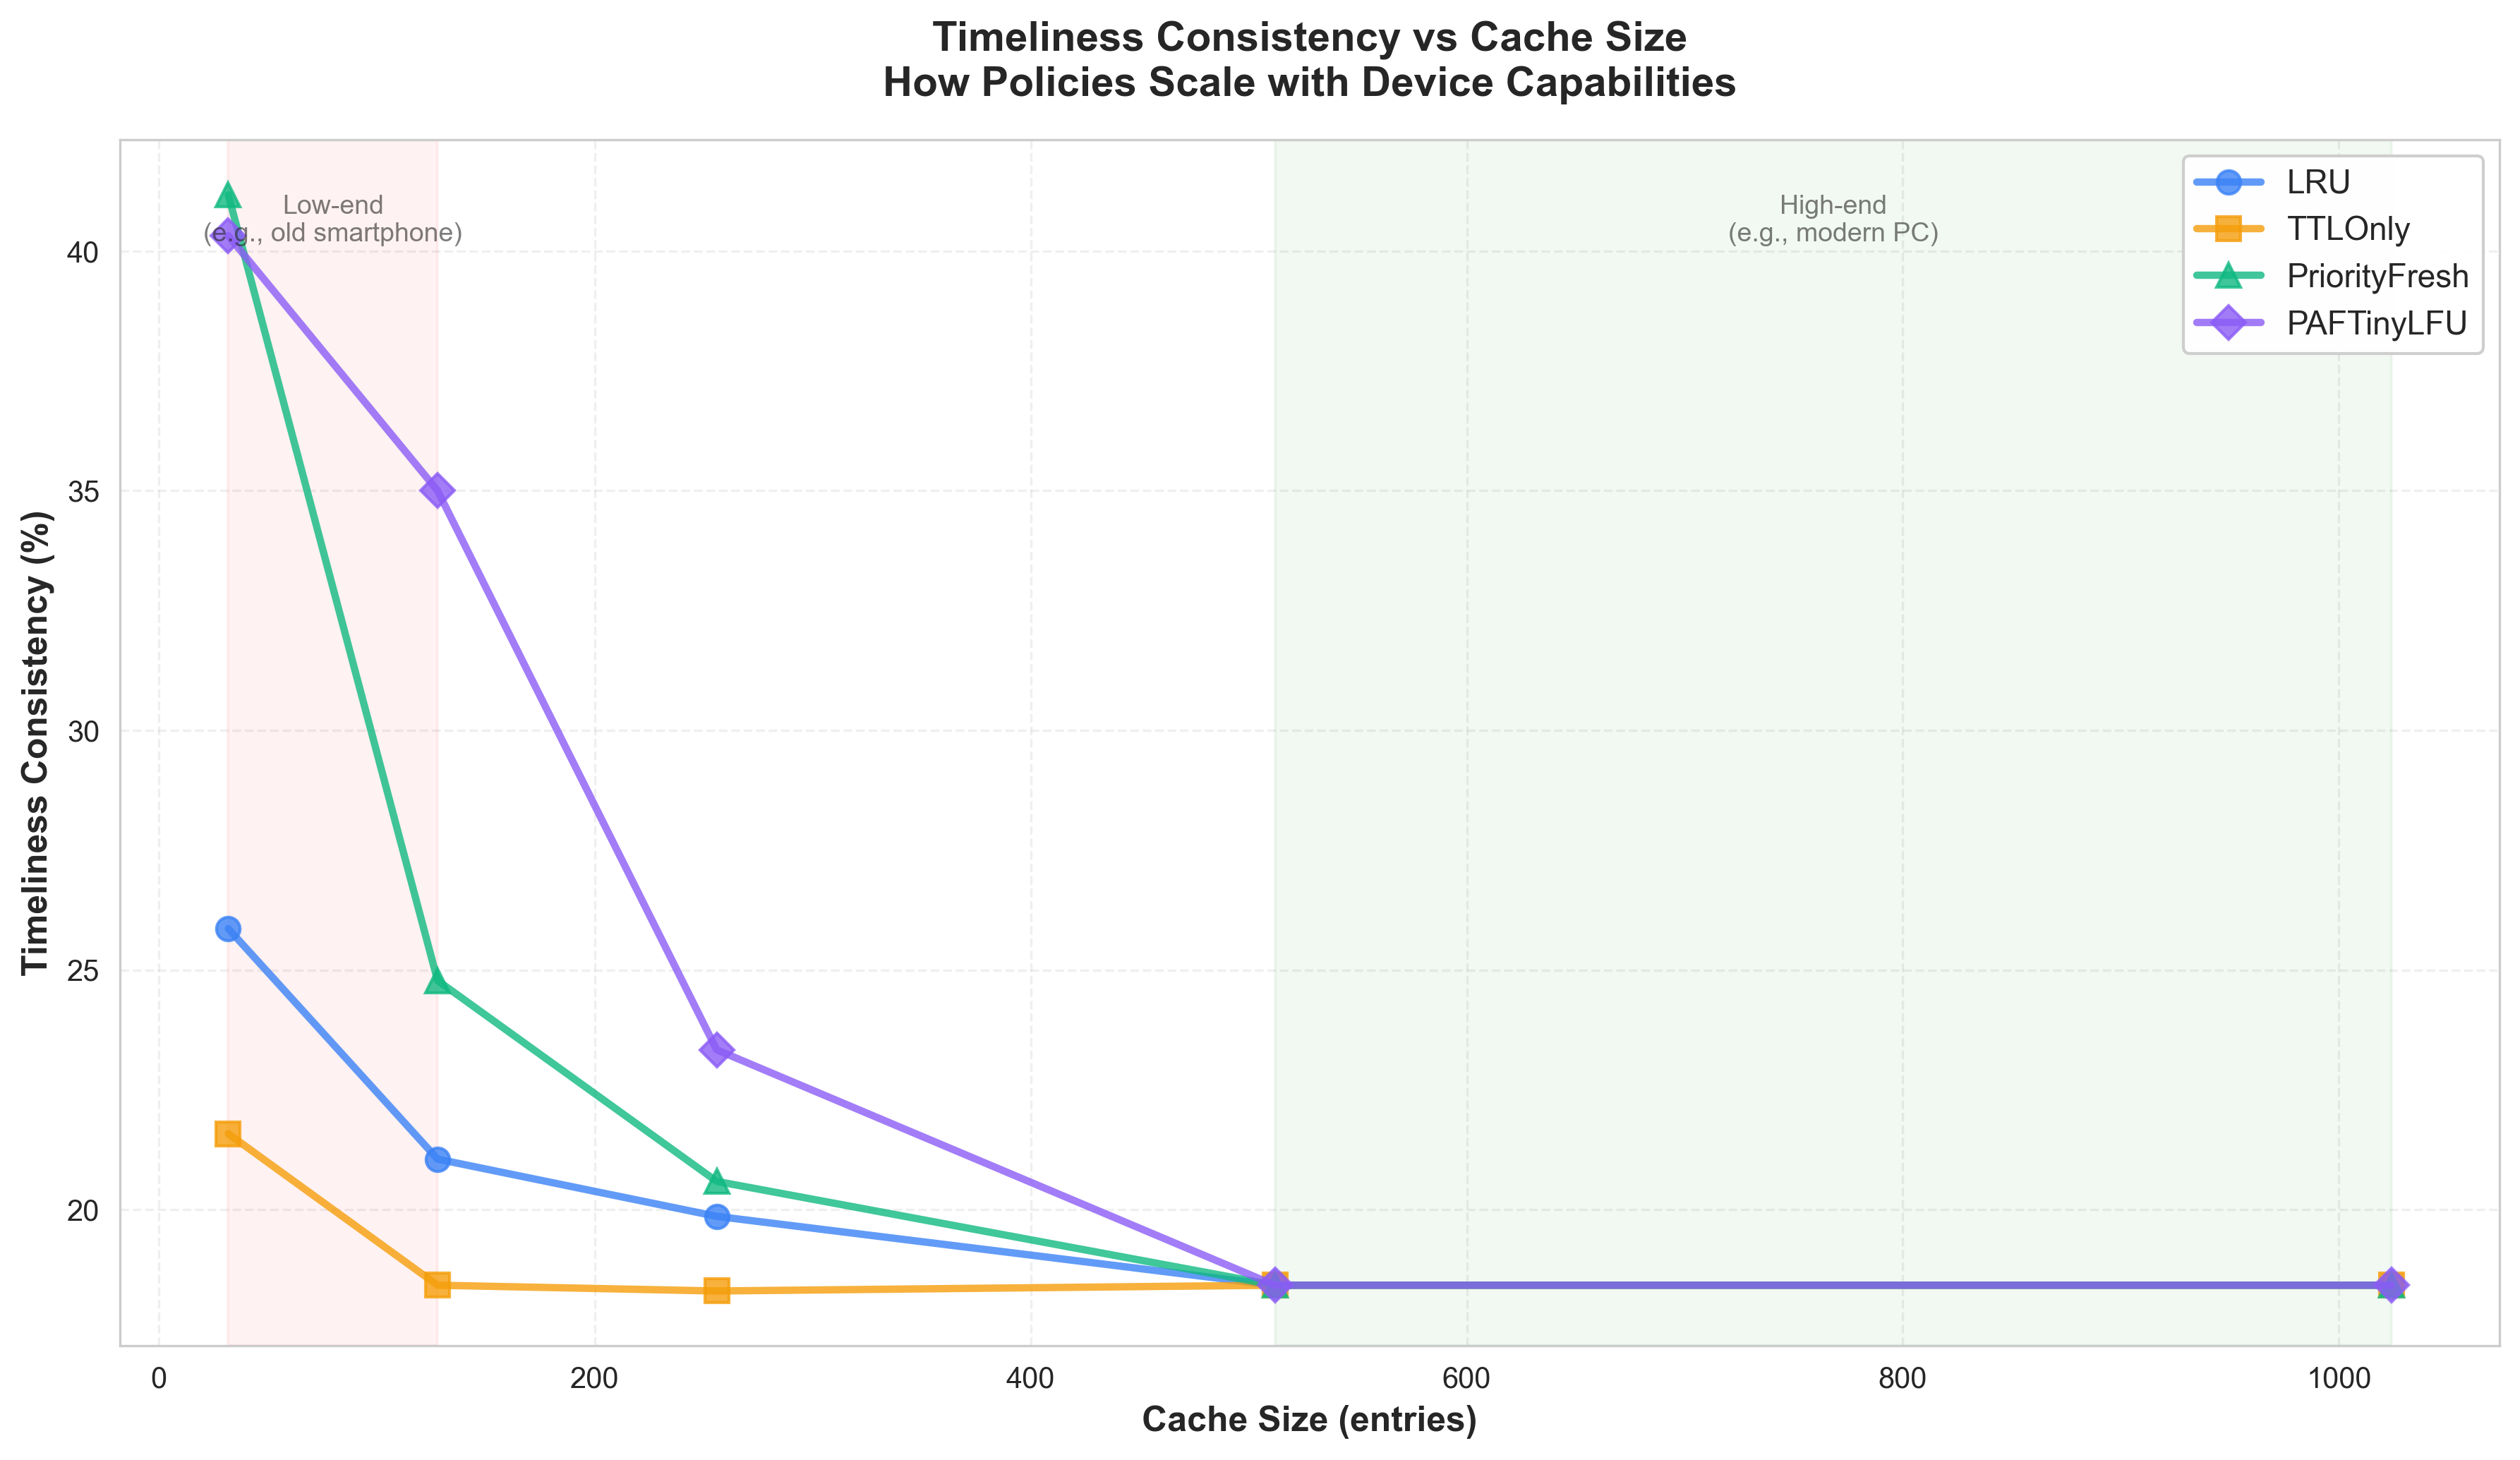
\includegraphics[width=\linewidth]{figures/device_scaling_timelinessConsistency.png}
    \caption{Cache-size scaling: timeliness consistency across policies.}
    \label{fig:device-scaling-timeliness}
\end{figure}

\begin{figure}[h]
    \centering
    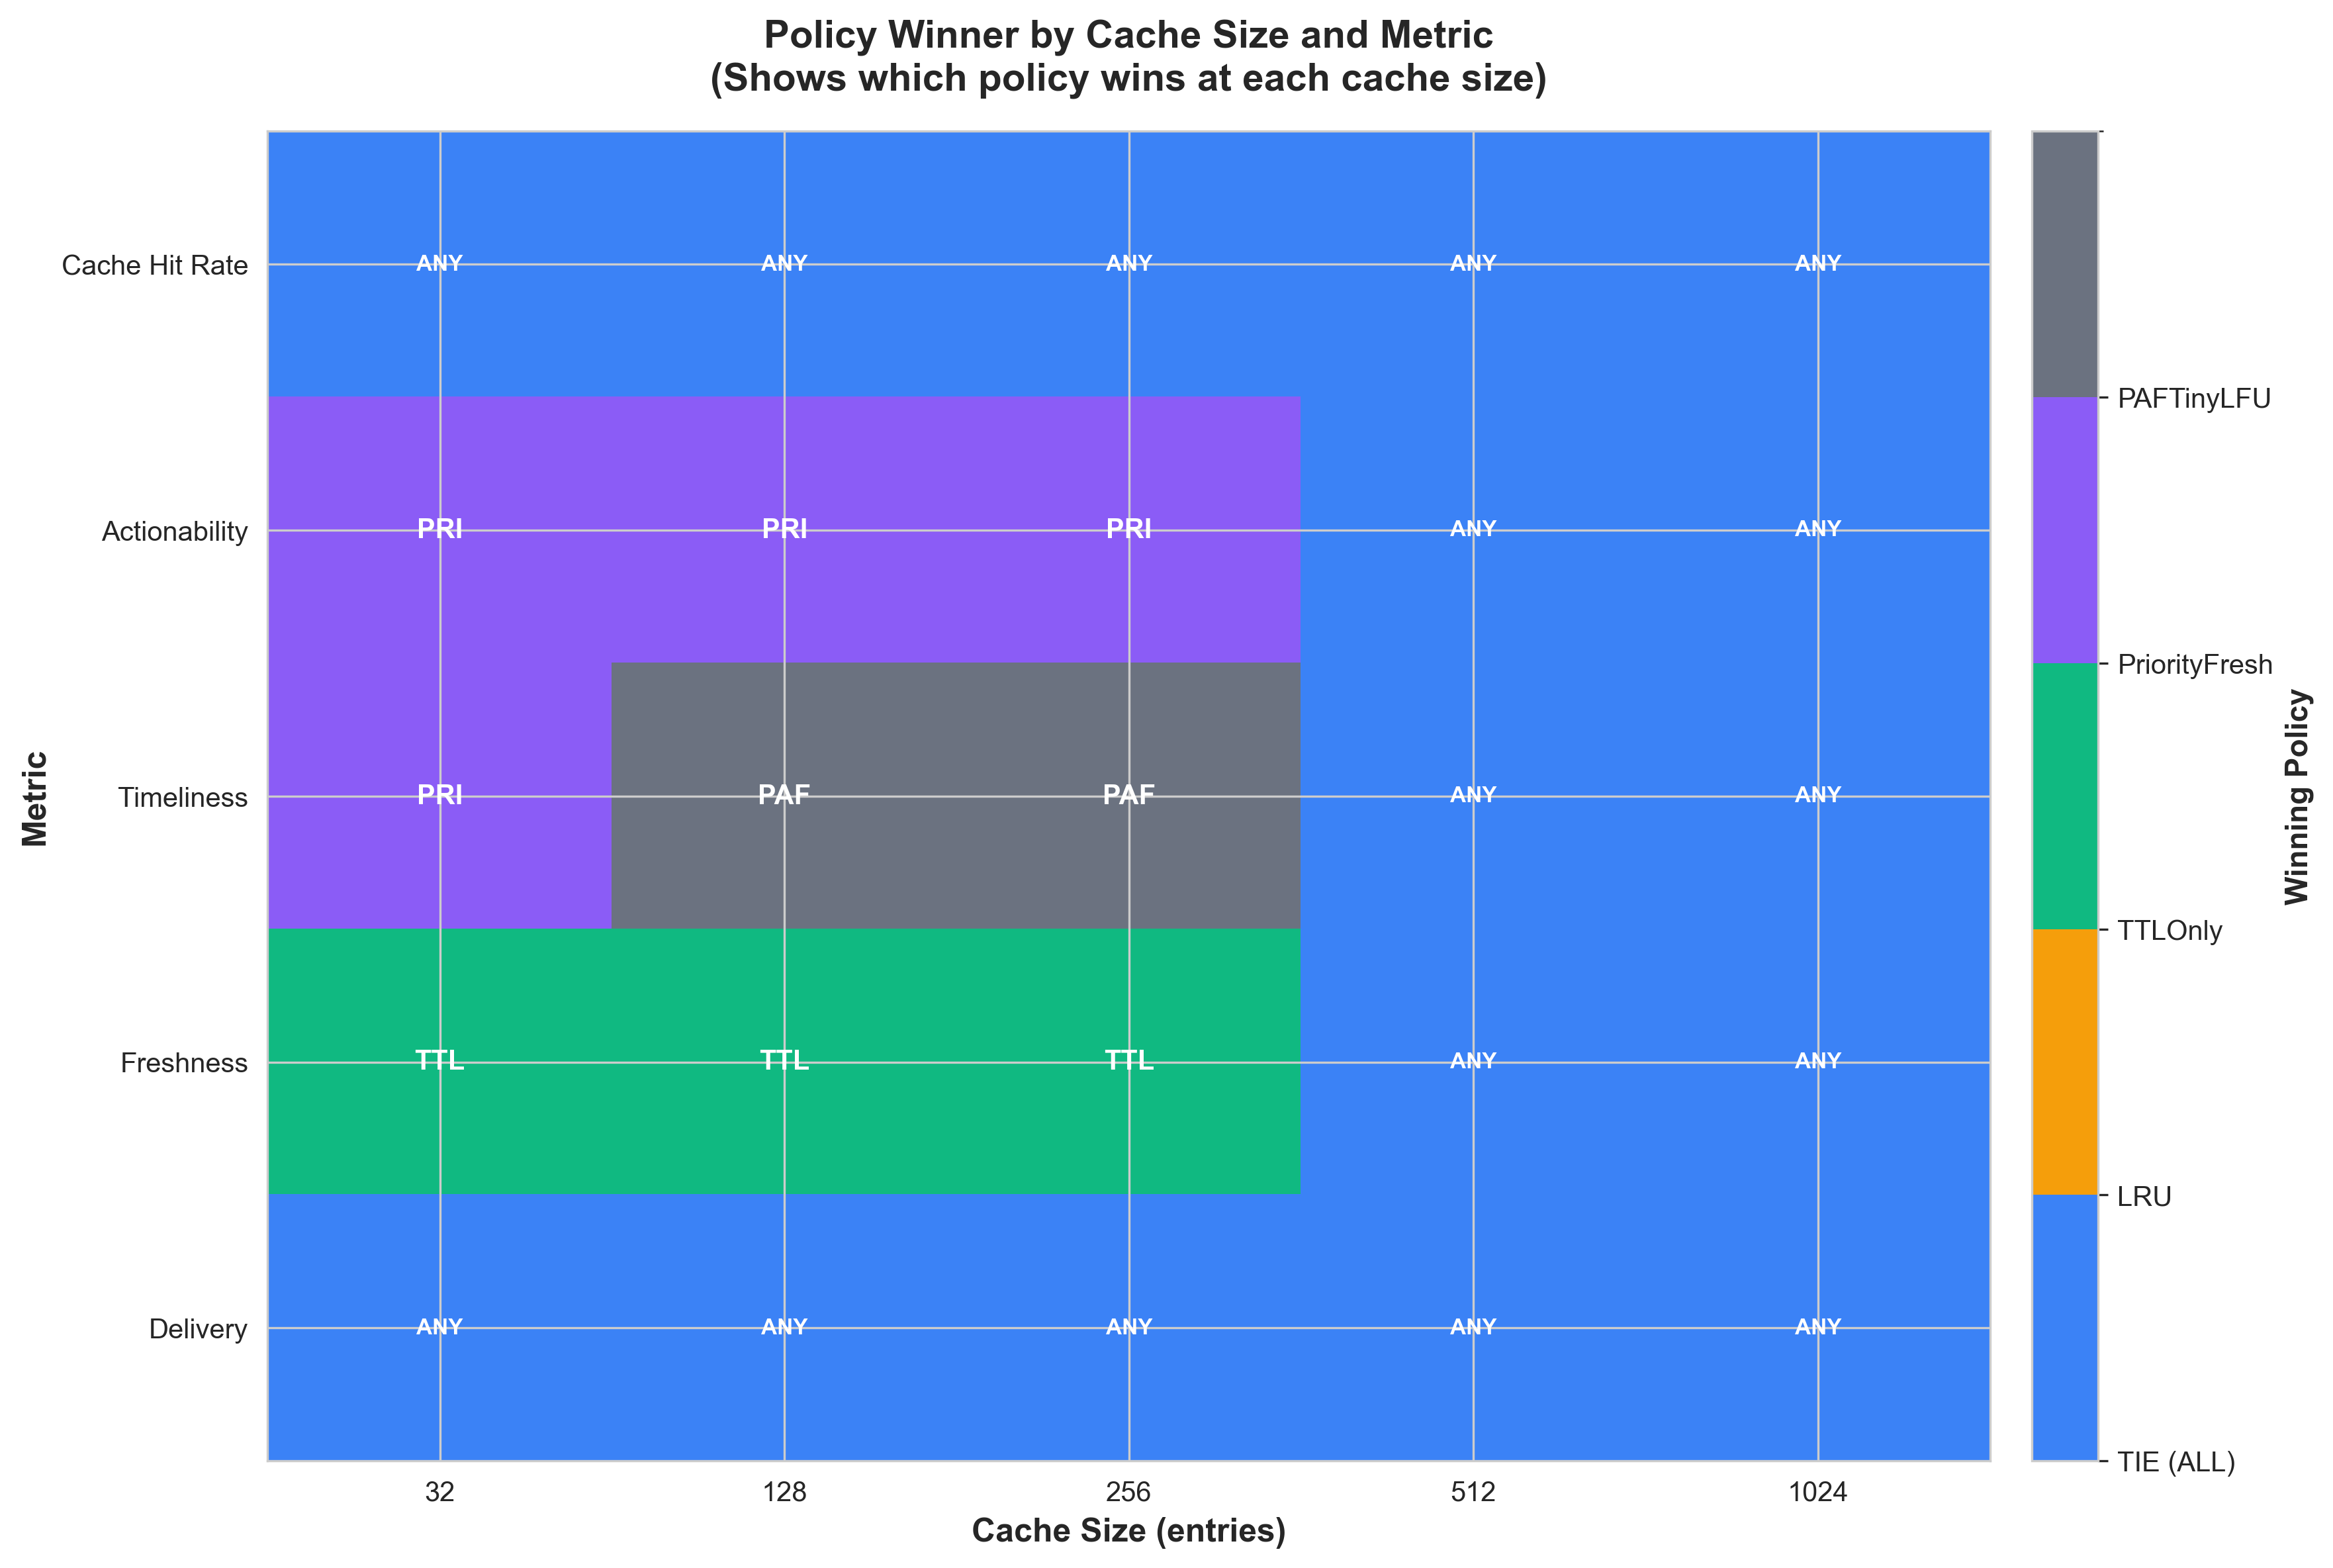
\includegraphics[width=\linewidth]{figures/device_winner_heatmap.png}
    \caption{Cache-size sweep: winner heatmap across metrics/policies.}
    \label{fig:device-winner-heatmap}
\end{figure}

\begin{figure}[h]
    \centering
    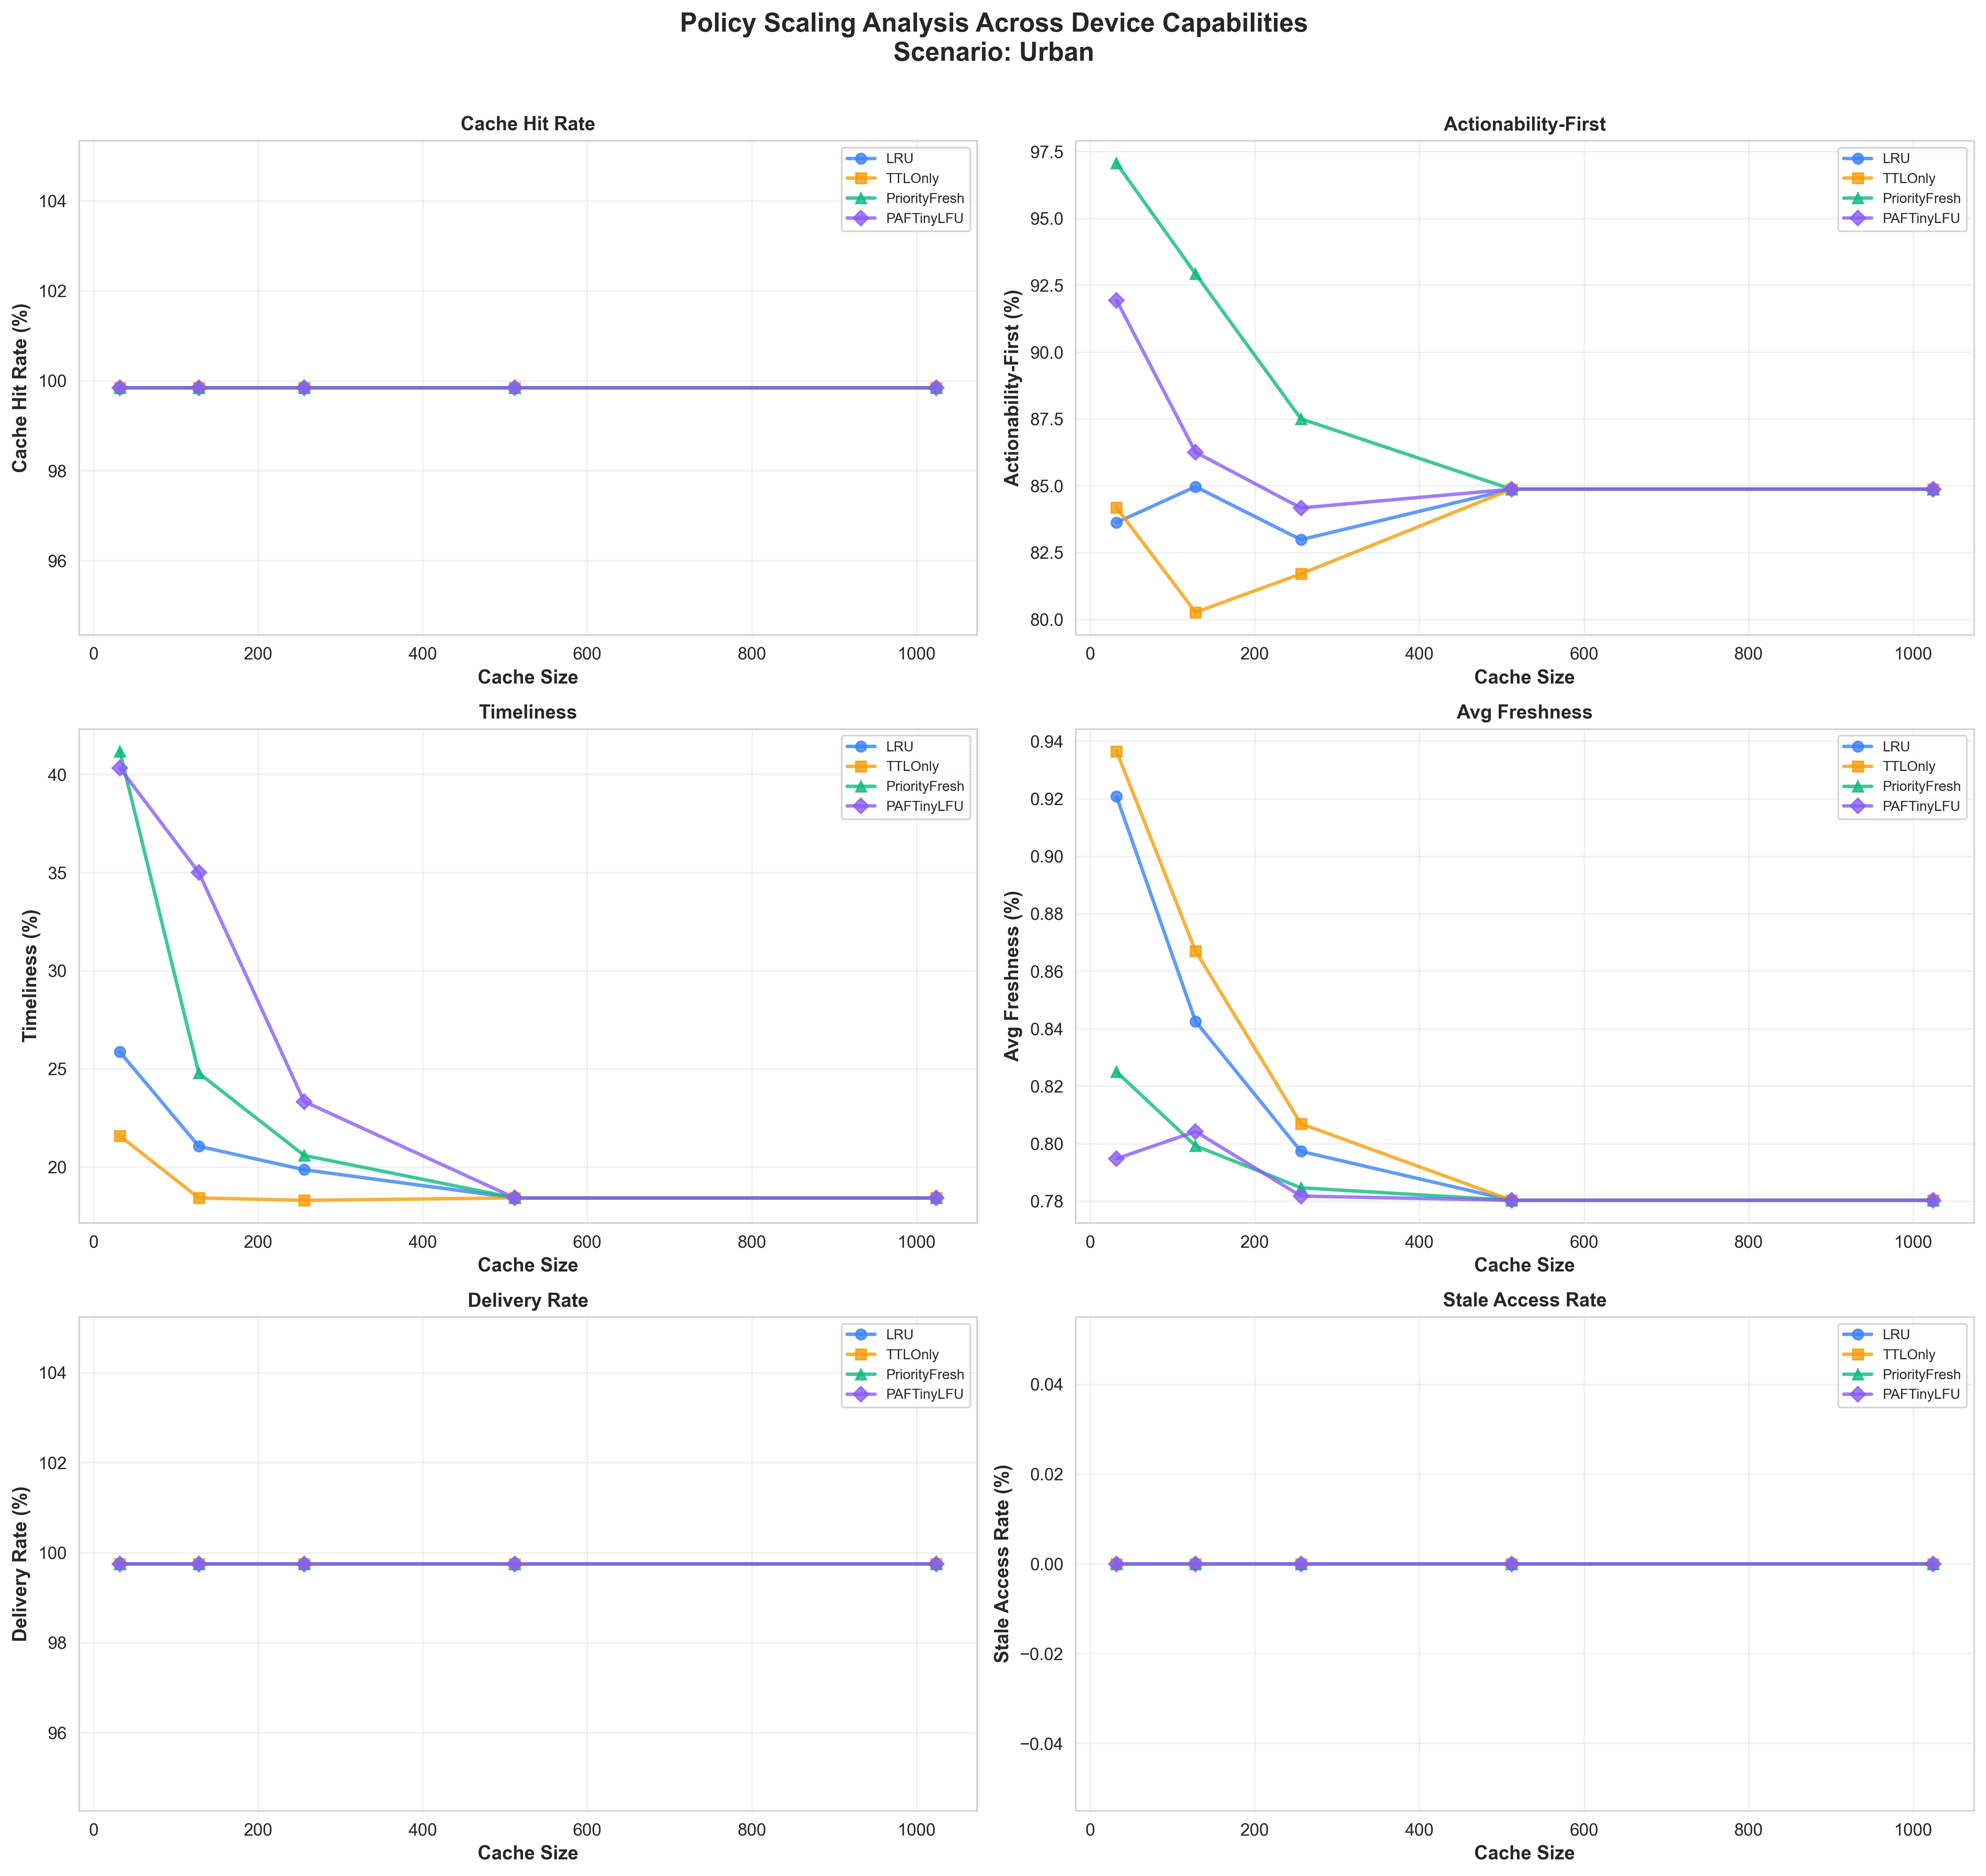
\includegraphics[width=\linewidth]{figures/device_all_metrics_grid.png}
    \caption{Cache-size sweep: all-metrics grid overview.}
    \label{fig:device-all-grid}
\end{figure}

\subsubsection{Network-reliability sweep}
\begin{figure}[h]
    \centering
    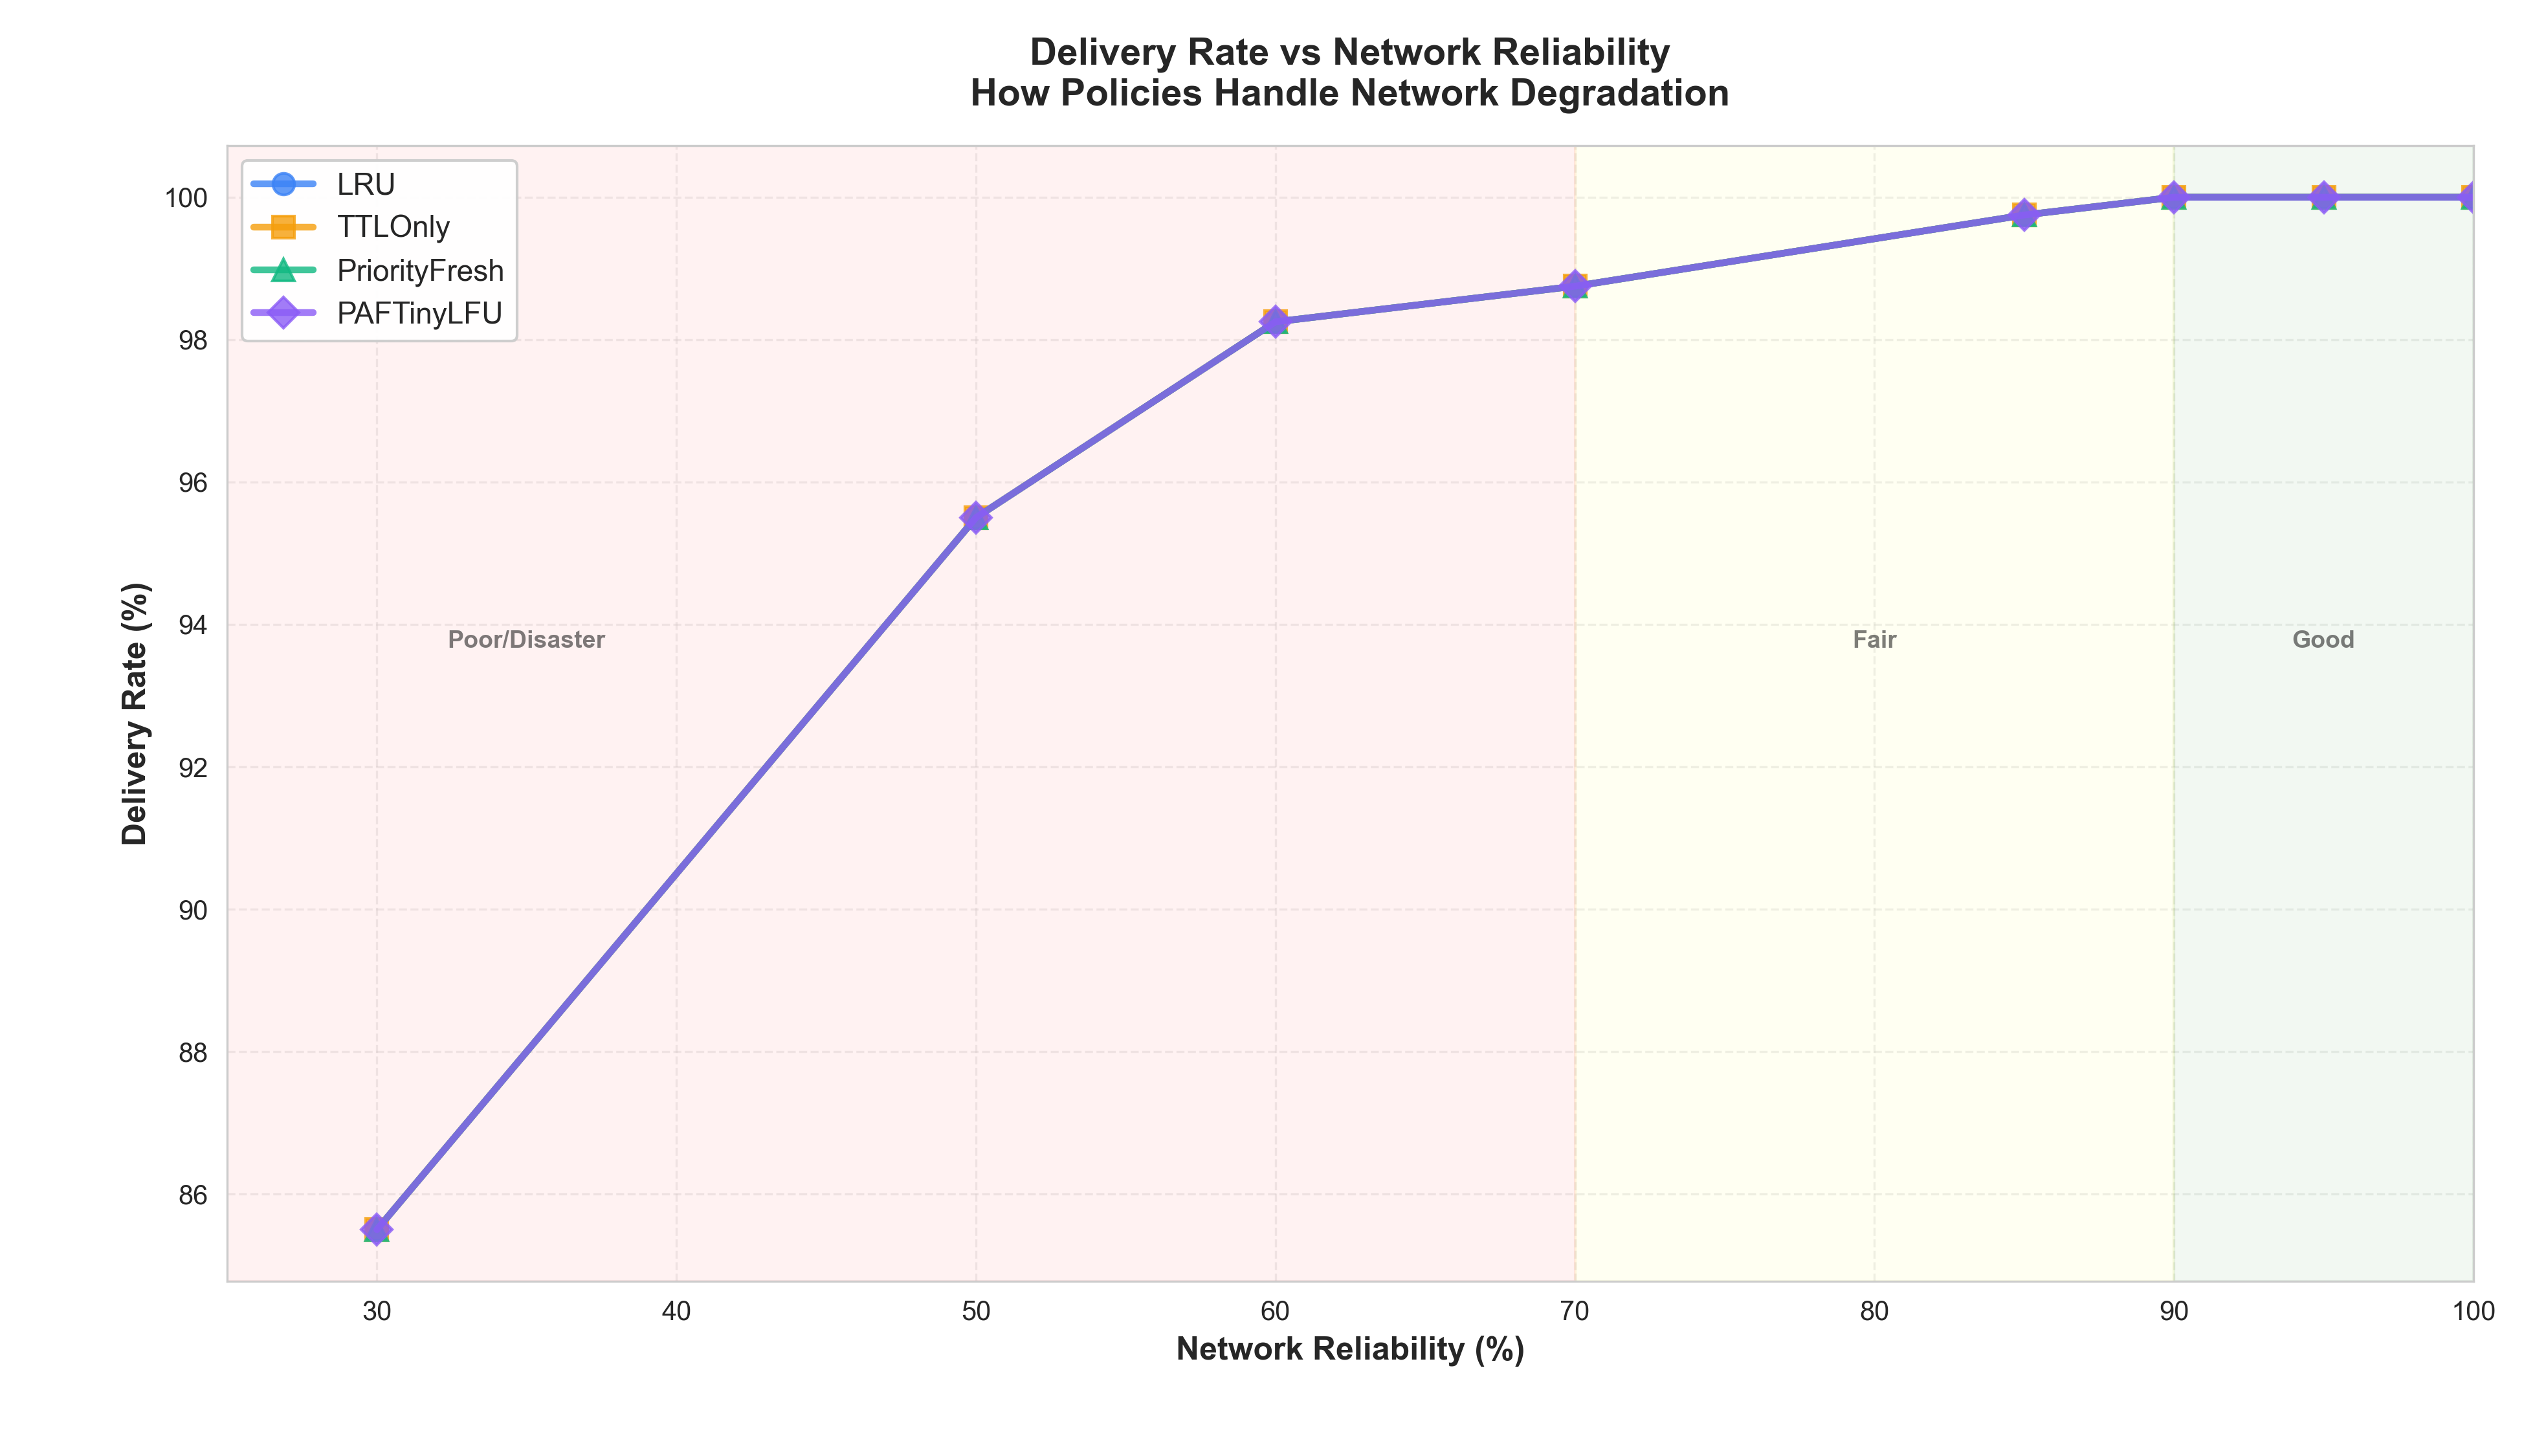
\includegraphics[width=\linewidth]{figures/network_reliability_deliveryRate.png}
    \caption{Network-reliability sweep: delivery rate across policies.}
    \label{fig:network-delivery}
\end{figure}

\begin{figure}[h]
    \centering
    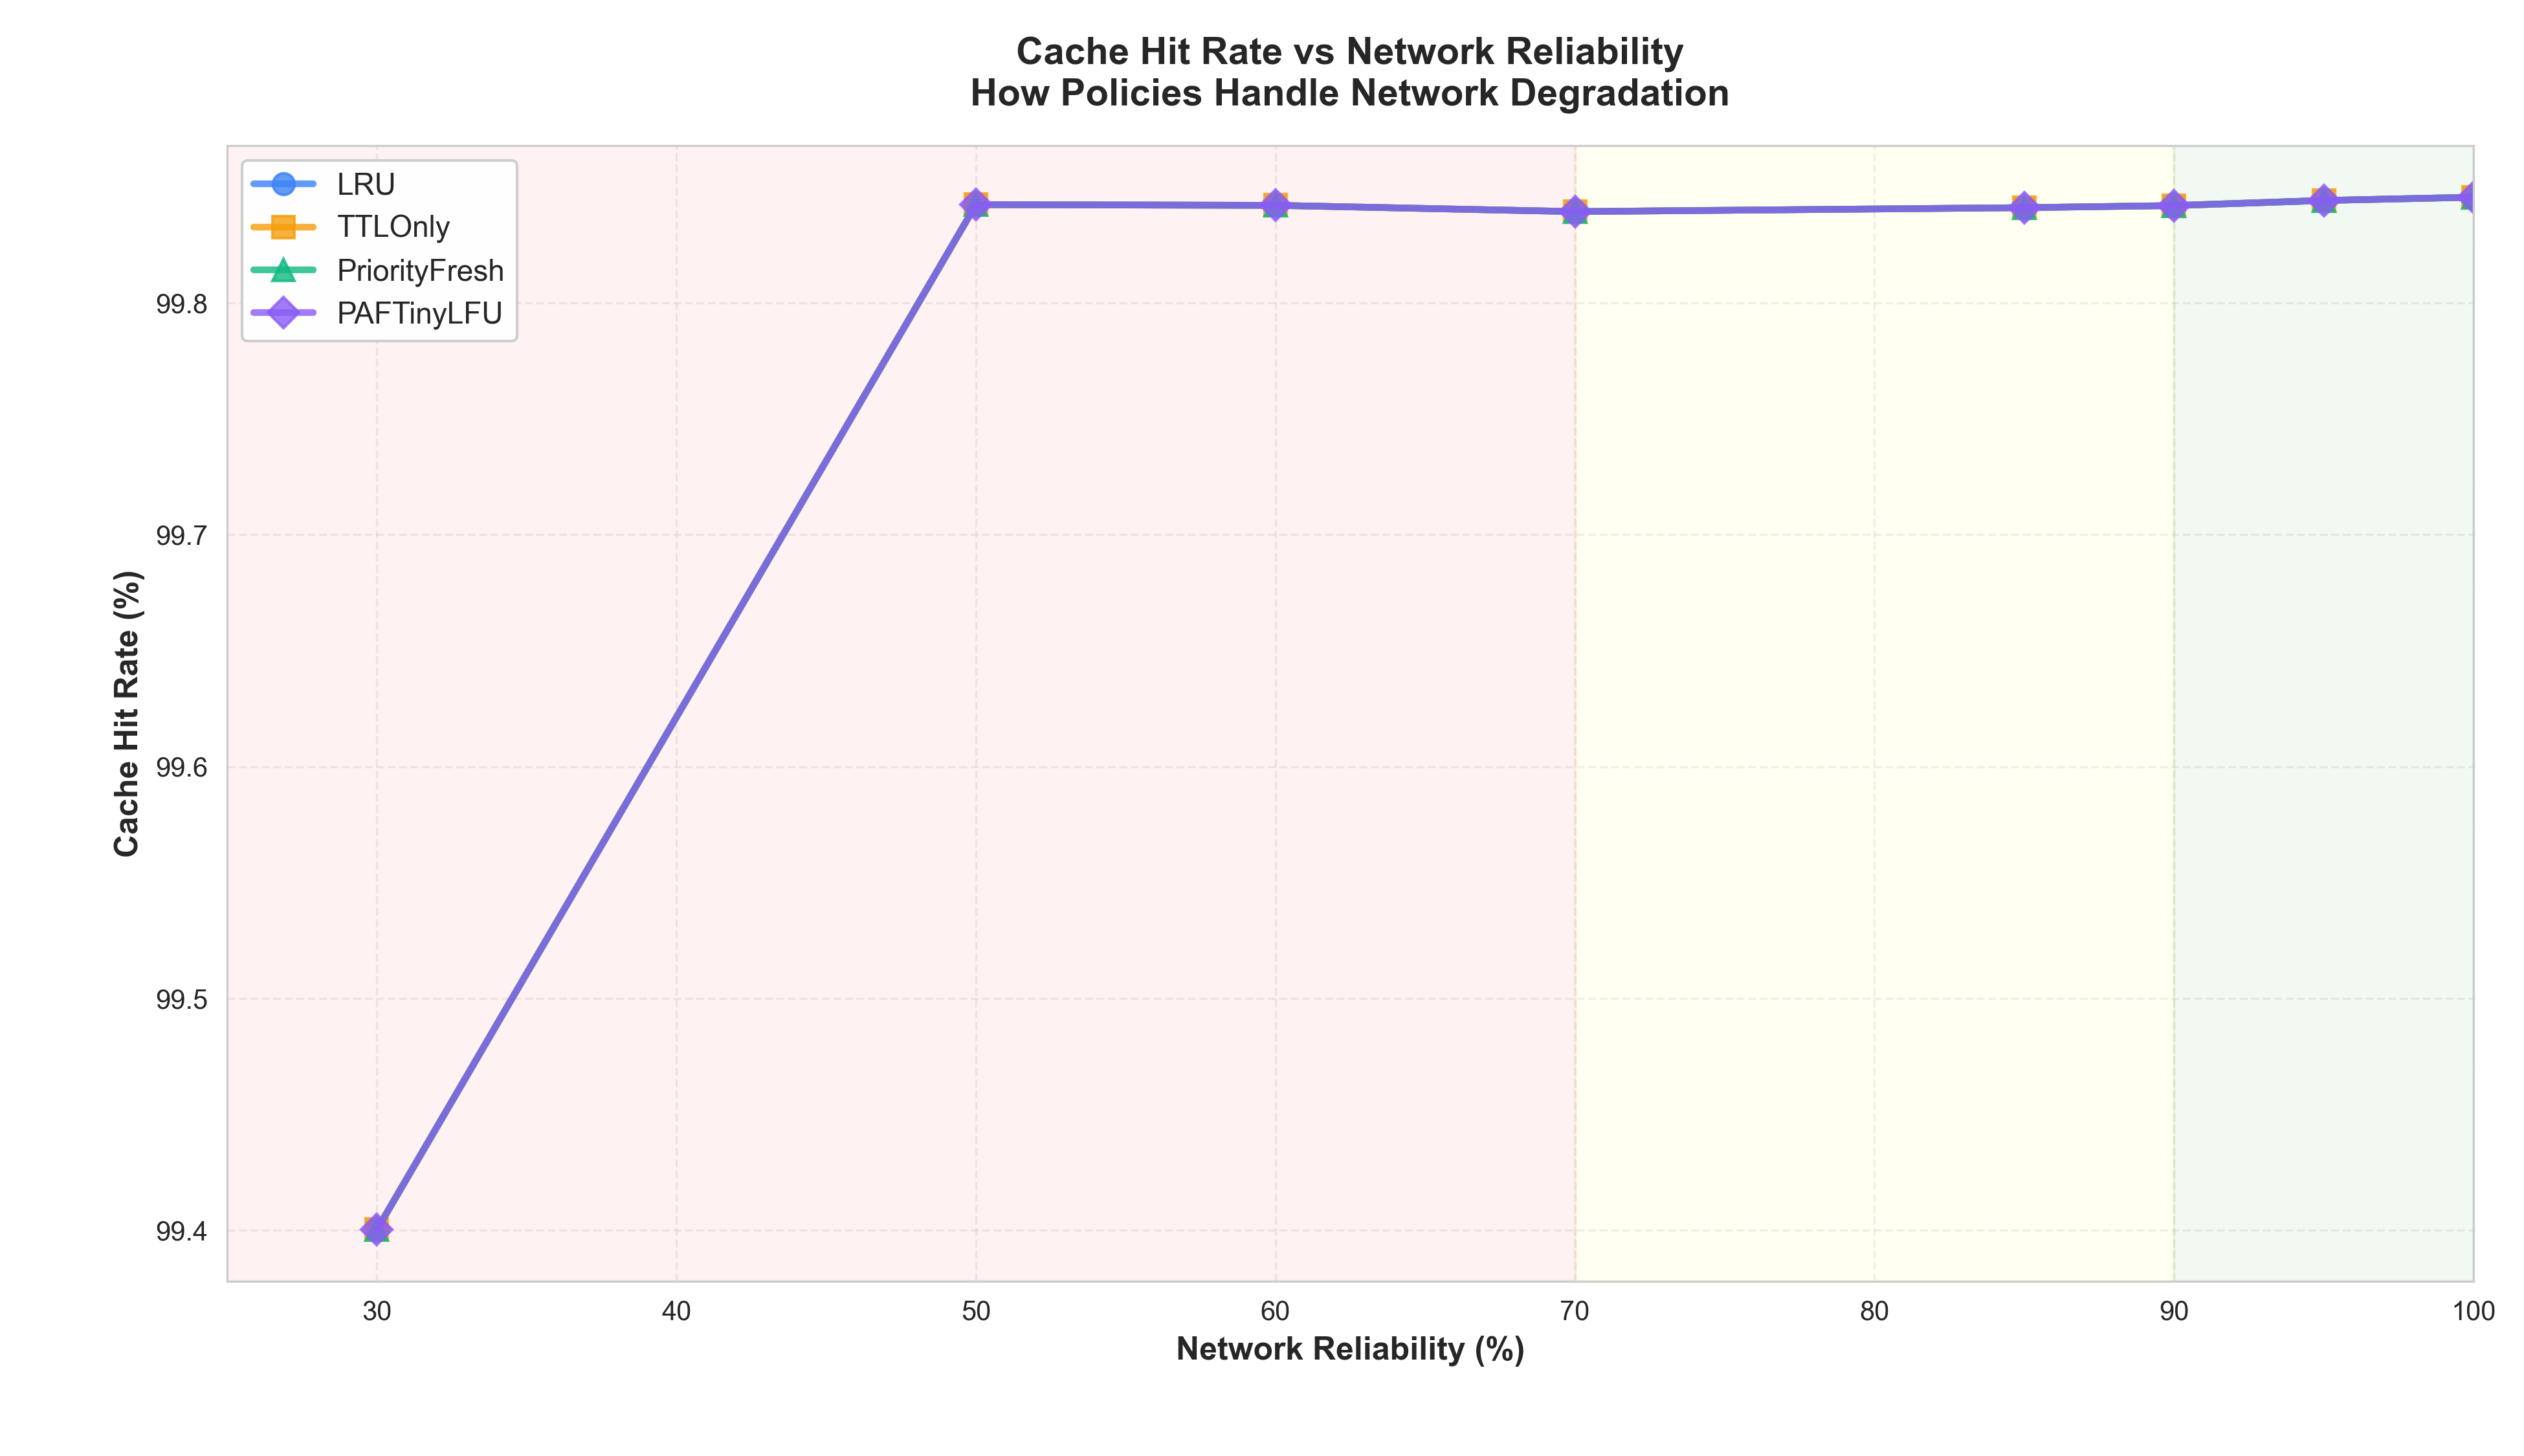
\includegraphics[width=\linewidth]{figures/network_reliability_cacheHitRate.png}
    \caption{Network-reliability sweep: cache hit rate across policies.}
    \label{fig:network-cachehit}
\end{figure}

\begin{figure}[h]
    \centering
    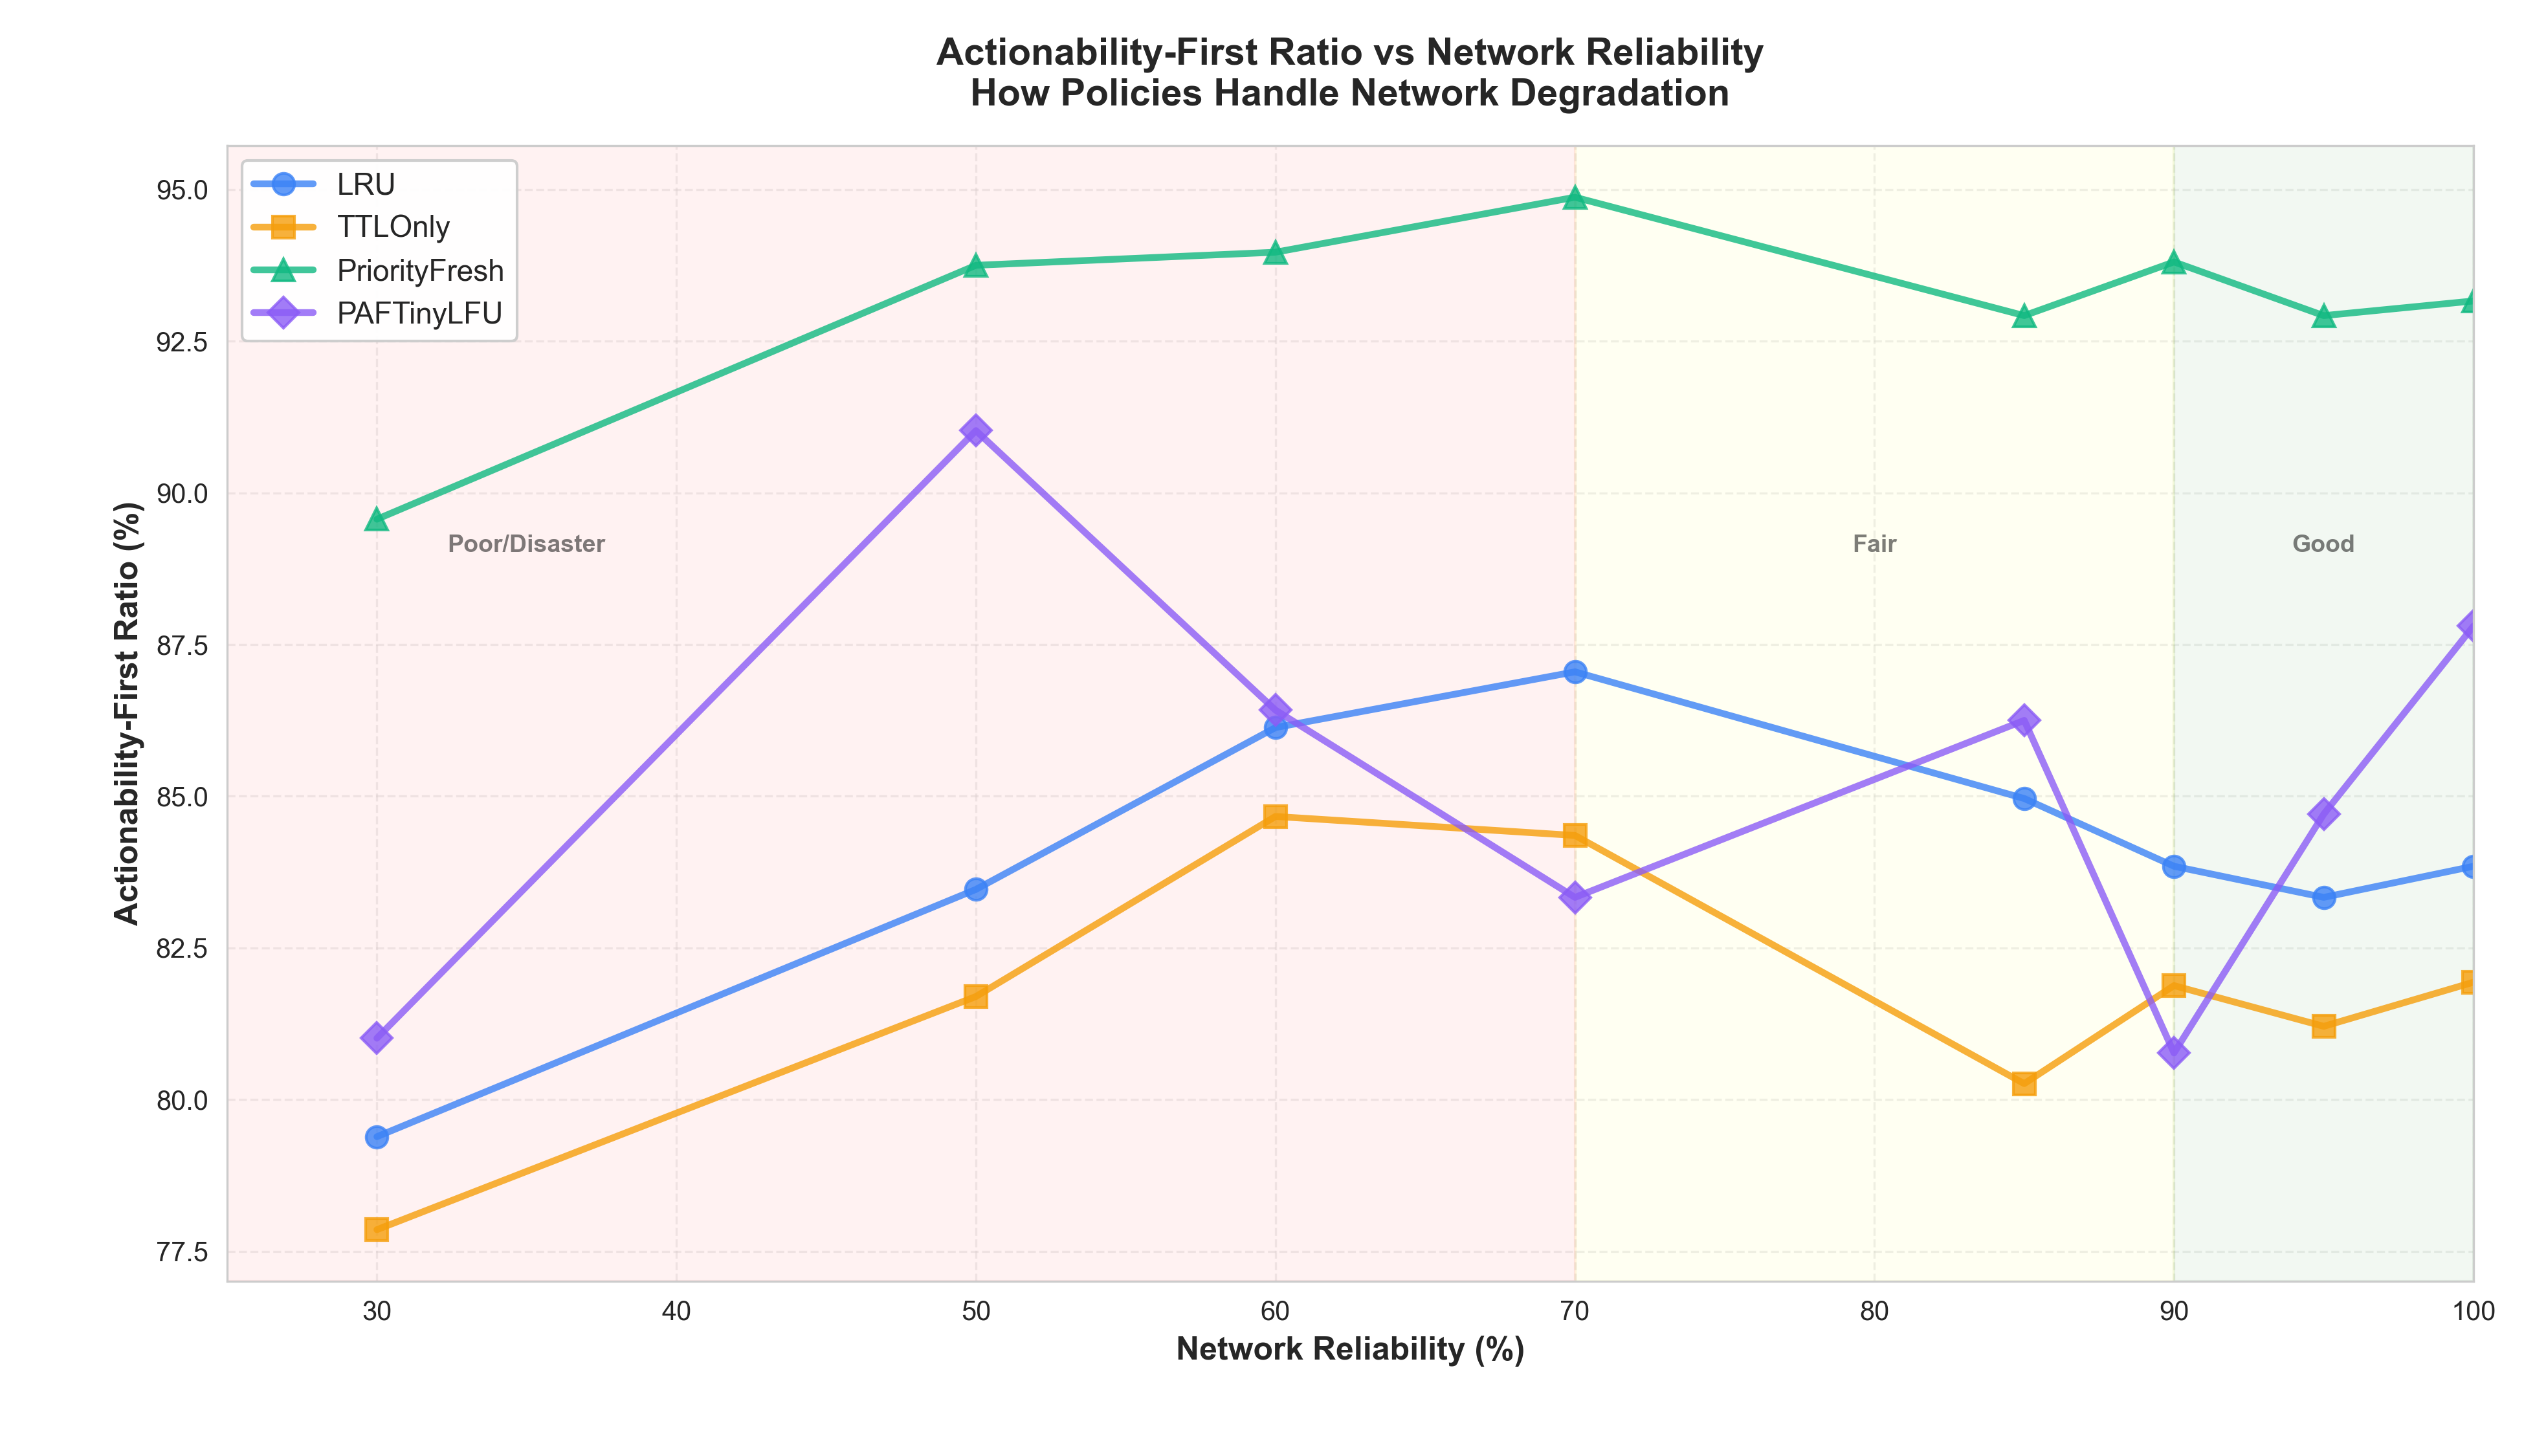
\includegraphics[width=\linewidth]{figures/network_reliability_actionabilityFirstRatio.png}
    \caption{Network-reliability sweep: actionability-first ratio across policies.}
    \label{fig:network-actionability}
\end{figure}

\begin{figure}[h]
    \centering
    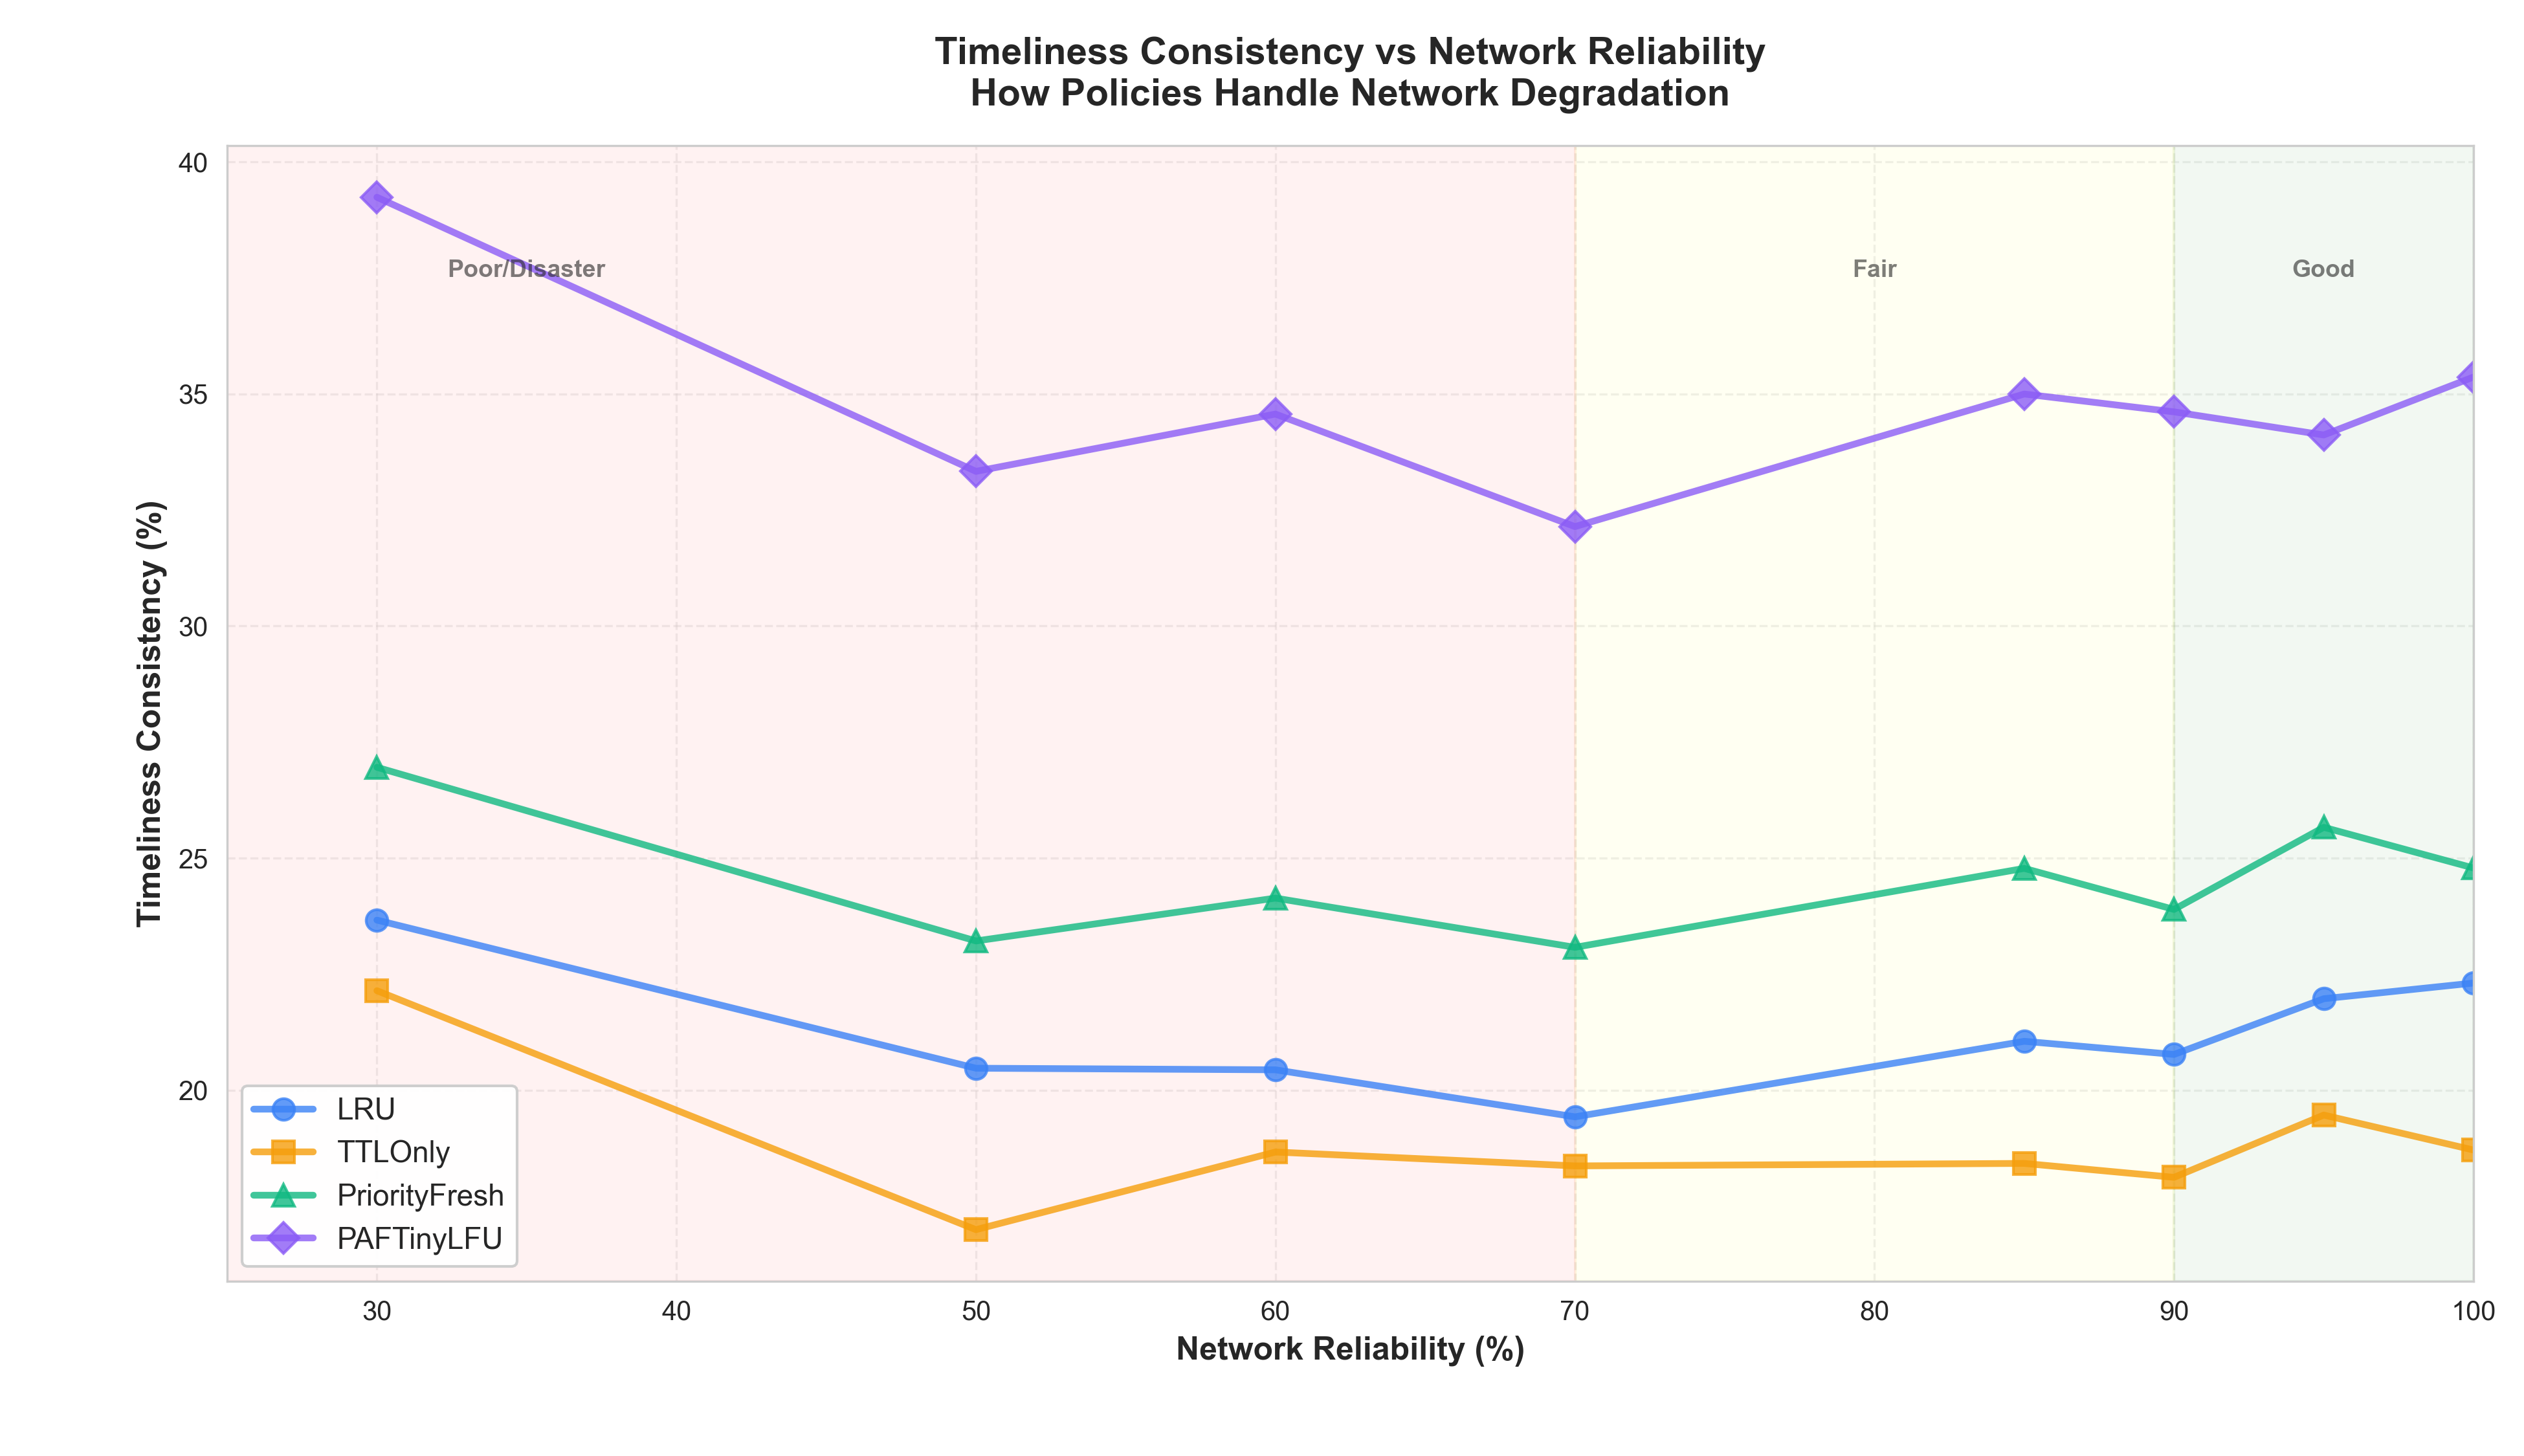
\includegraphics[width=\linewidth]{figures/network_reliability_timelinessConsistency.png}
    \caption{Network-reliability sweep: timeliness consistency across policies.}
    \label{fig:network-timeliness}
\end{figure}

\begin{figure}[h]
    \centering
    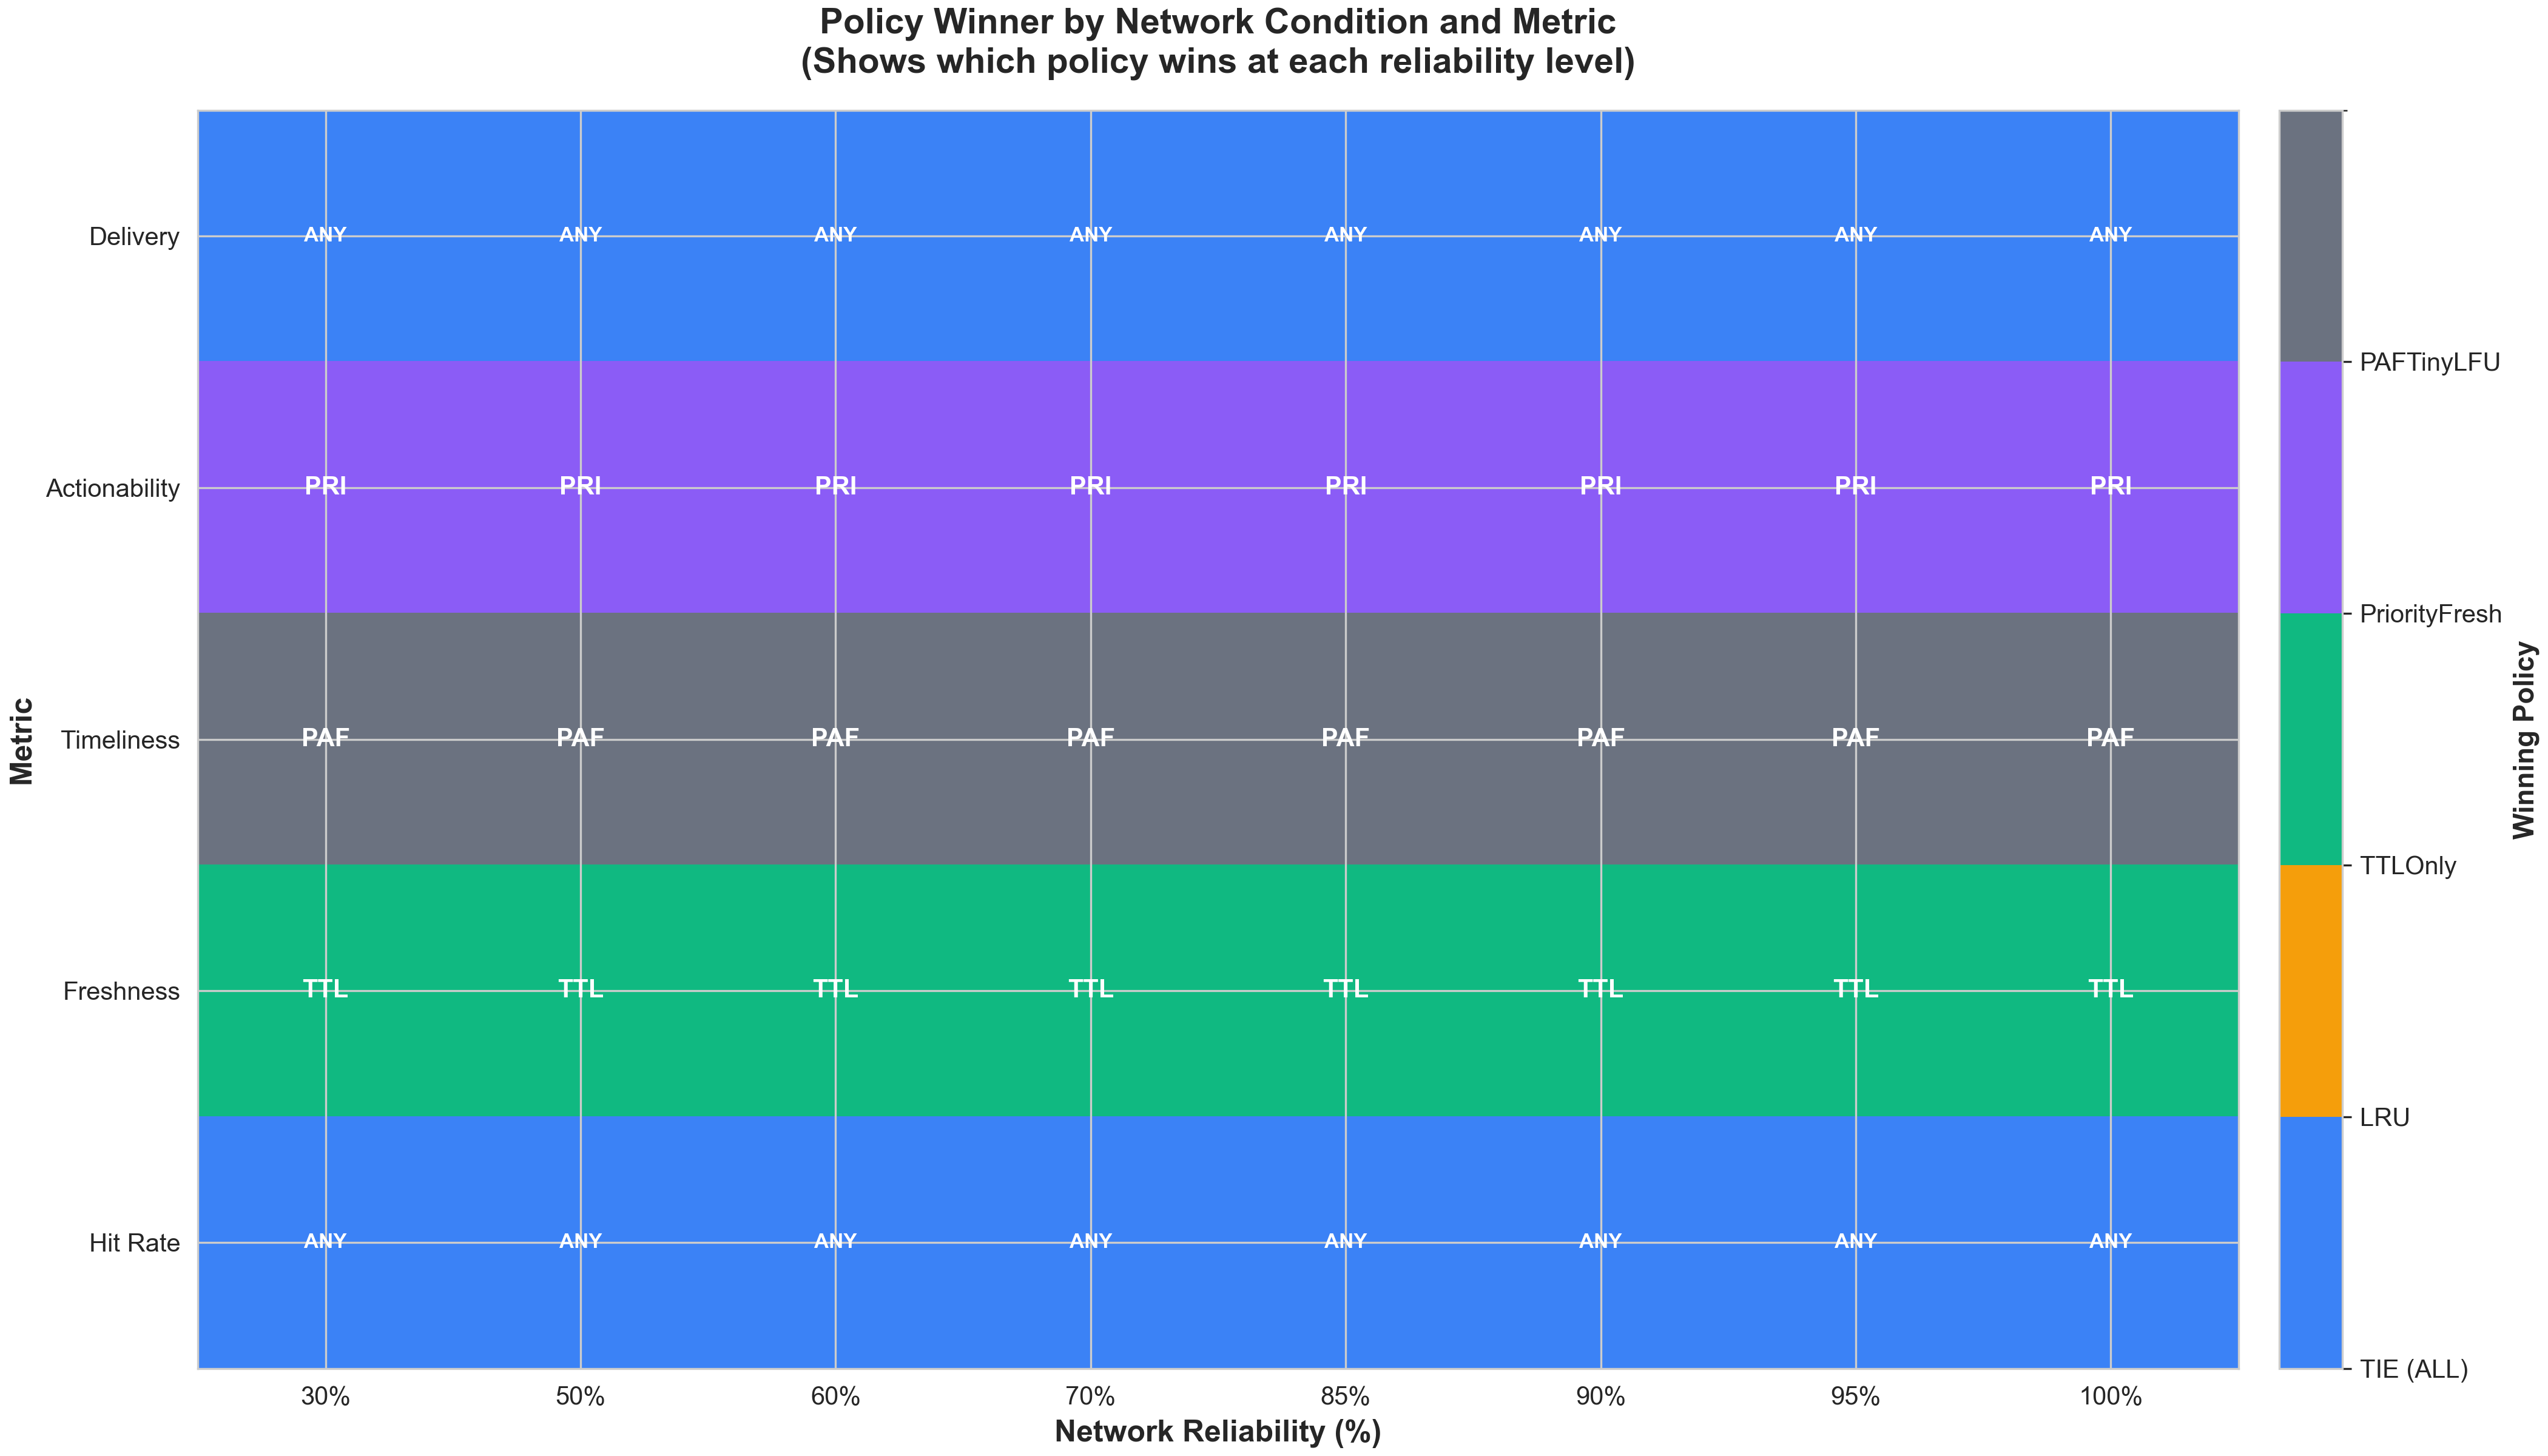
\includegraphics[width=\linewidth]{figures/network_winner_heatmap.png}
    \caption{Network-reliability sweep: winner heatmap across metrics/policies.}
    \label{fig:network-winner-heatmap}
\end{figure}

\begin{figure}[h]
    \centering
    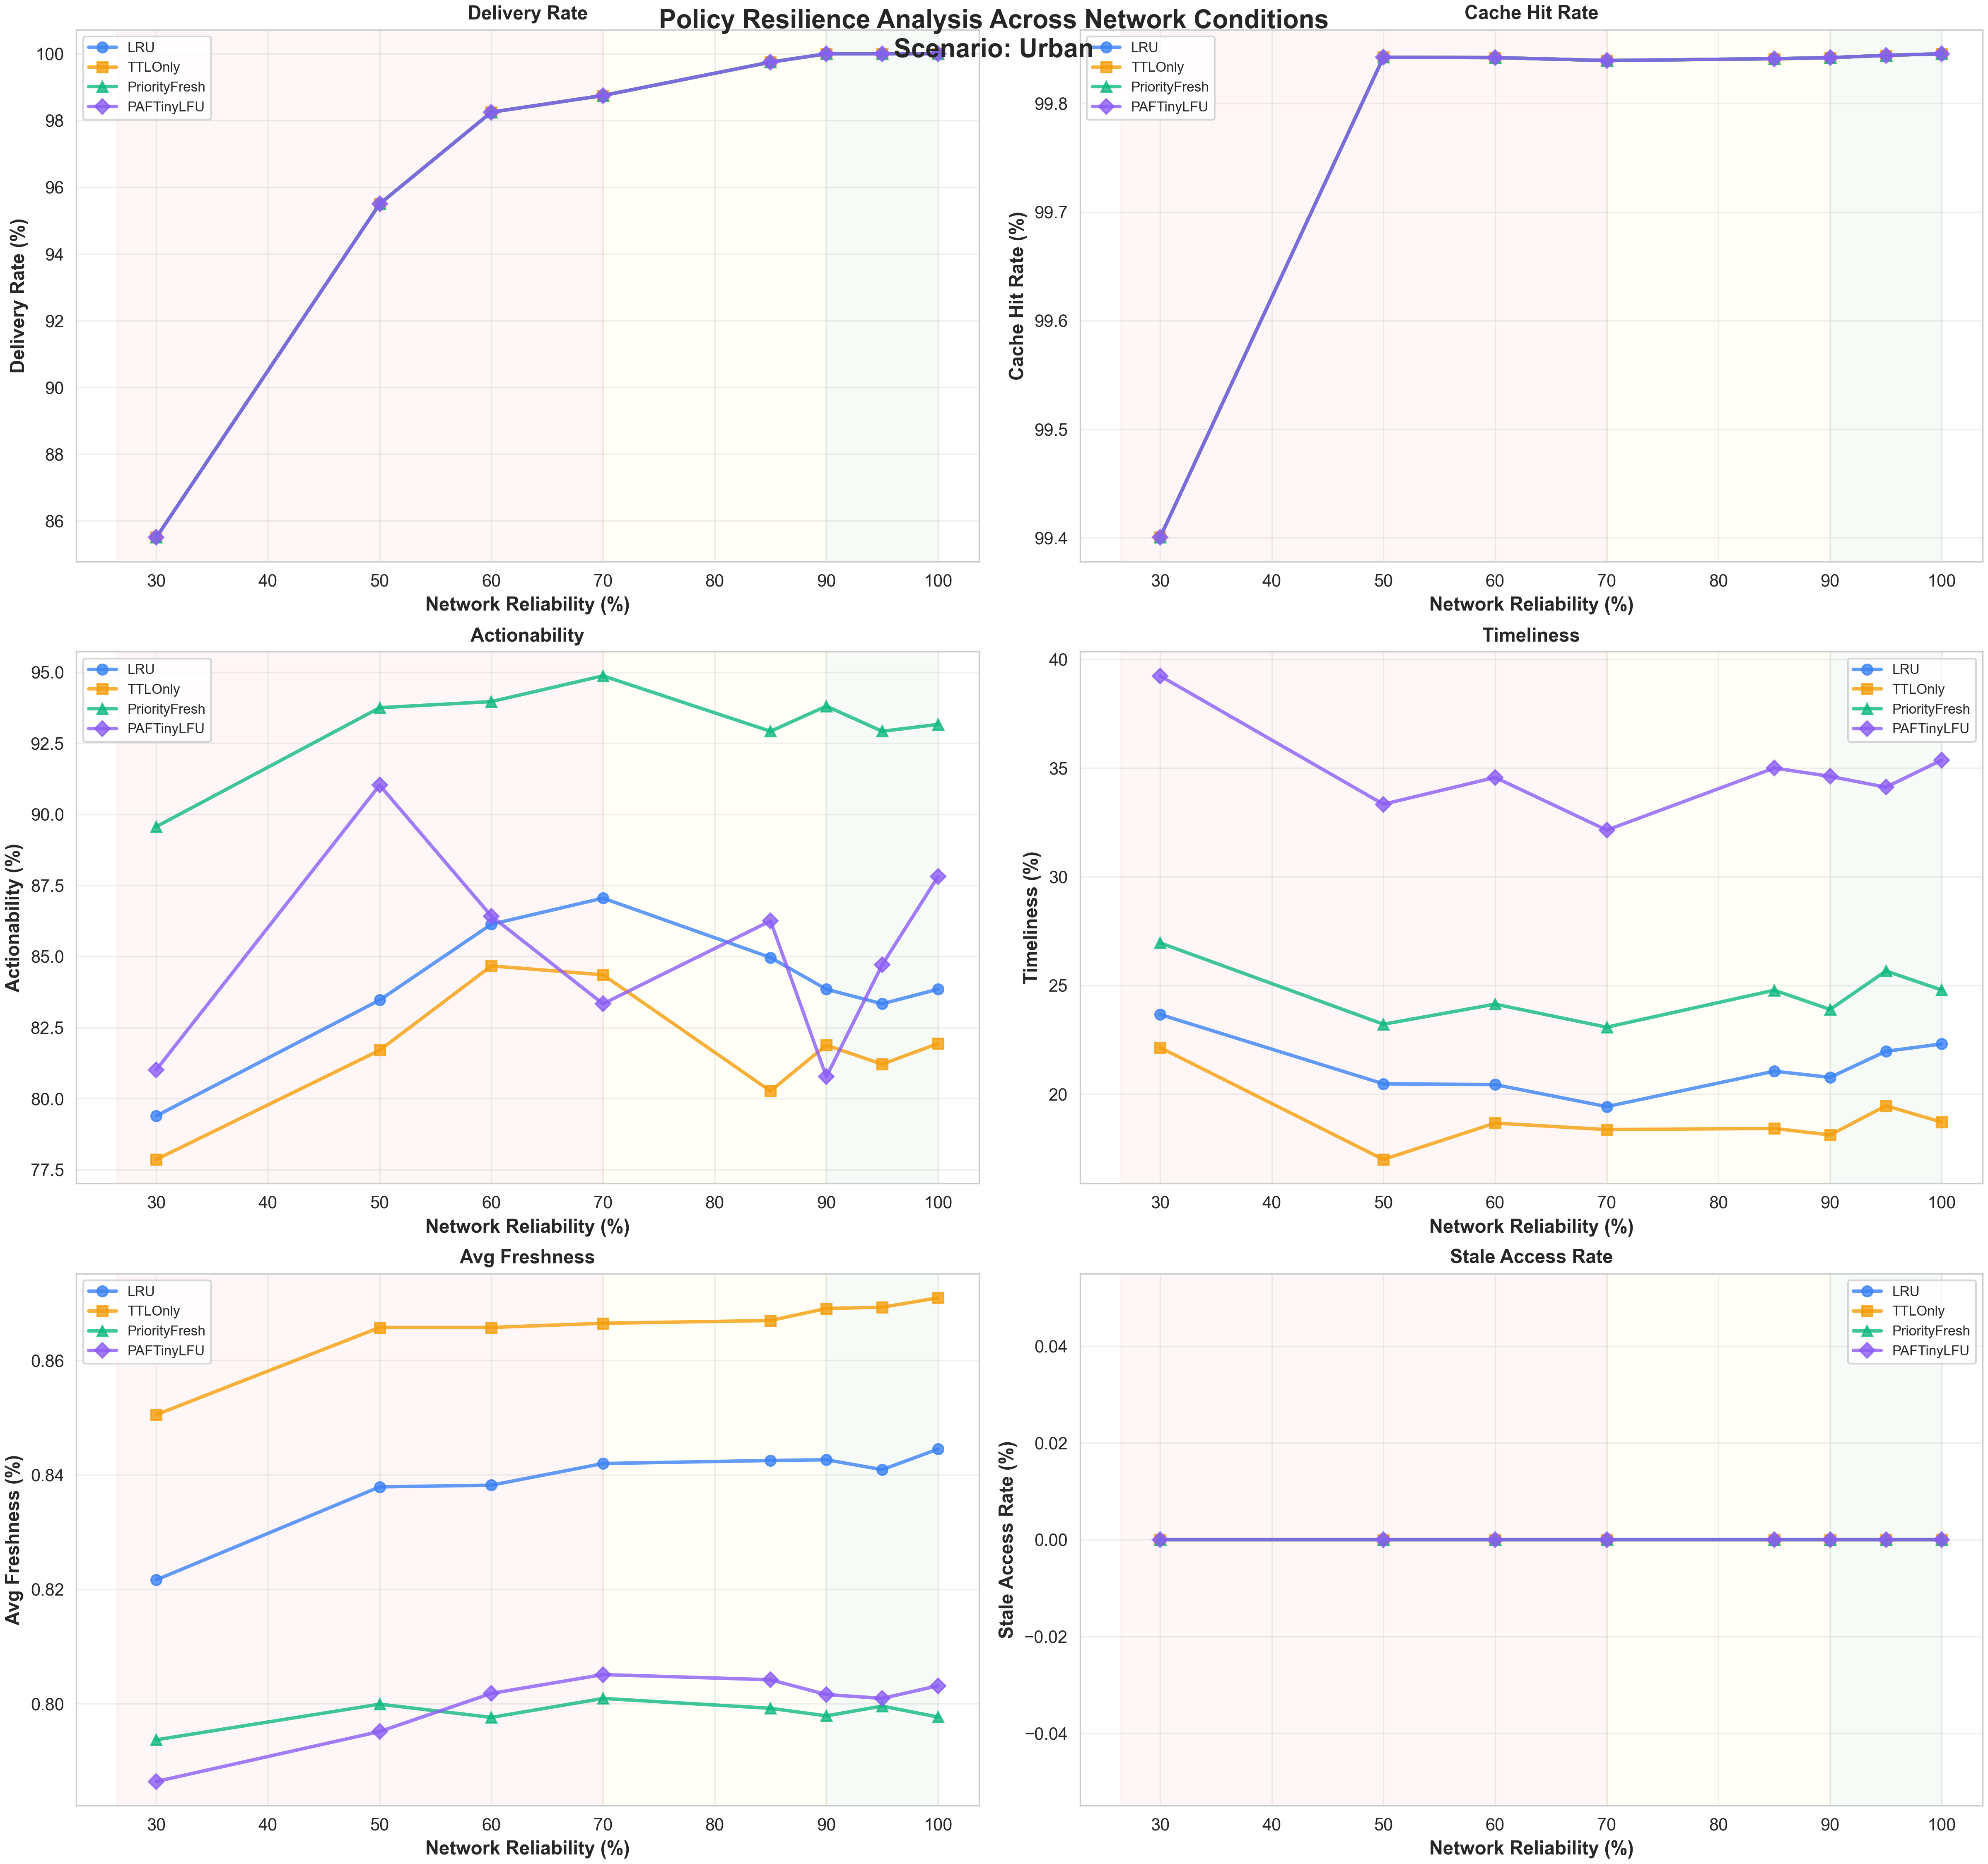
\includegraphics[width=\linewidth]{figures/network_all_metrics_grid.png}
    \caption{Network-reliability sweep: all-metrics grid overview.}
    \label{fig:network-all-grid}
\end{figure}

\subsubsection{Joint sweep: cache size and network}
\begin{figure}[h]
    \centering
    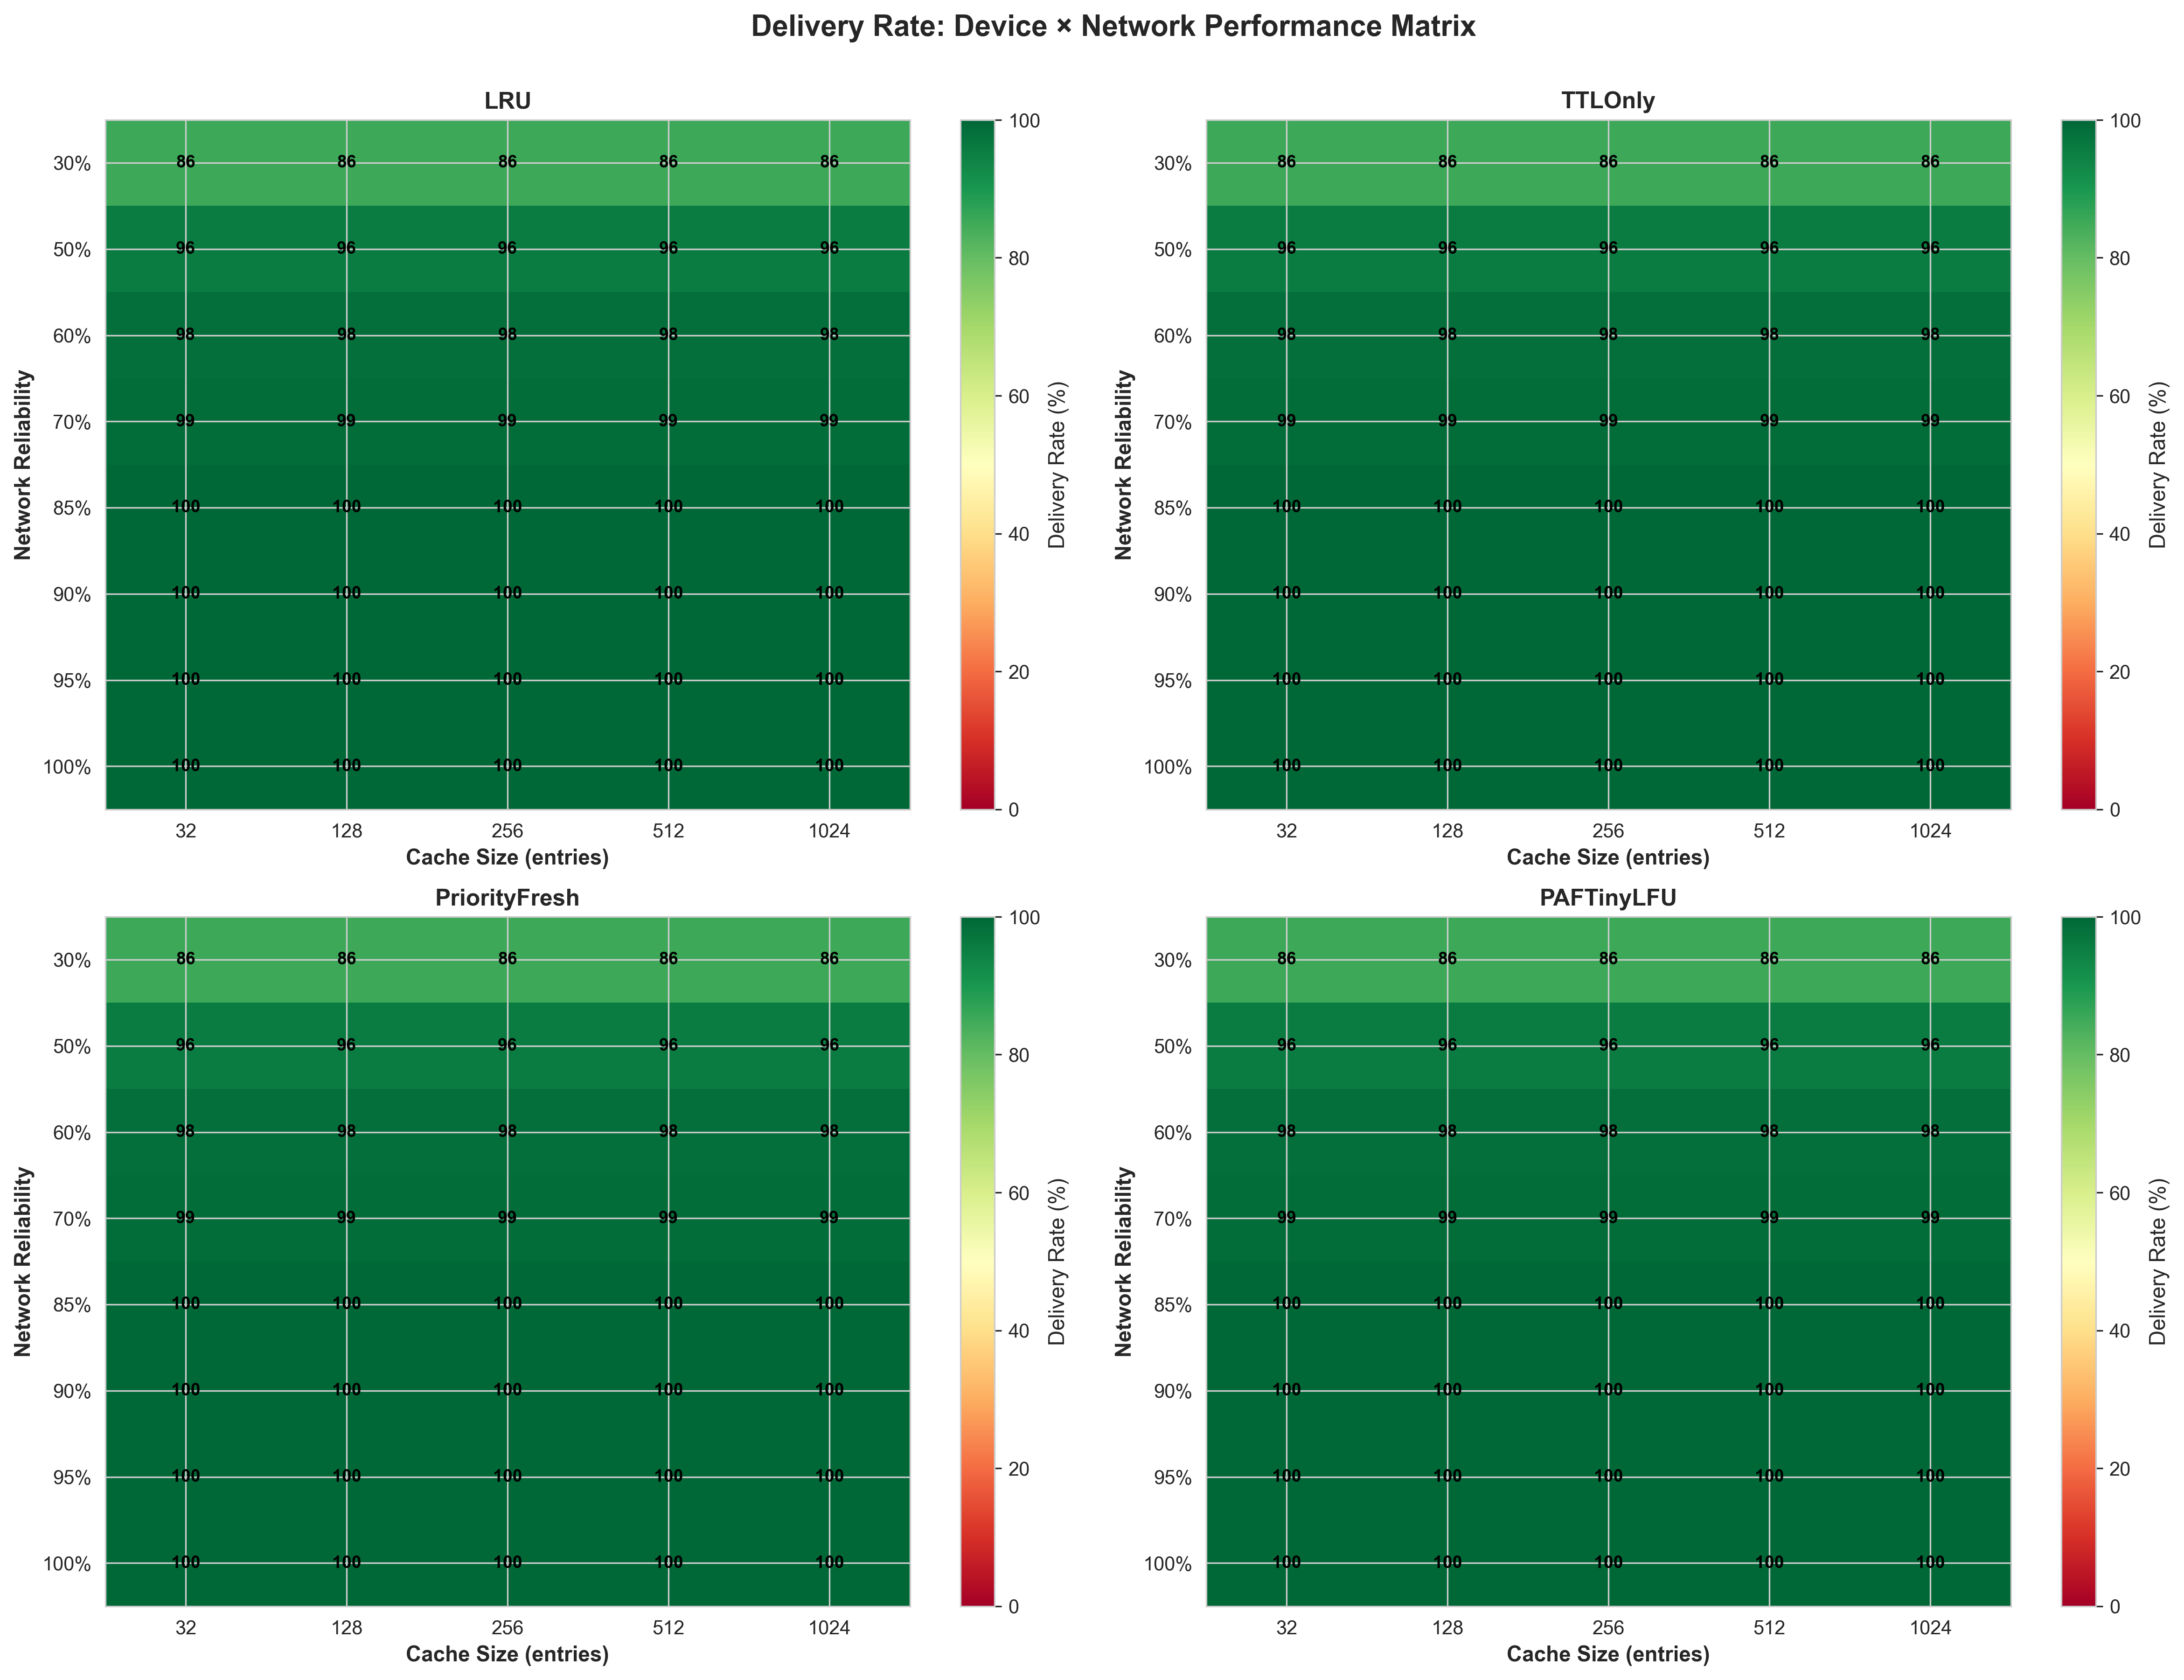
\includegraphics[width=\linewidth]{figures/combined_heatmap_matrix_deliveryRate.png}
    \caption{Joint sweep (cache size \& network): delivery rate heatmap matrix.}
    \label{fig:combined-heatmap-delivery}
\end{figure}

\begin{figure}[h]
    \centering
    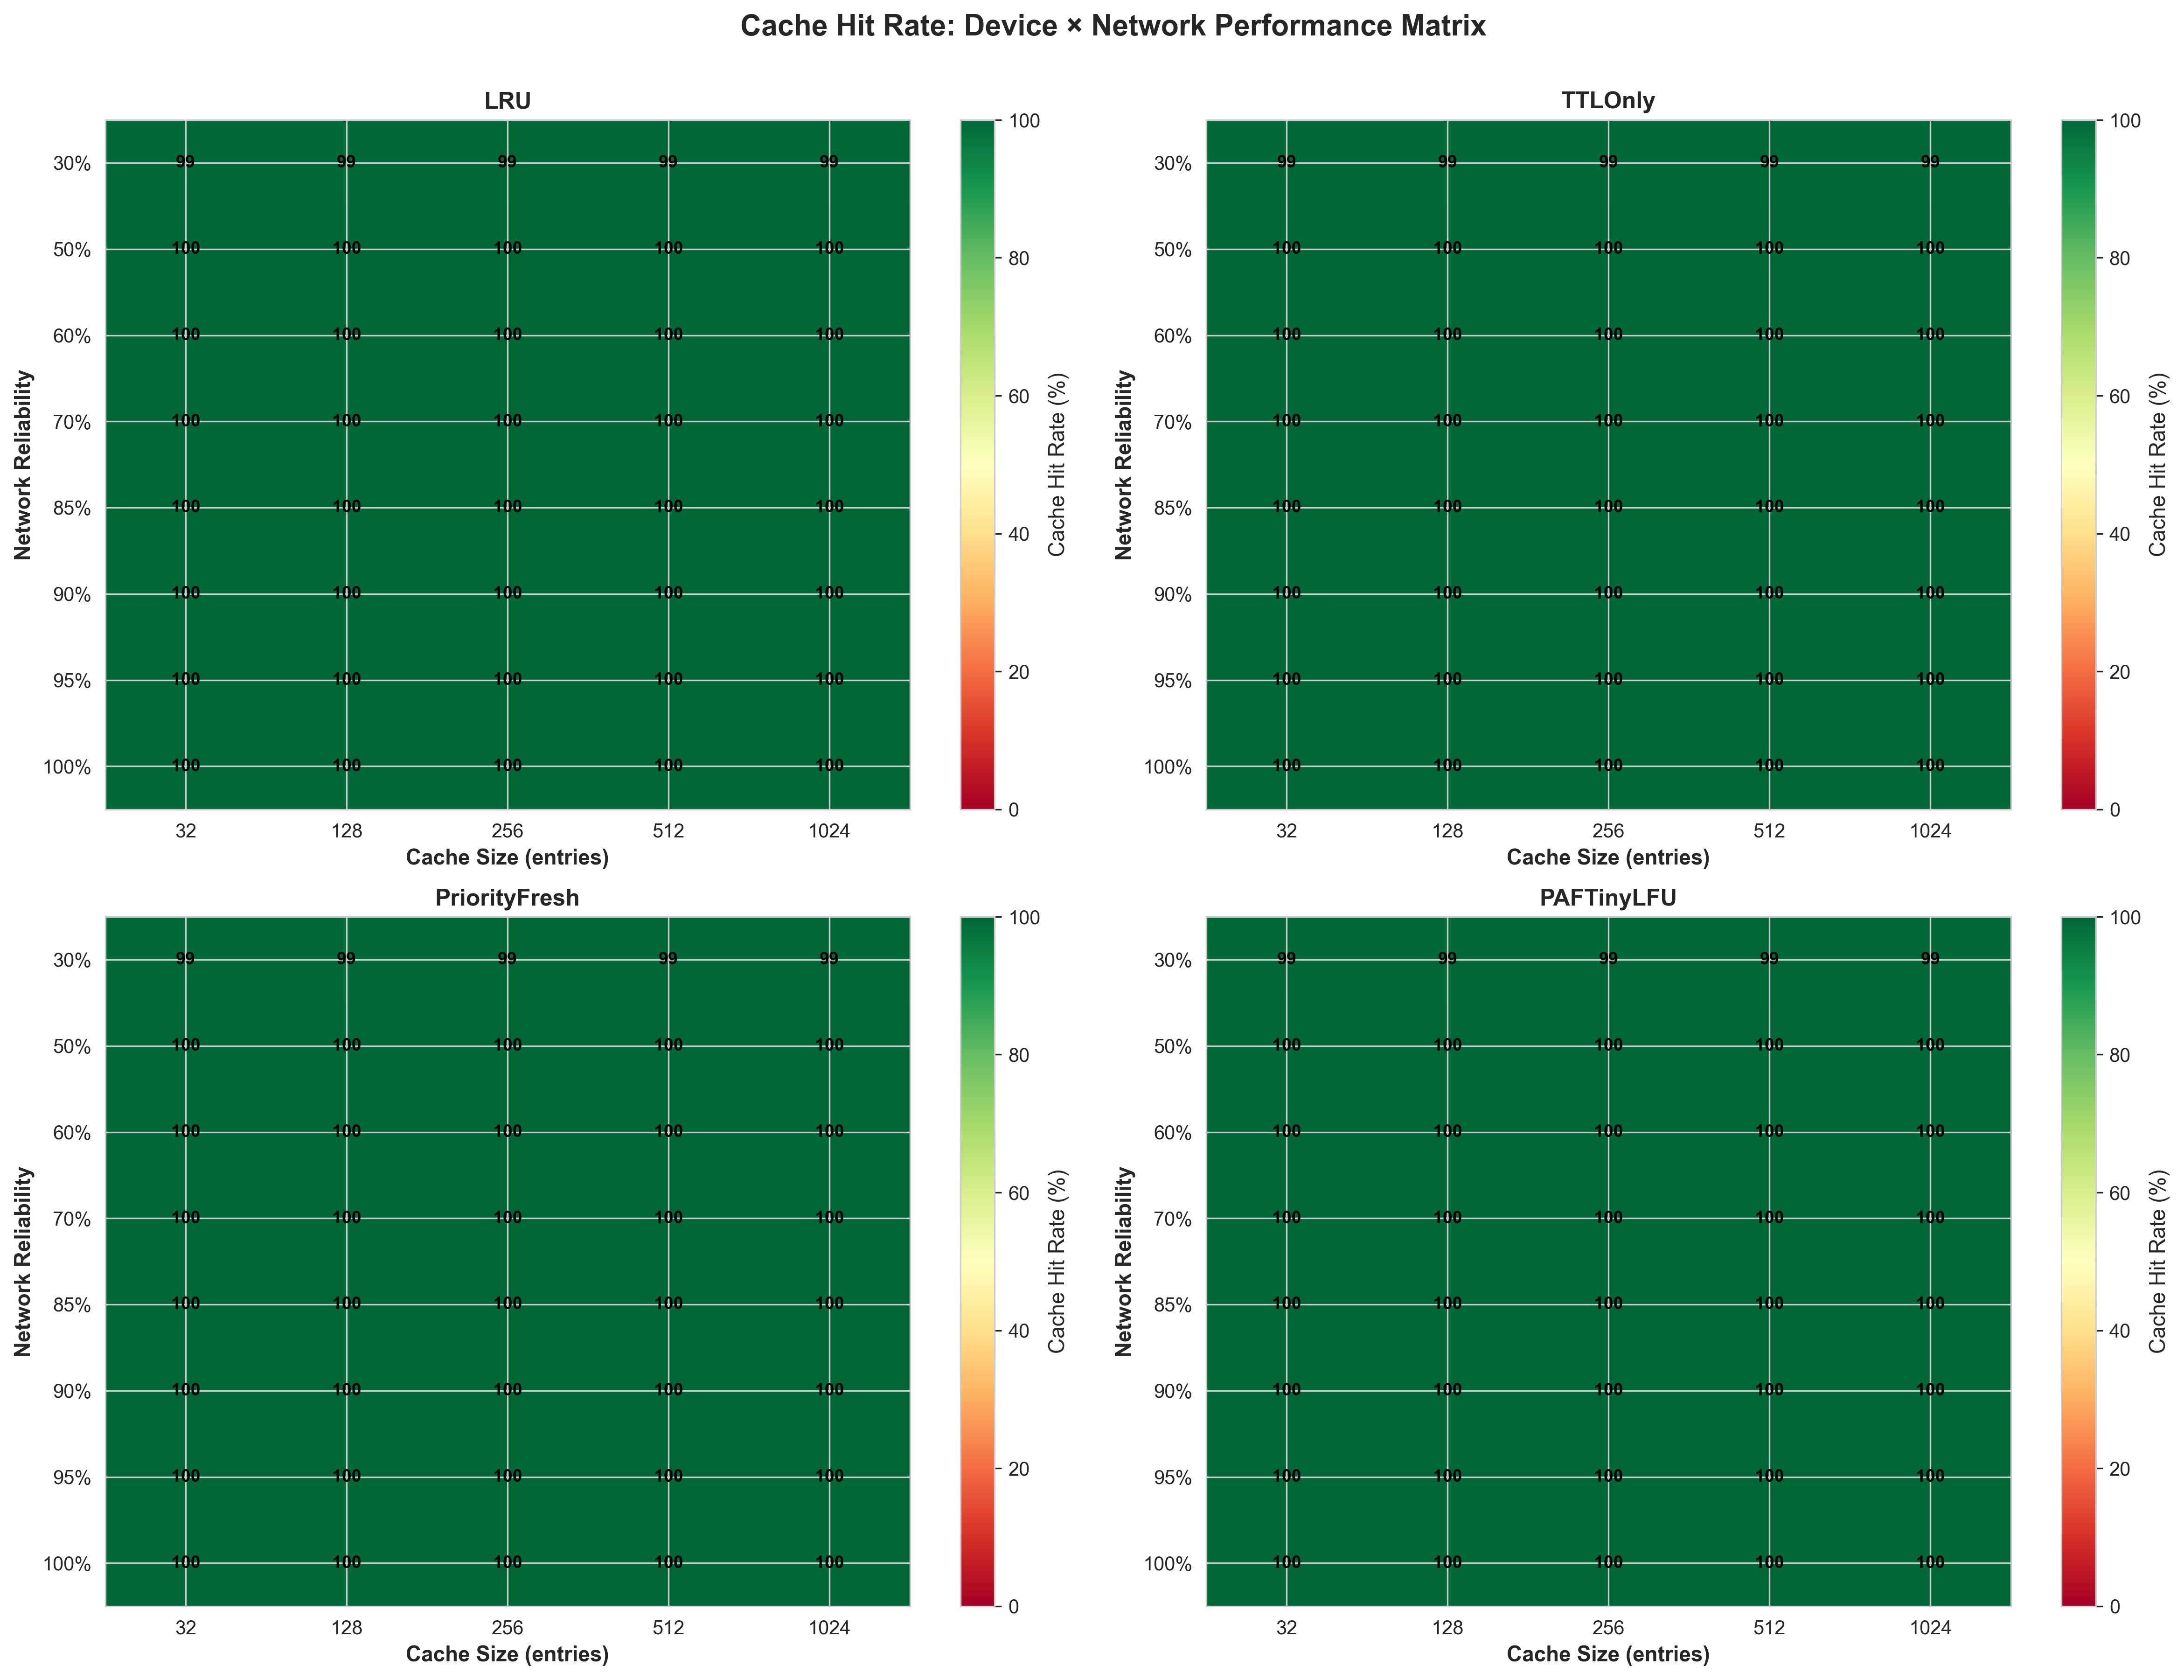
\includegraphics[width=\linewidth]{figures/combined_heatmap_matrix_cacheHitRate.png}
    \caption{Joint sweep: cache hit rate heatmap matrix.}
    \label{fig:combined-heatmap-cachehit}
\end{figure}

\begin{figure}[h]
    \centering
    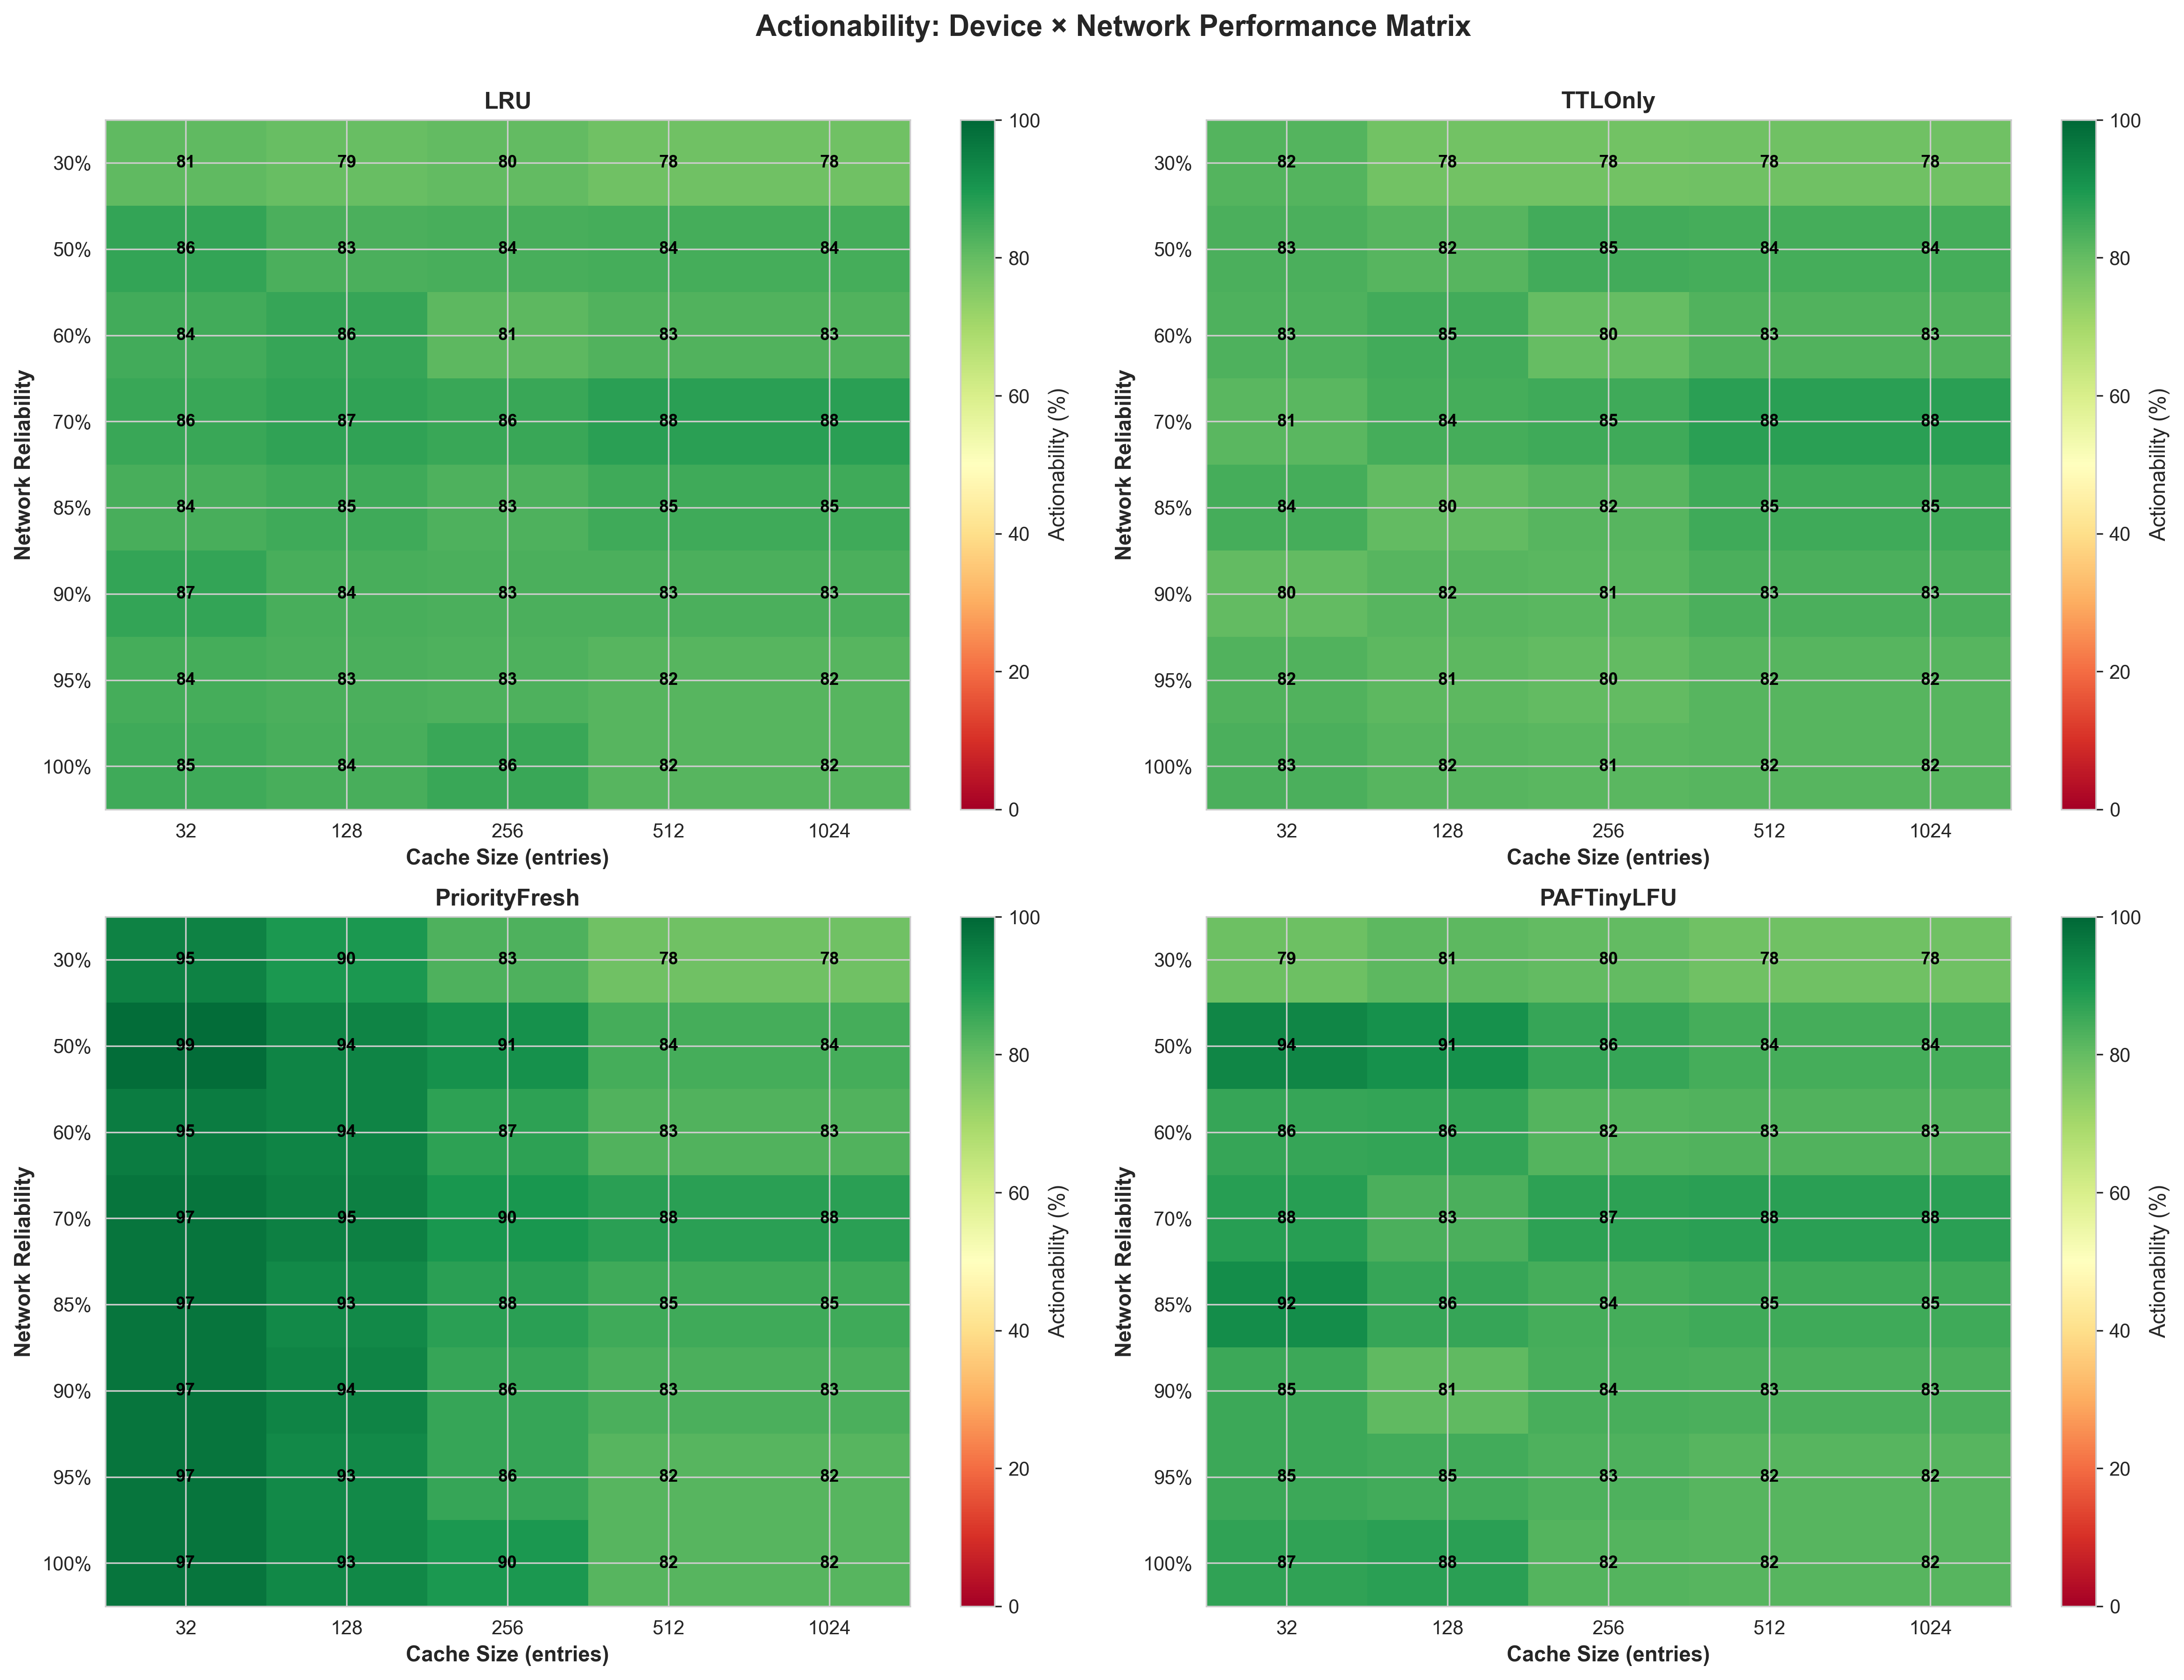
\includegraphics[width=\linewidth]{figures/combined_heatmap_matrix_actionabilityFirstRatio.png}
    \caption{Joint sweep: actionability-first ratio heatmap matrix.}
    \label{fig:combined-heatmap-actionability}
\end{figure}

\begin{figure}[h]
    \centering
    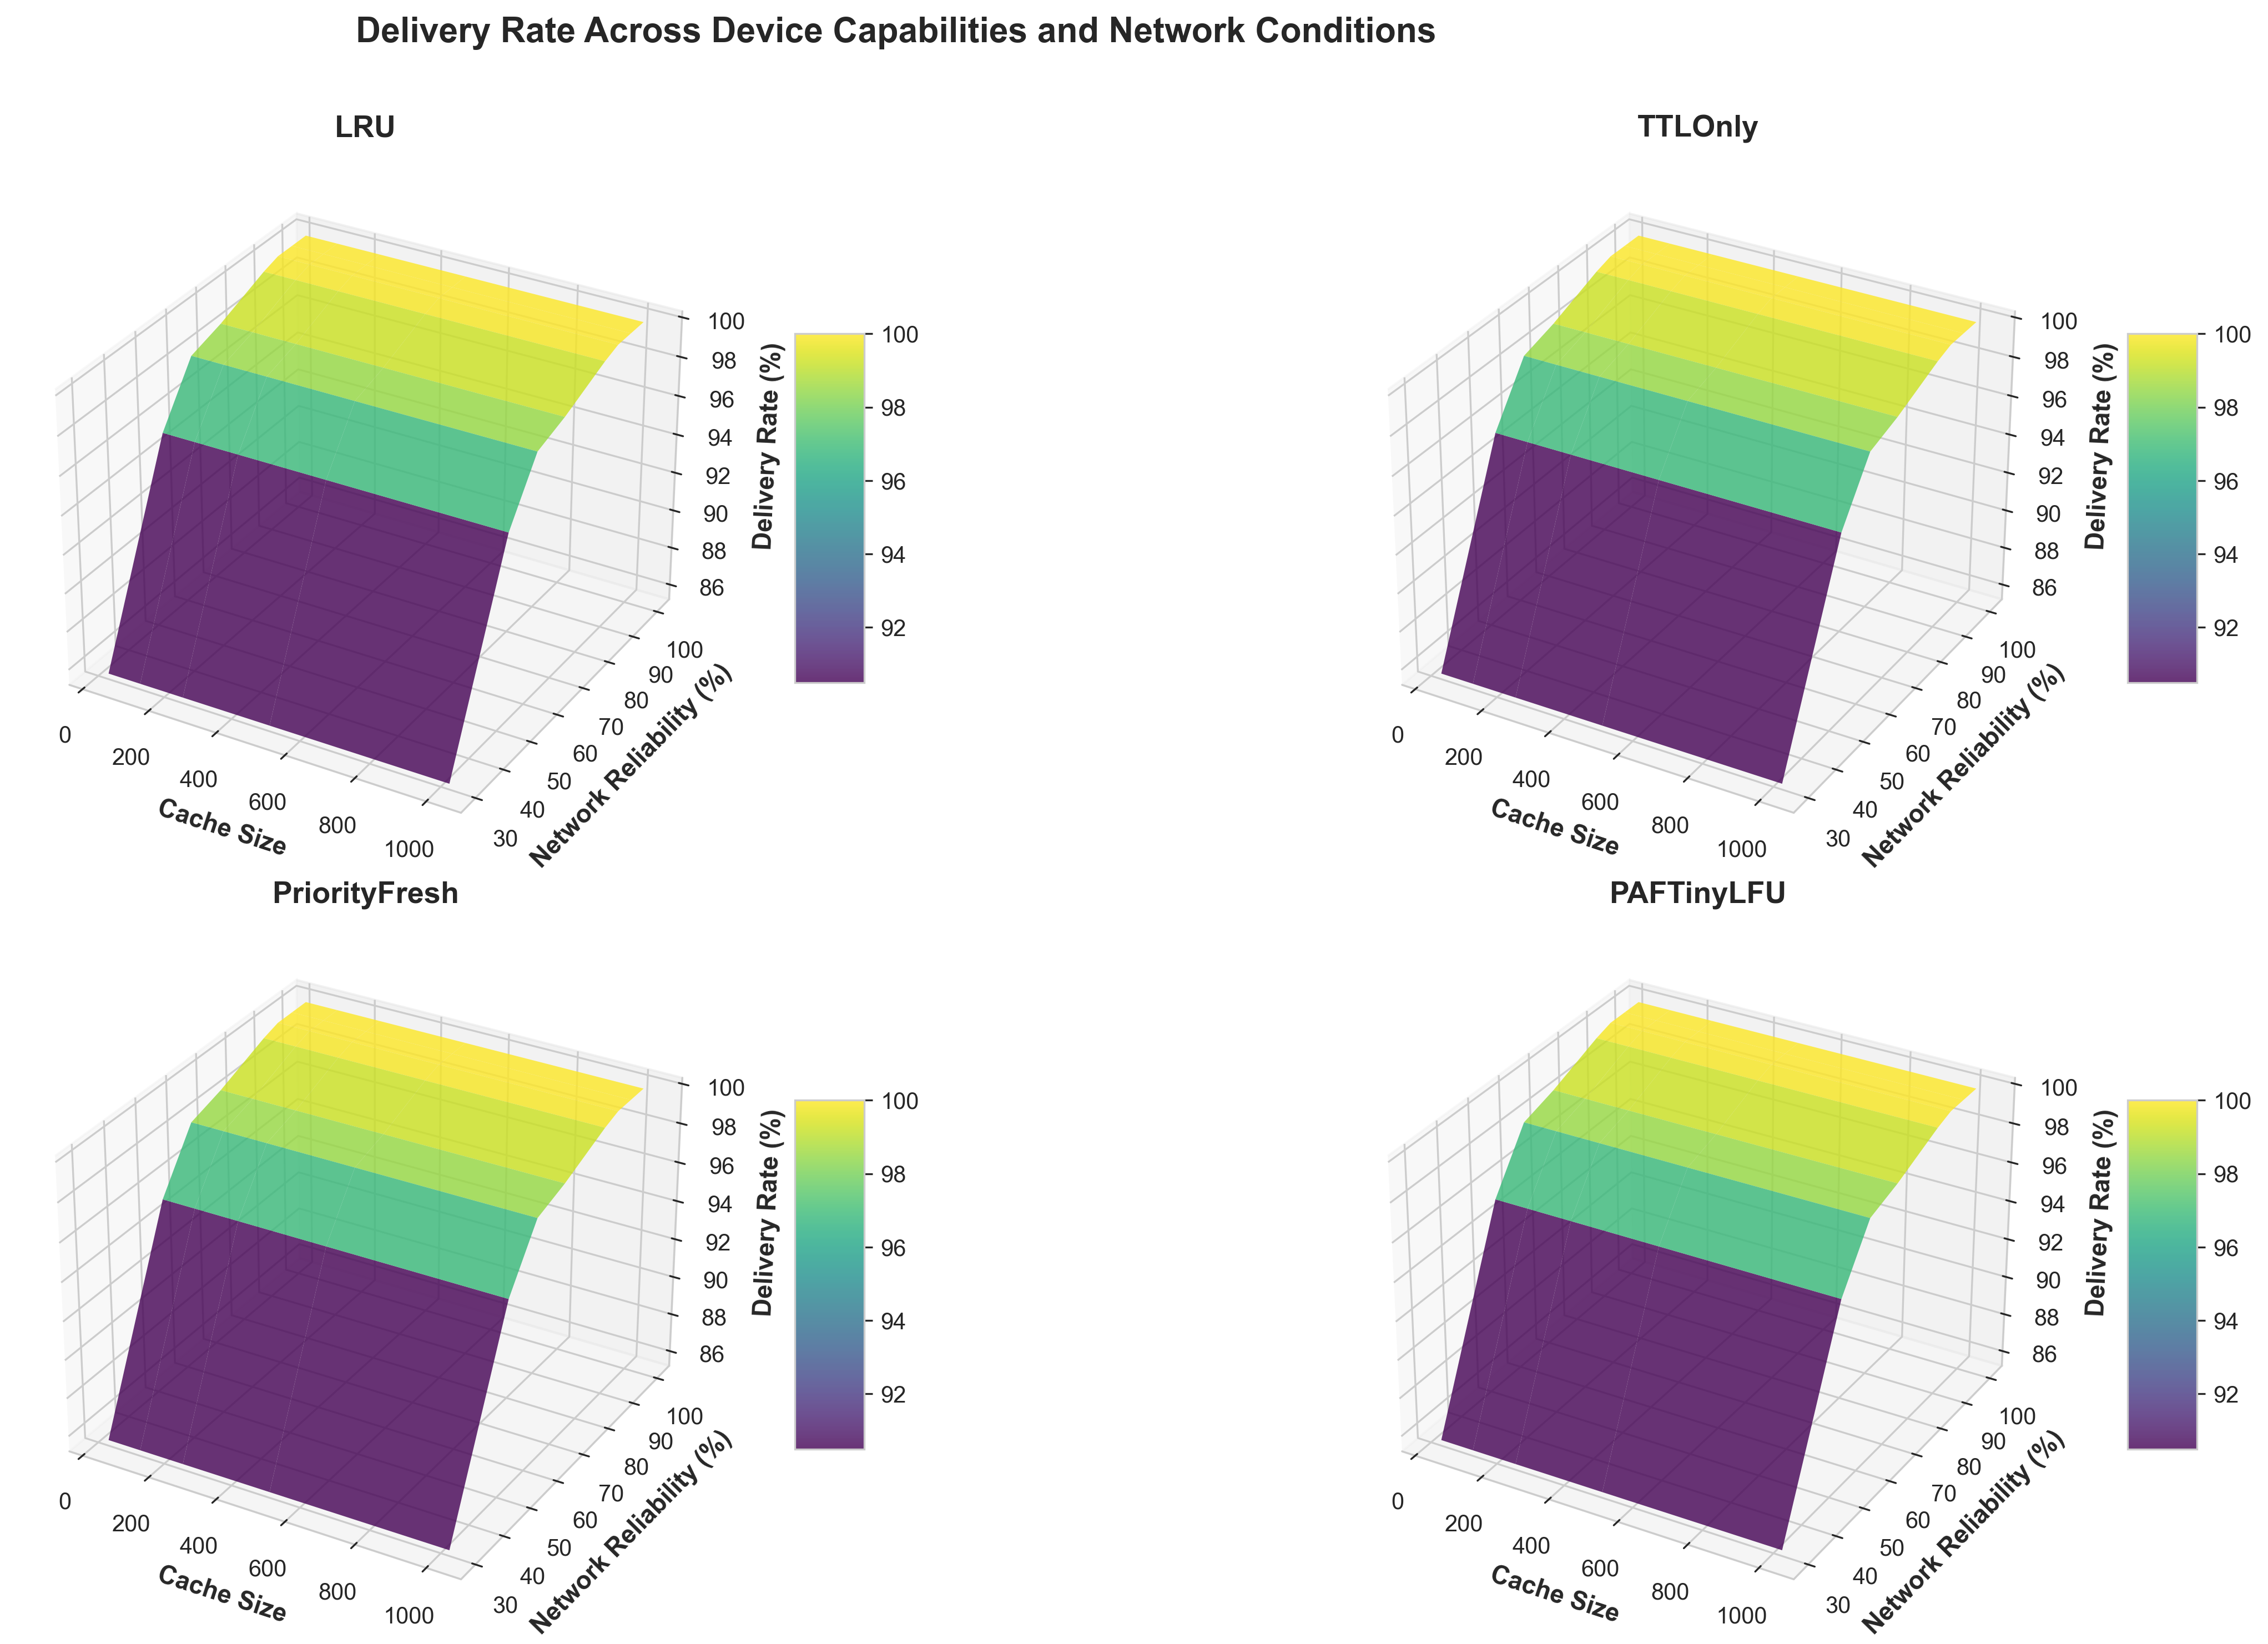
\includegraphics[width=\linewidth]{figures/combined_3d_surface_deliveryRate.png}
    \caption{Joint sweep: delivery rate surface over cache size and network reliability.}
    \label{fig:combined-surface-delivery}
\end{figure}

\begin{figure}[h]
    \centering
    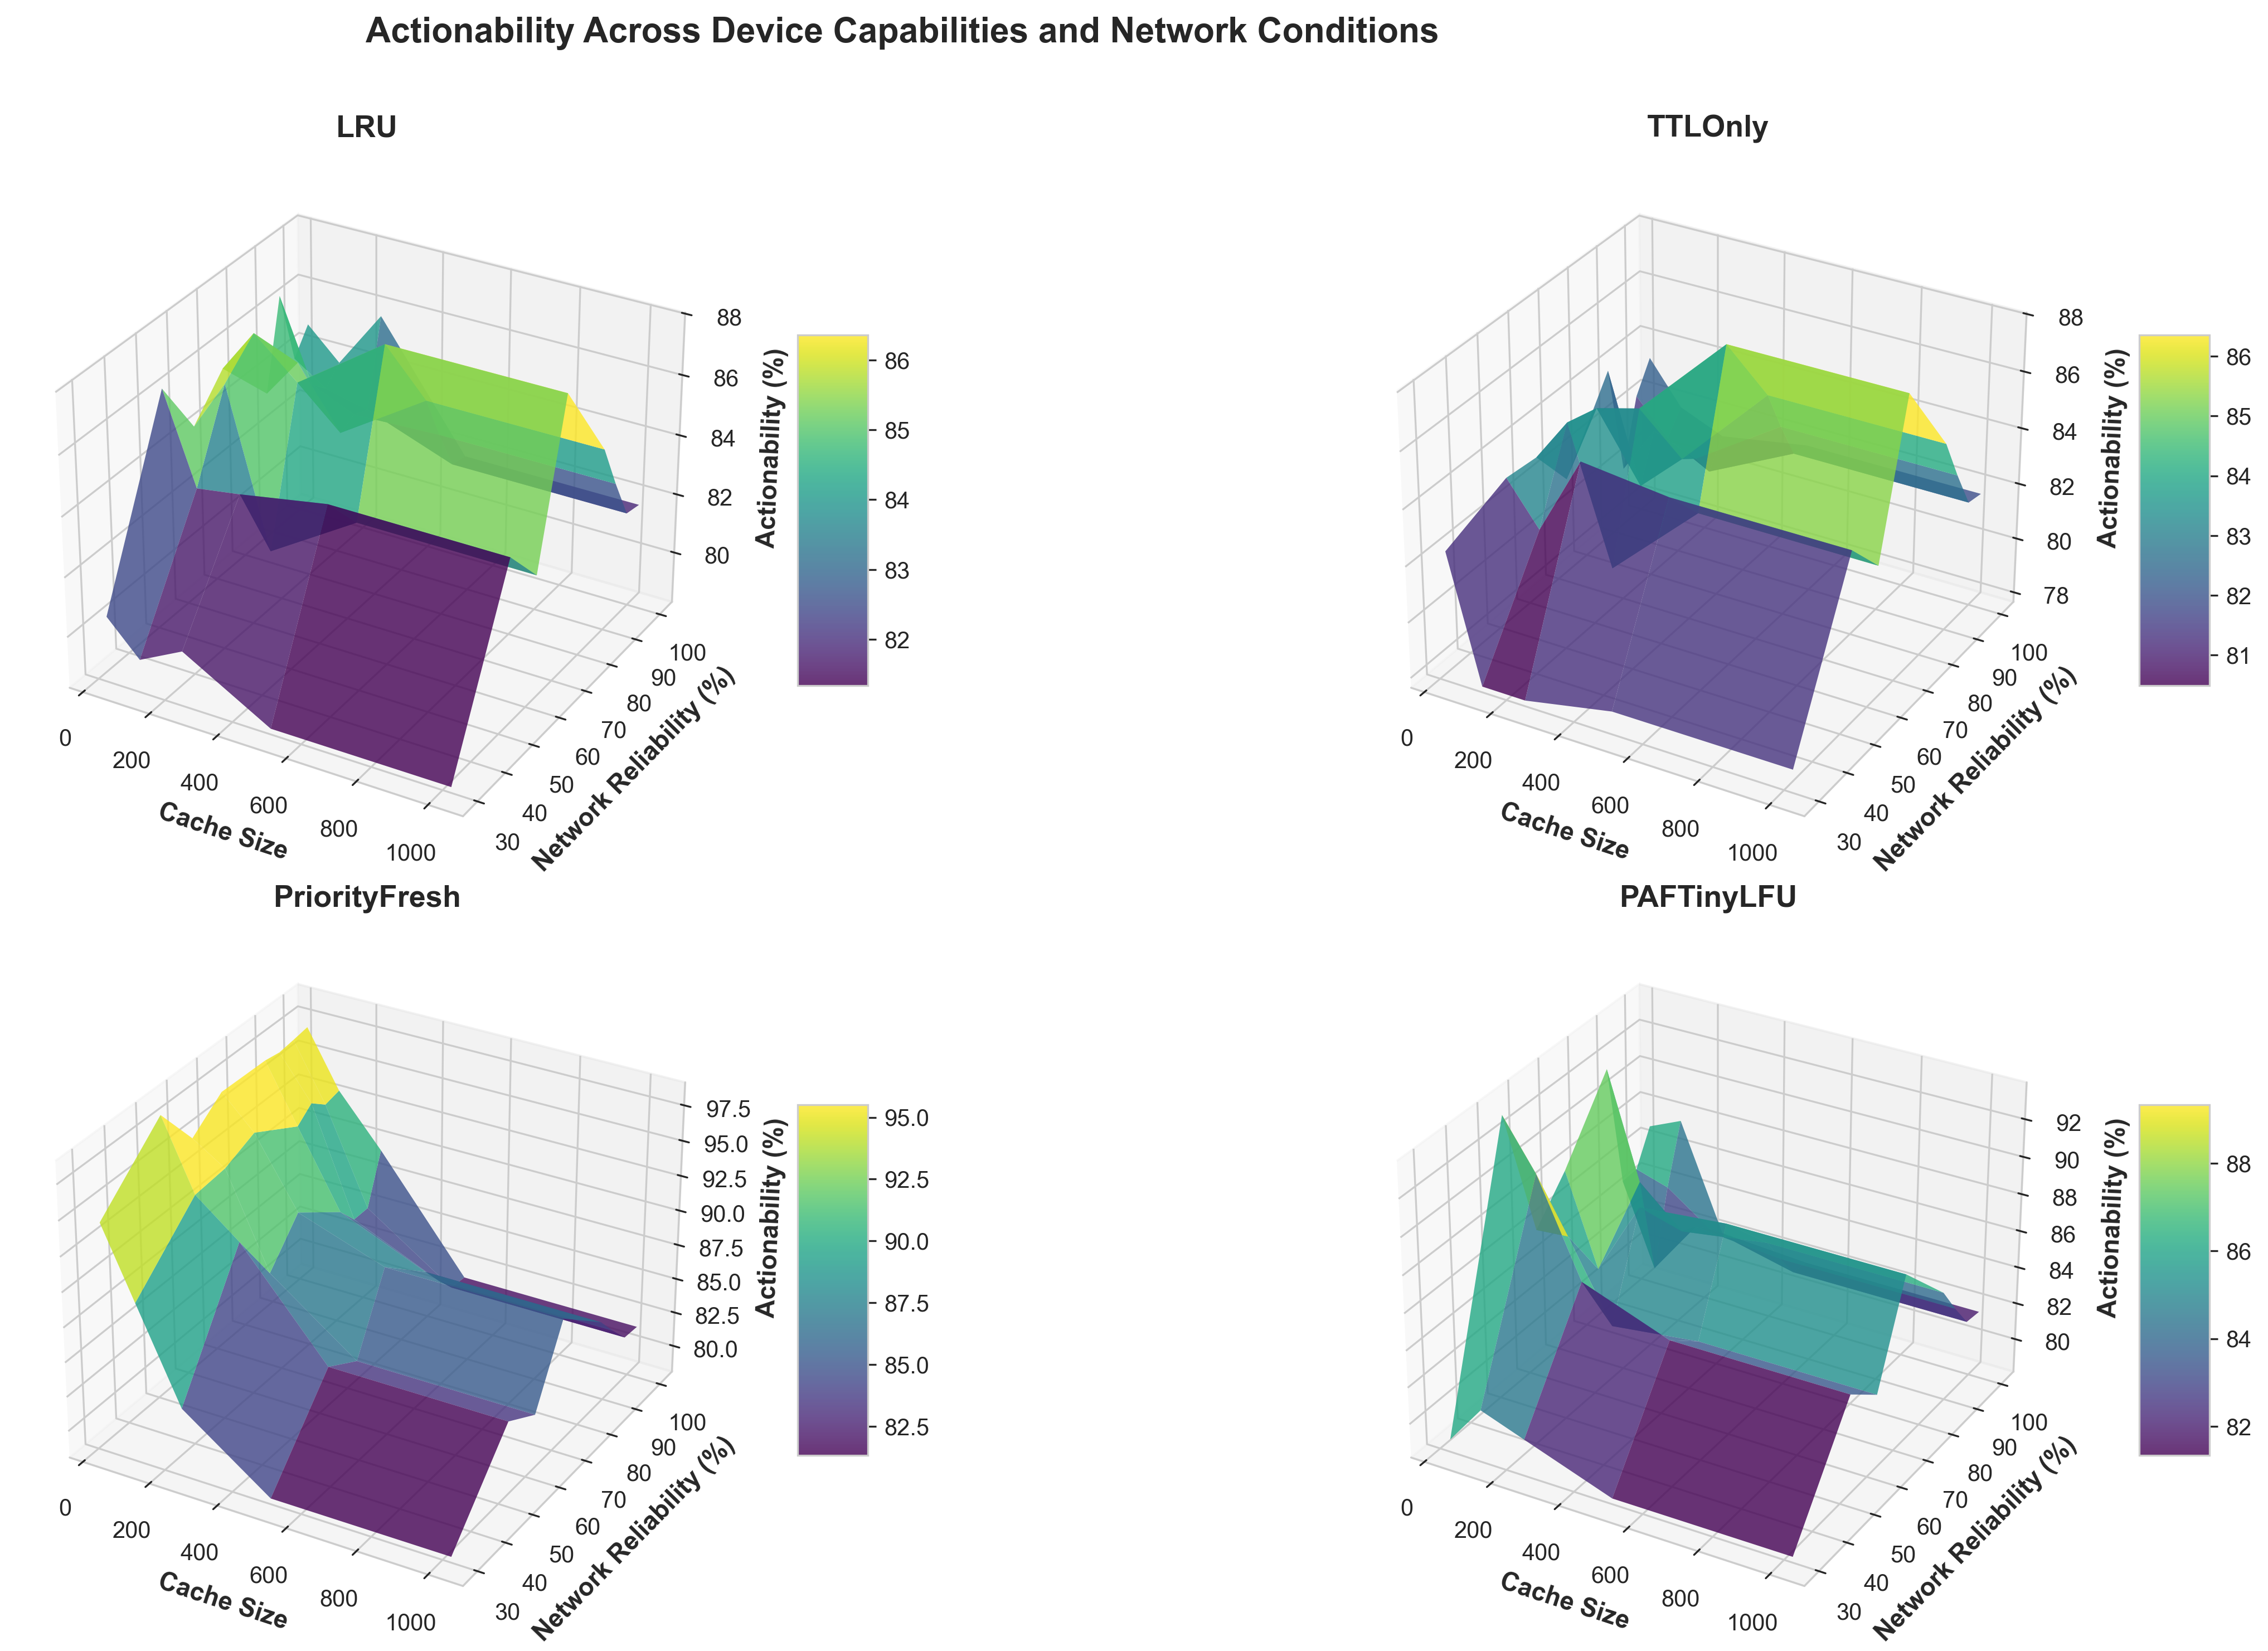
\includegraphics[width=\linewidth]{figures/combined_3d_surface_actionabilityFirstRatio.png}
    \caption{Joint sweep: actionability-first surface over cache size and network reliability.}
    \label{fig:combined-surface-actionability}
\end{figure}

\begin{figure}[h]
    \centering
    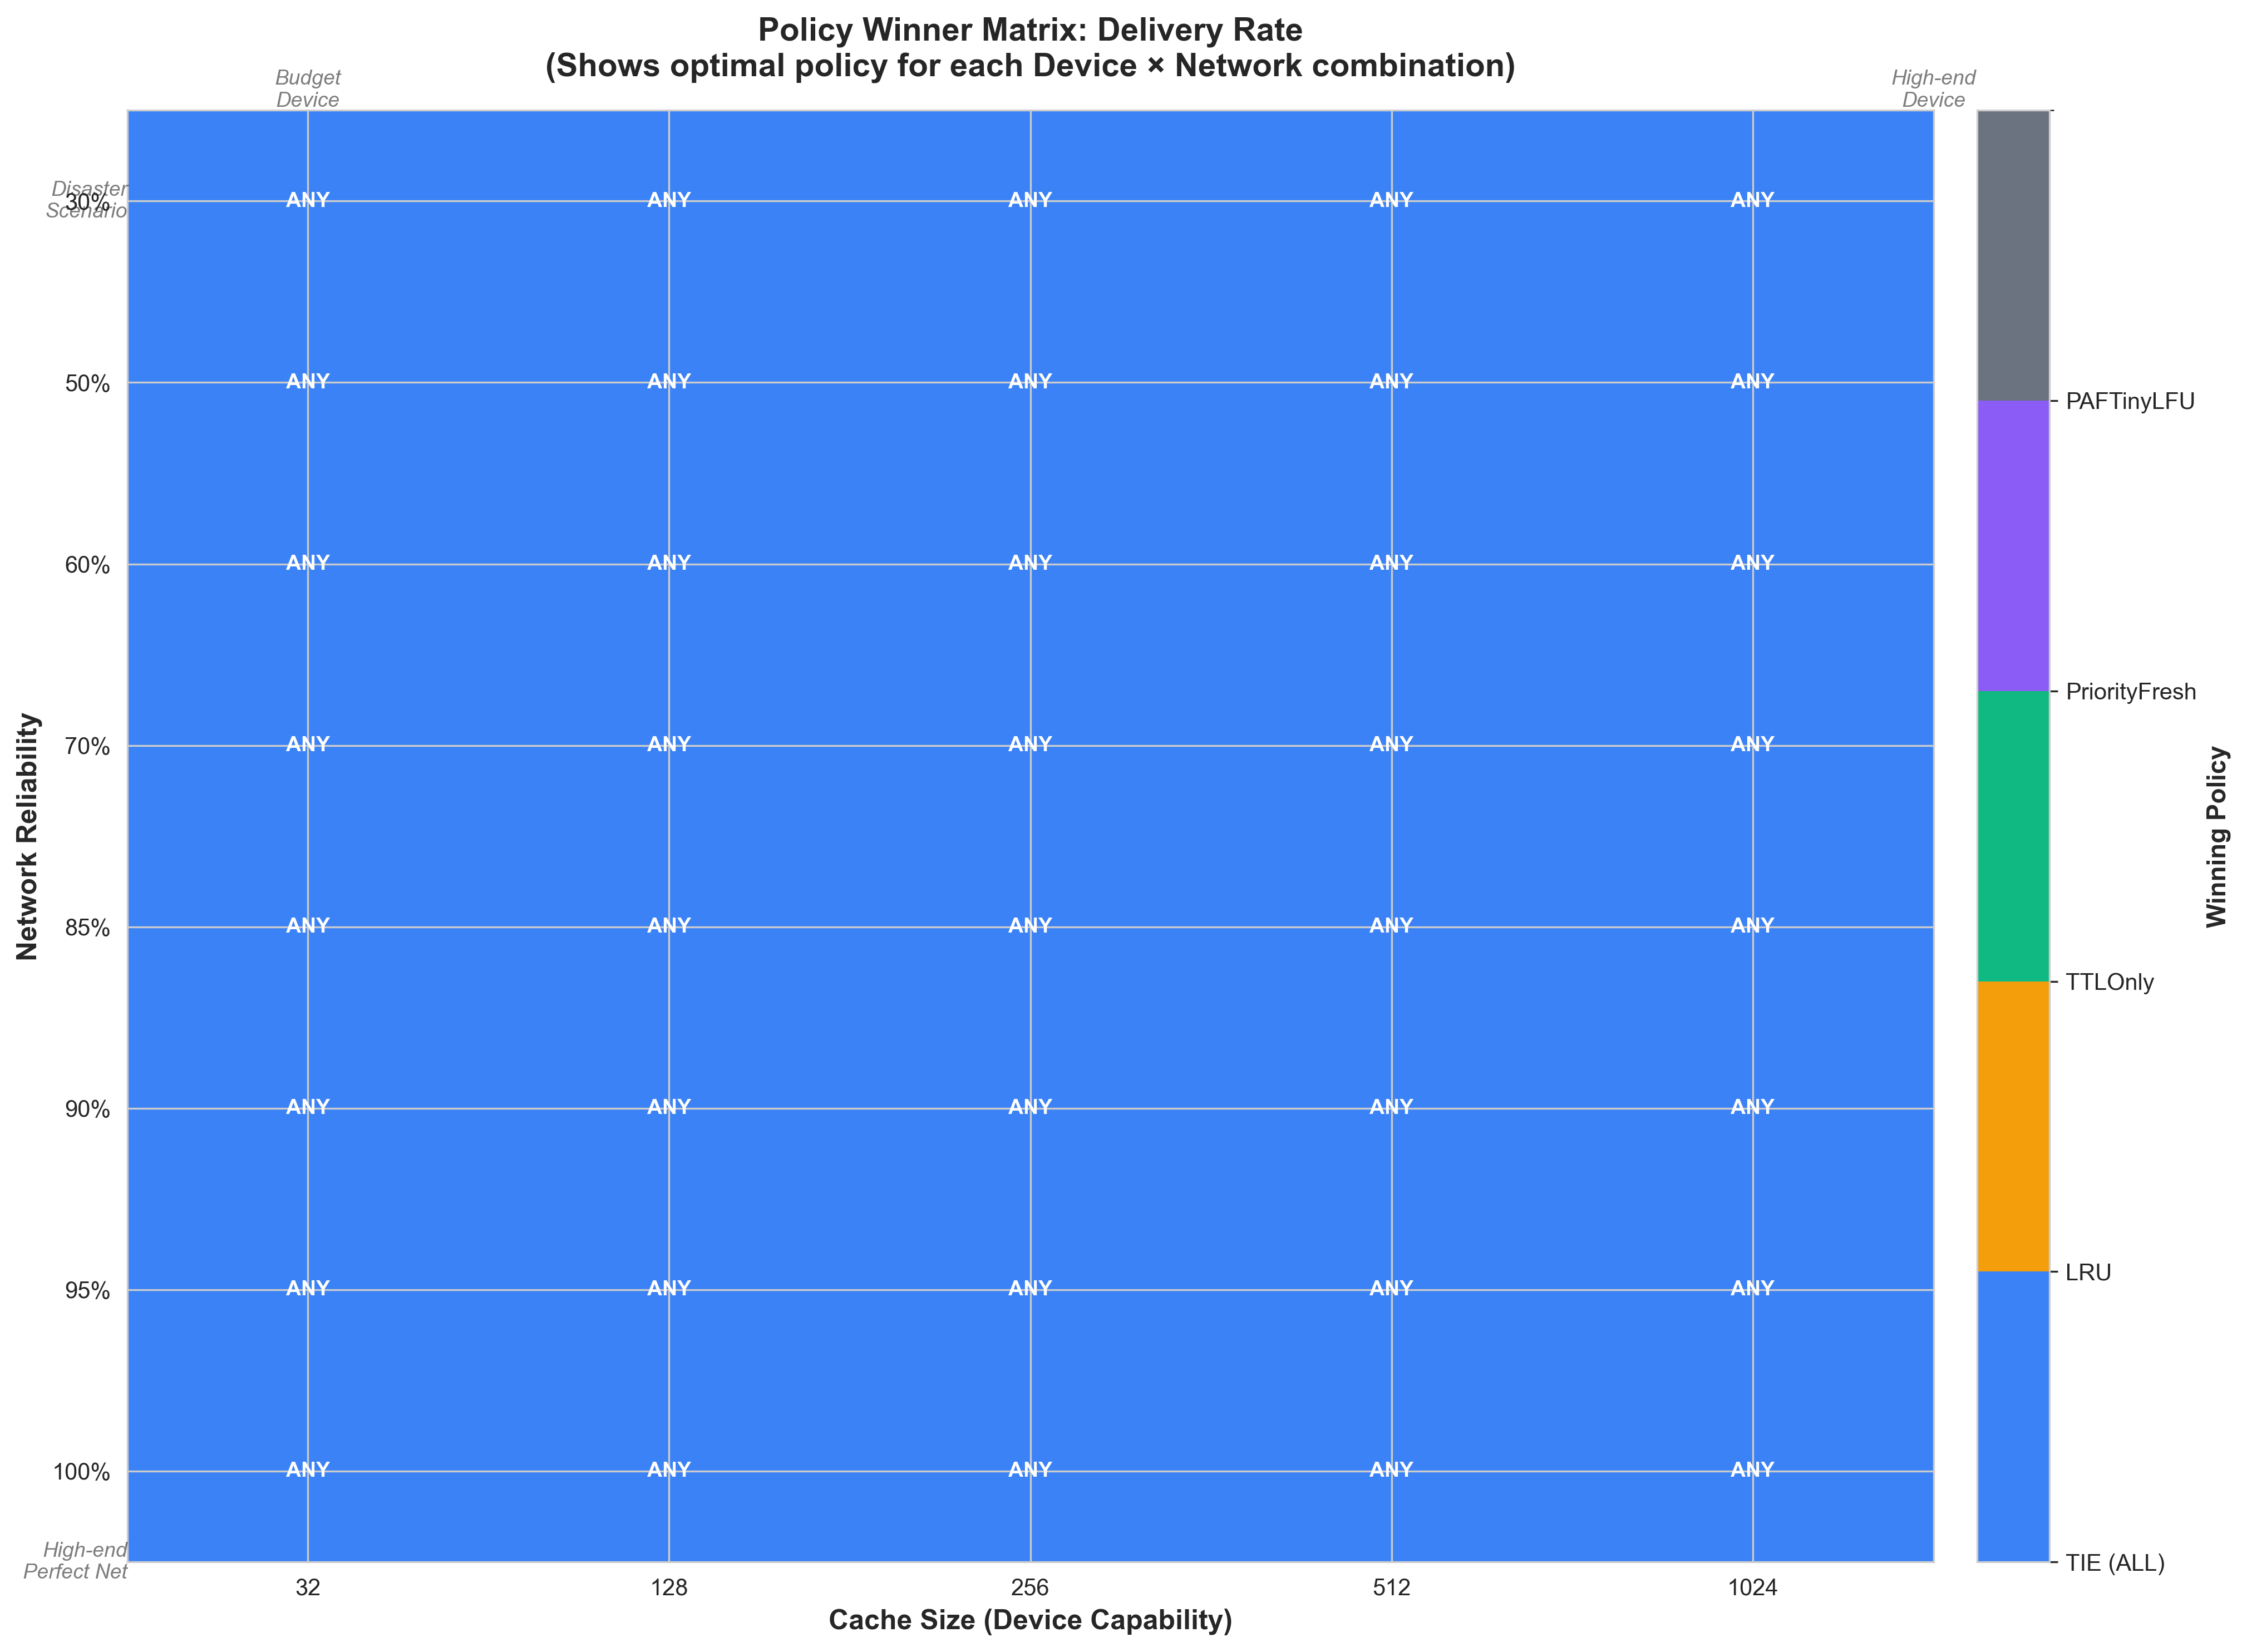
\includegraphics[width=\linewidth]{figures/combined_winner_cube_deliveryRate.png}
    \caption{Joint sweep: winner cube (delivery rate).}
    \label{fig:combined-winner-cube-delivery}
\end{figure}

\begin{figure}[h]
    \centering
    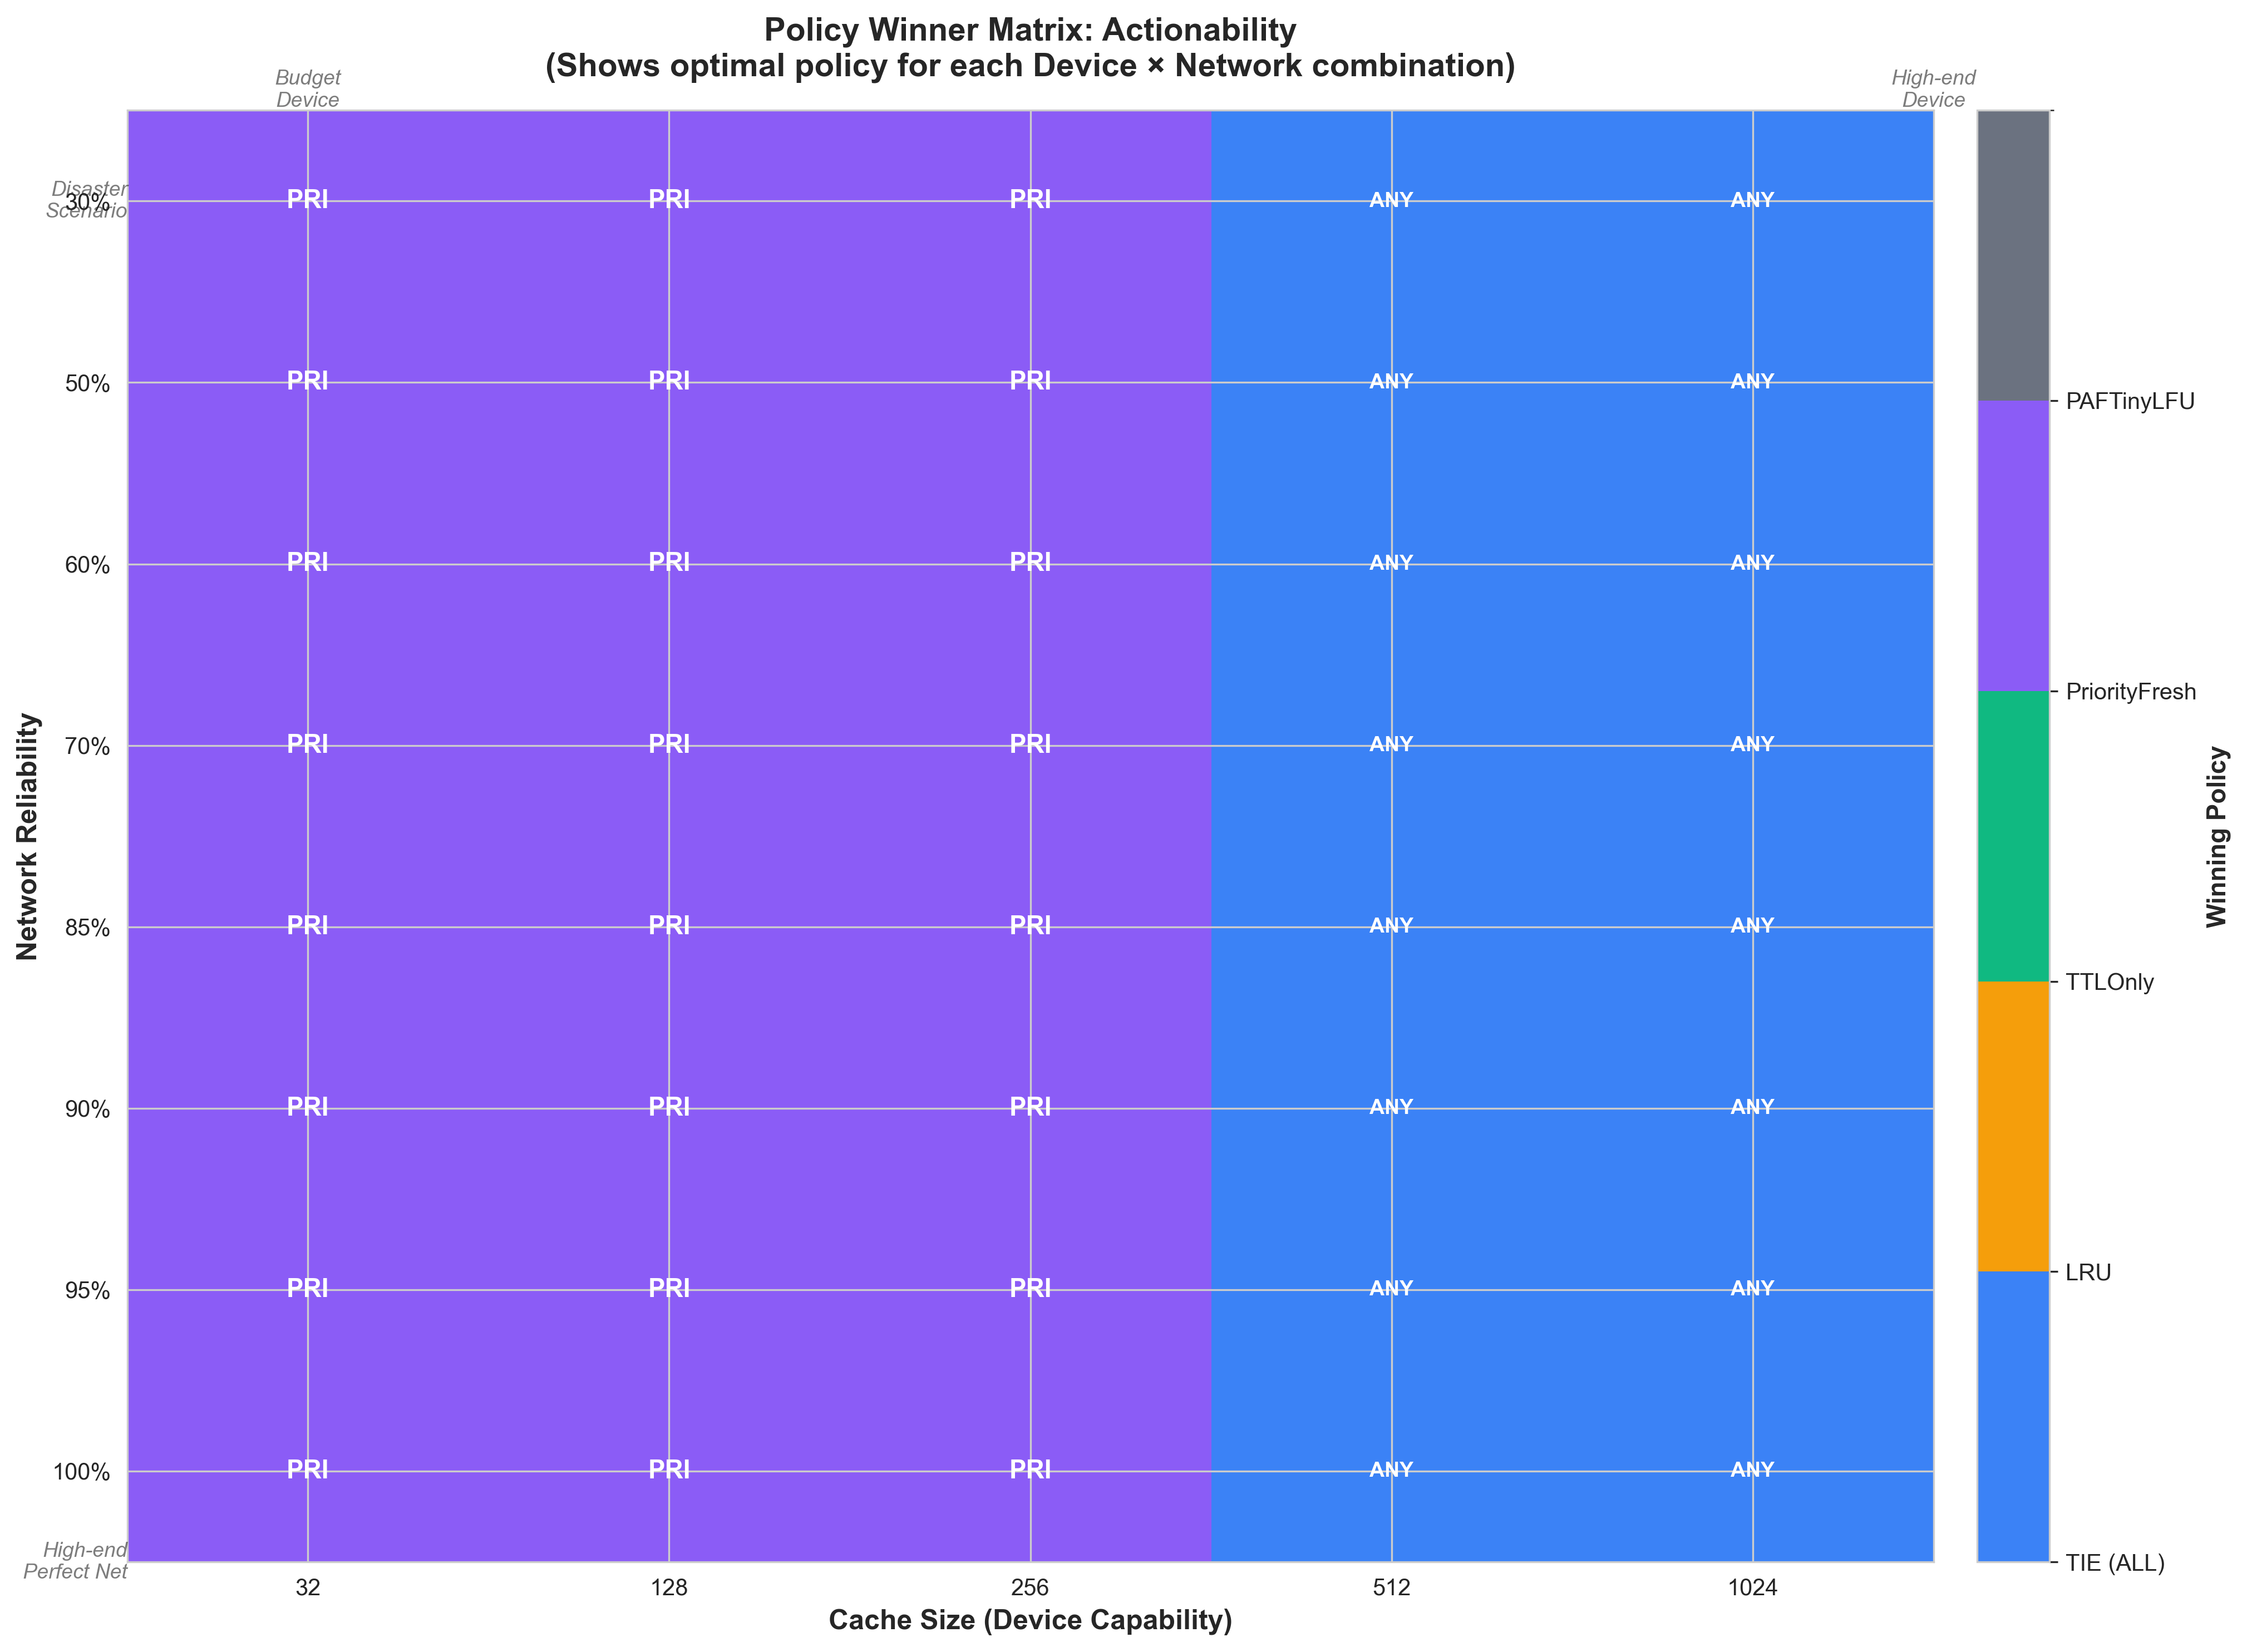
\includegraphics[width=\linewidth]{figures/combined_winner_cube_actionabilityFirstRatio.png}
    \caption{Joint sweep: winner cube (actionability-first).}
    \label{fig:combined-winner-cube-actionability}
\end{figure}

\begin{figure}[h]
    \centering
    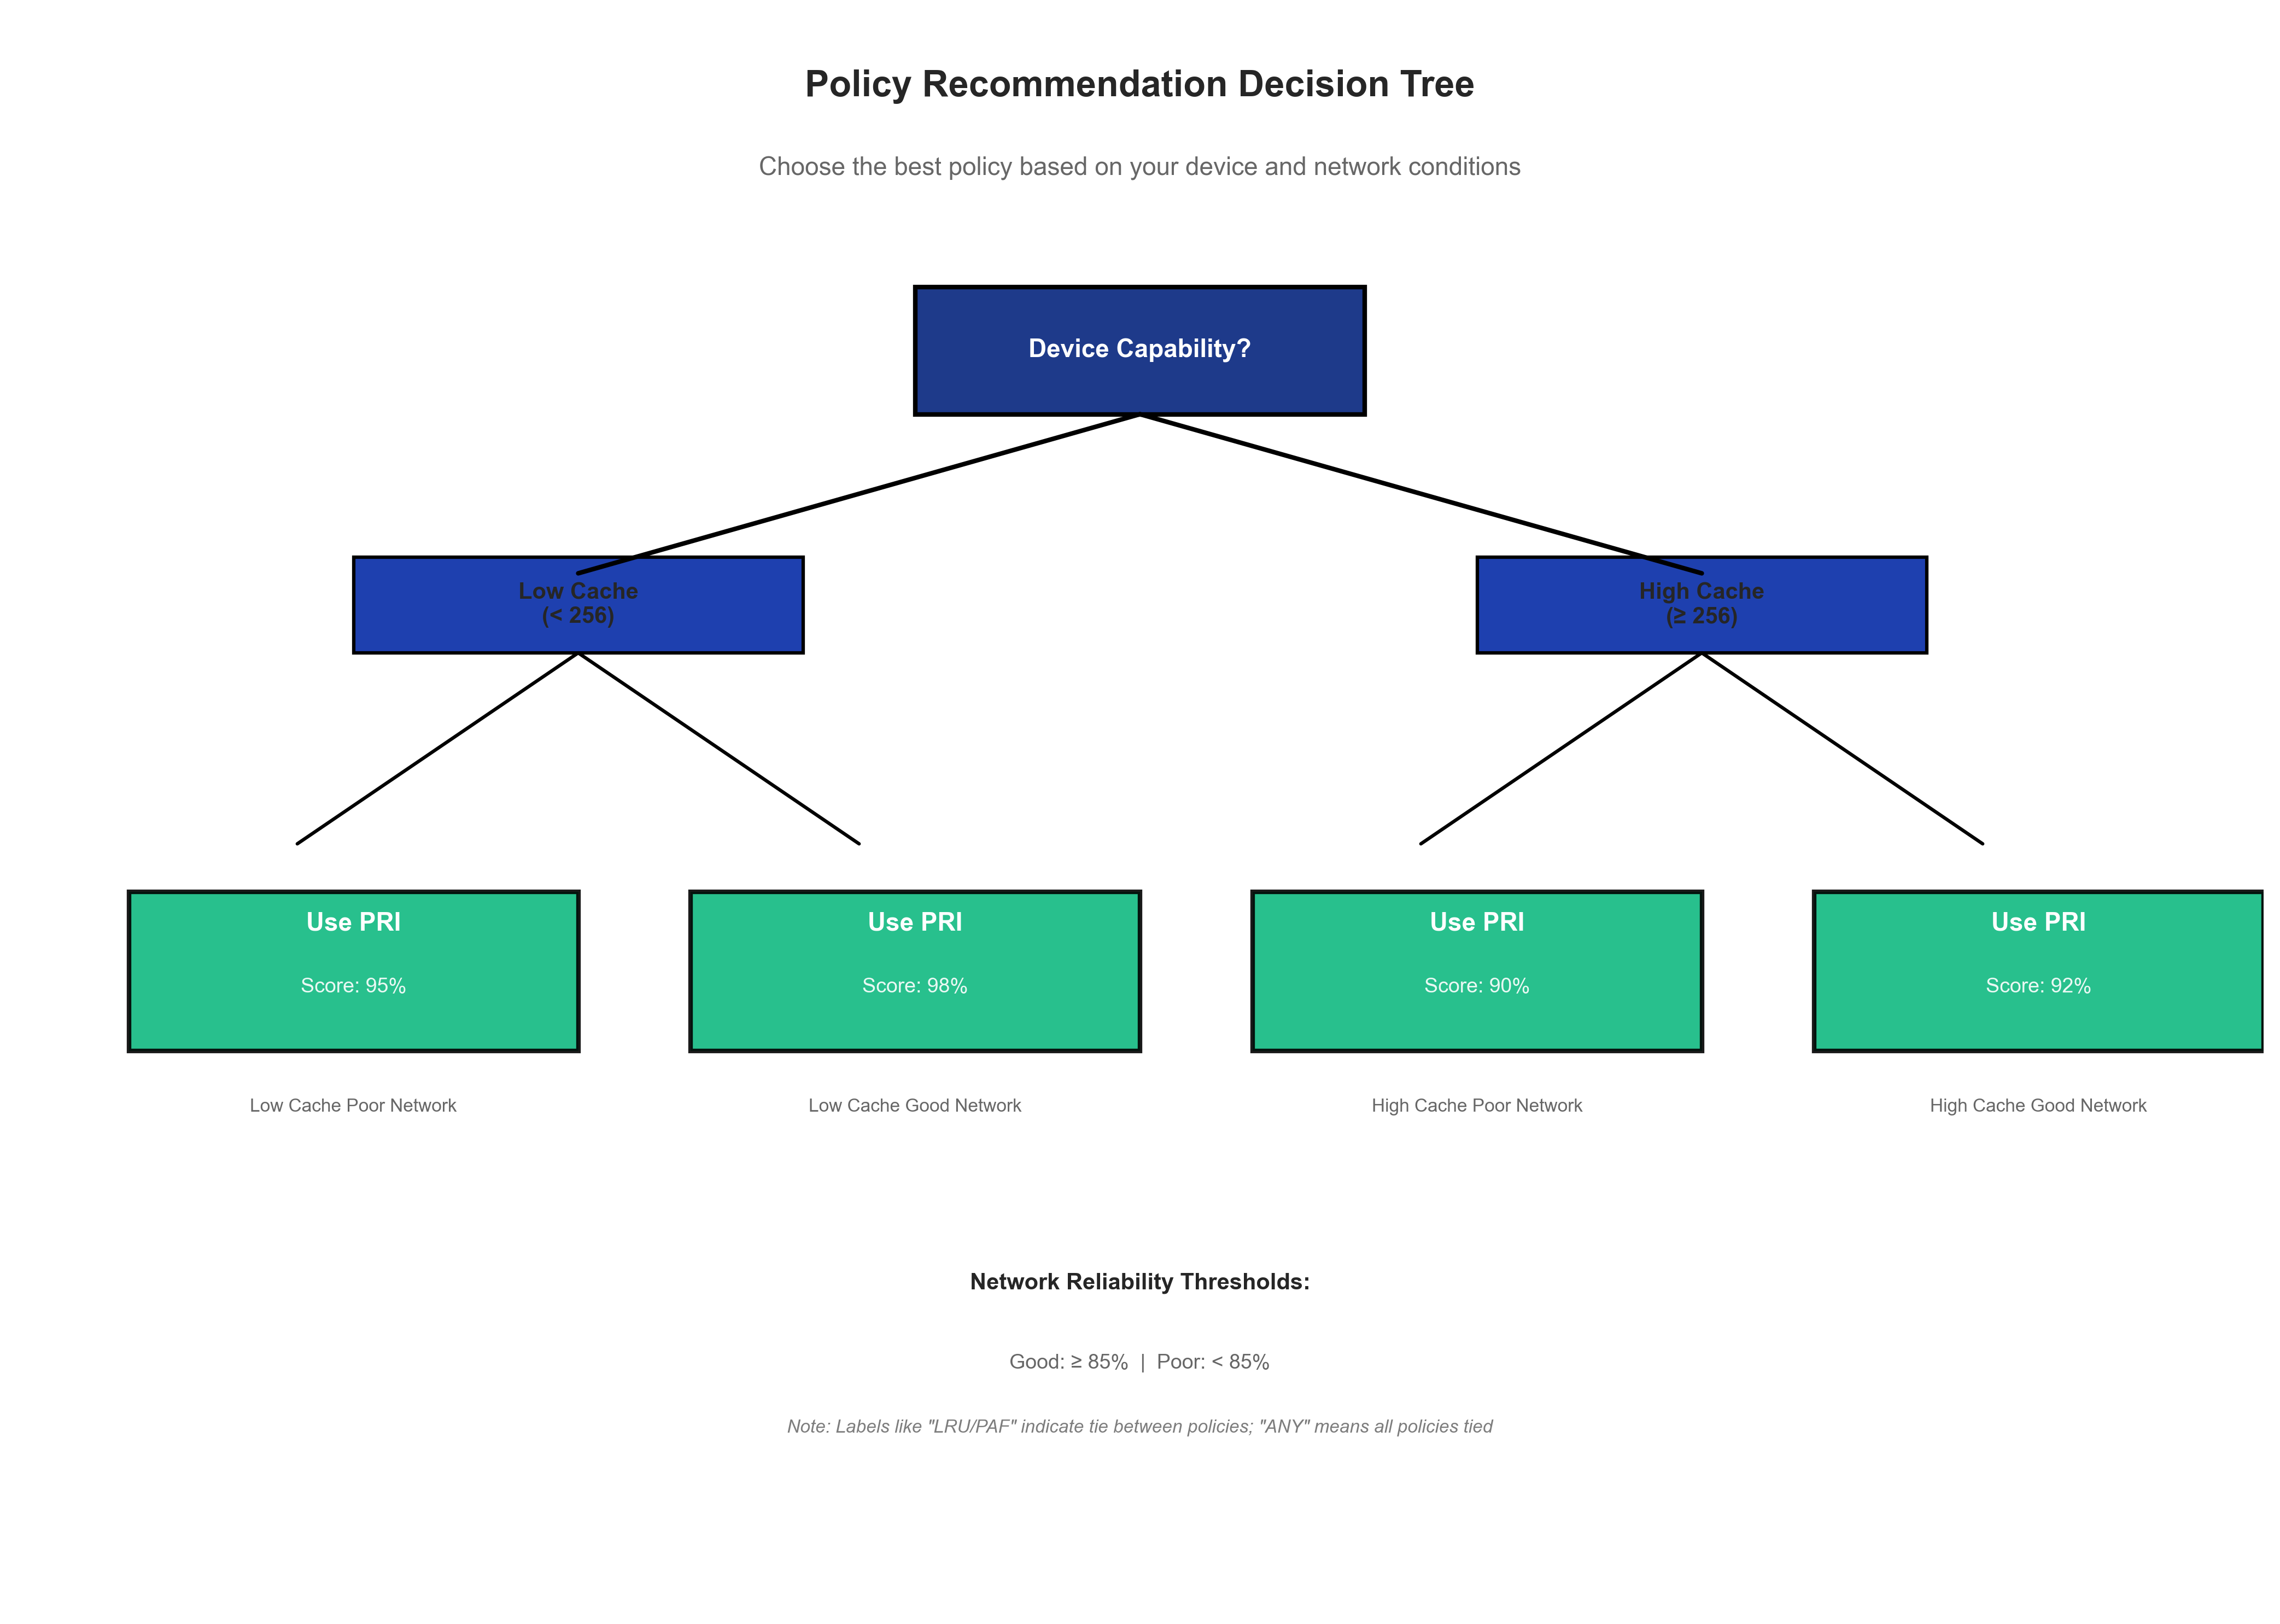
\includegraphics[width=\linewidth]{figures/combined_recommendation_tree.png}
    \caption{Joint sweep: parameter recommendation tree (policy selection guide).}
    \label{fig:combined-reco-tree}
\end{figure}

\subsubsection{Optional timeline views}
\begin{figure}[h]
    \centering
    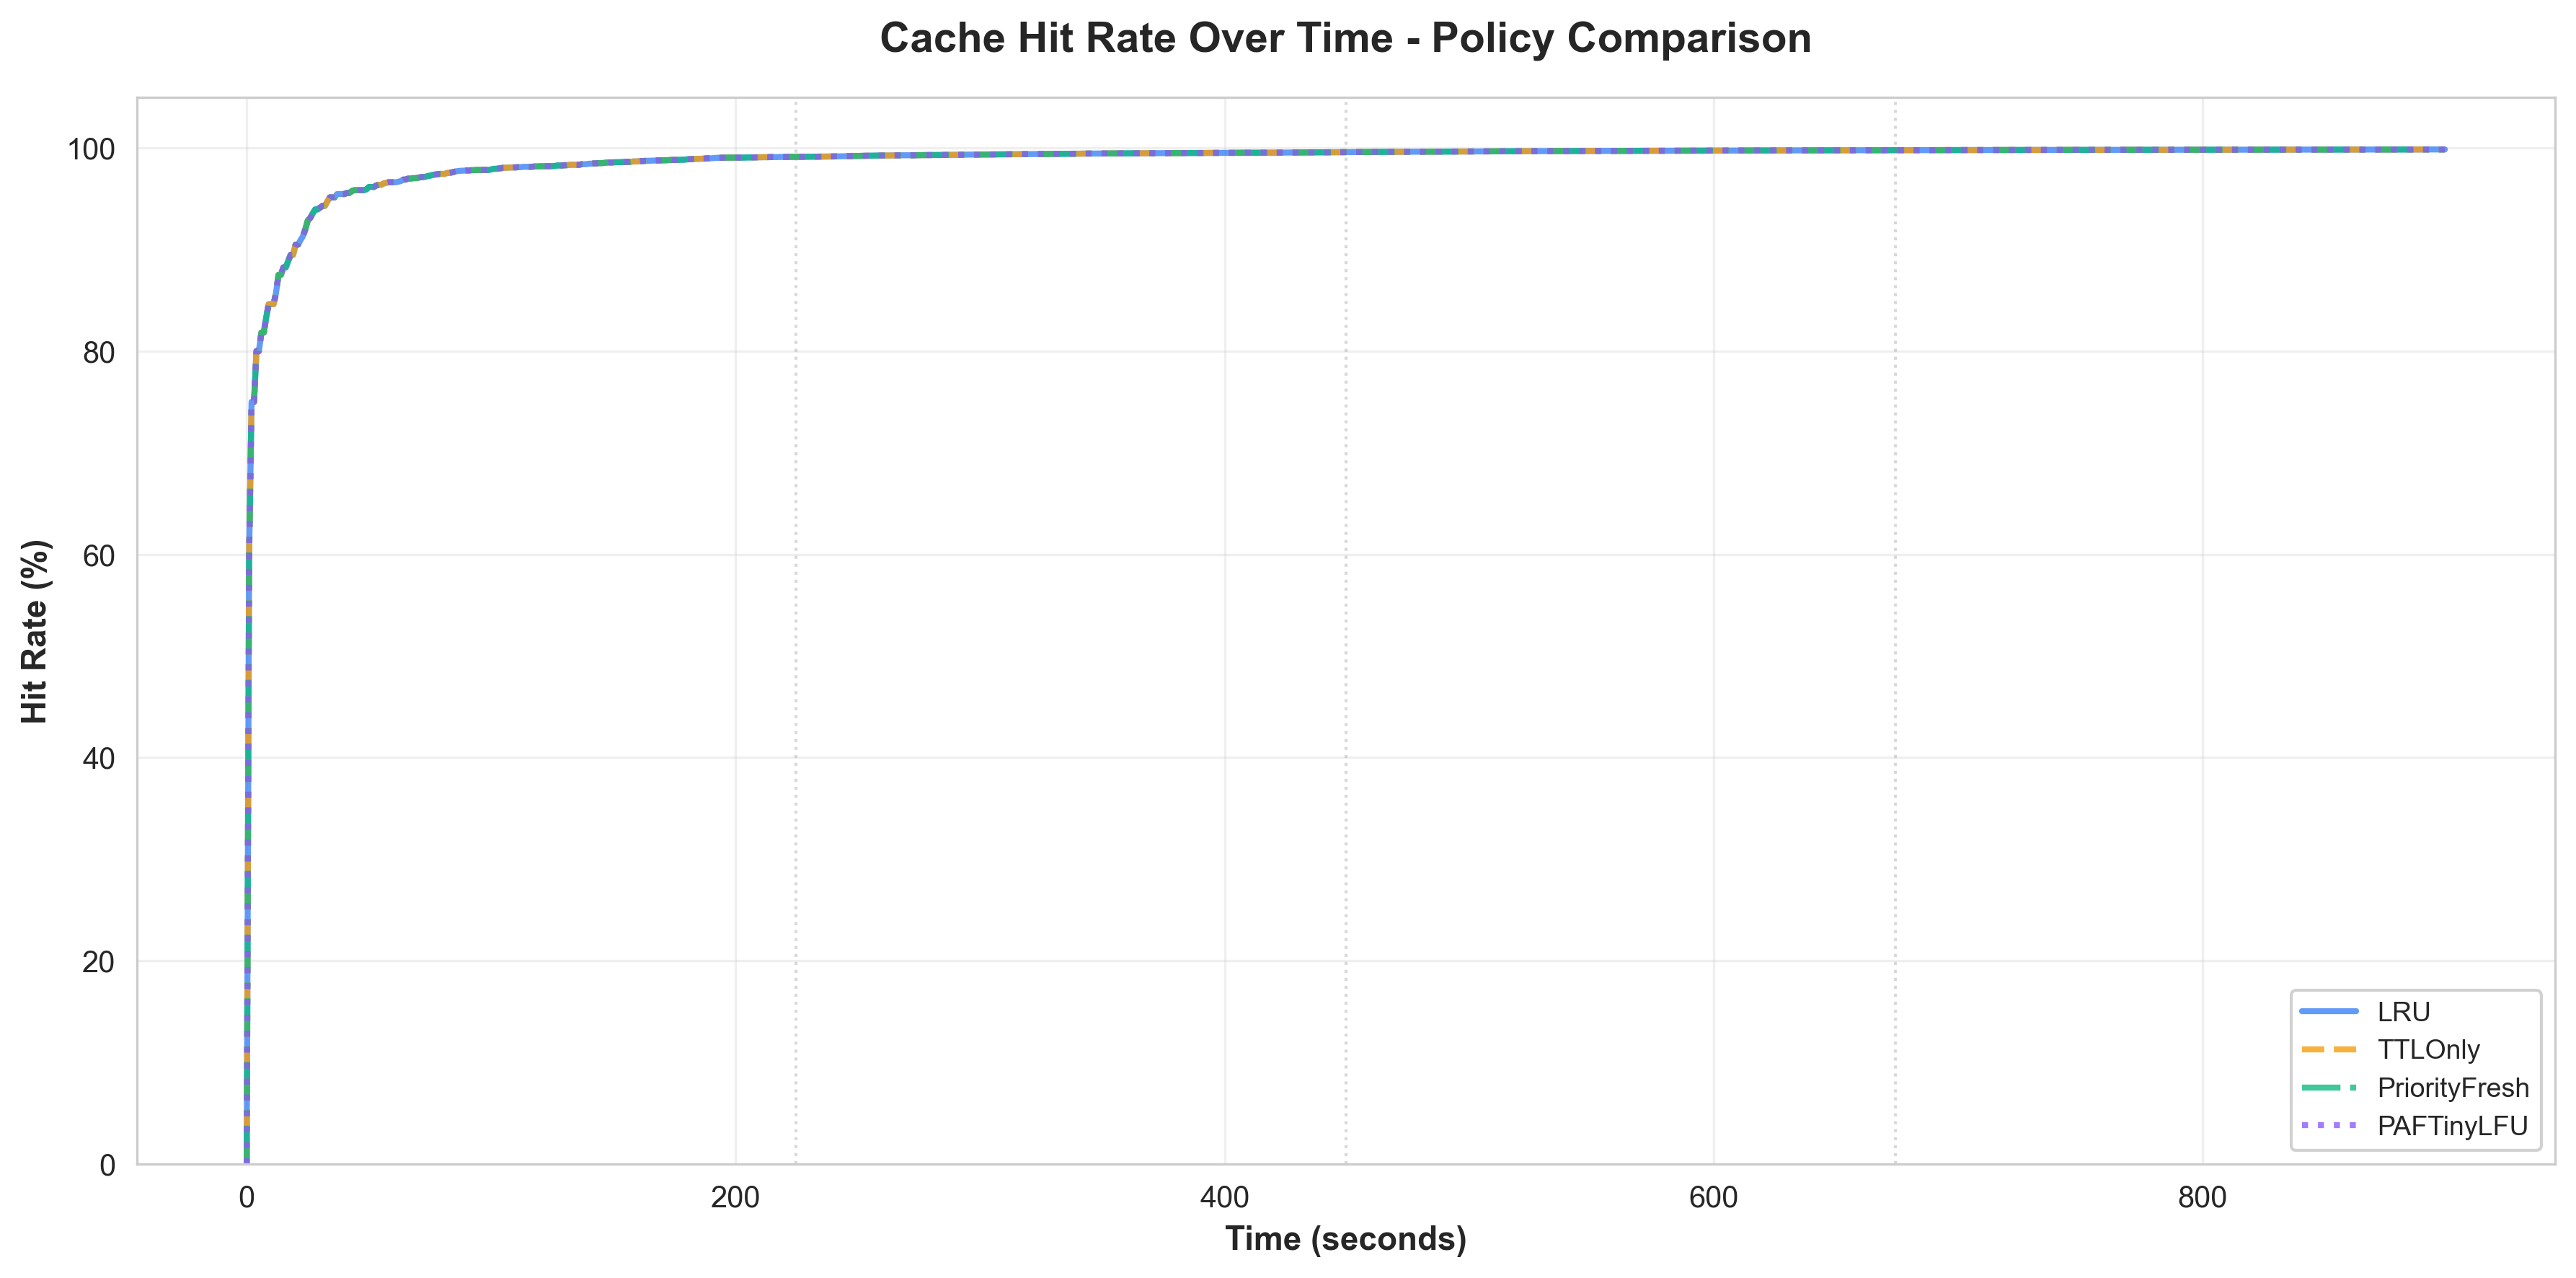
\includegraphics[width=\linewidth]{figures/timeline_hit_rate_timeline.png}
    \caption{Per-run hit rate over time under the baseline configuration.}
    \label{fig:timeline-hitrate}
\end{figure}

\begin{figure}[h]
    \centering
    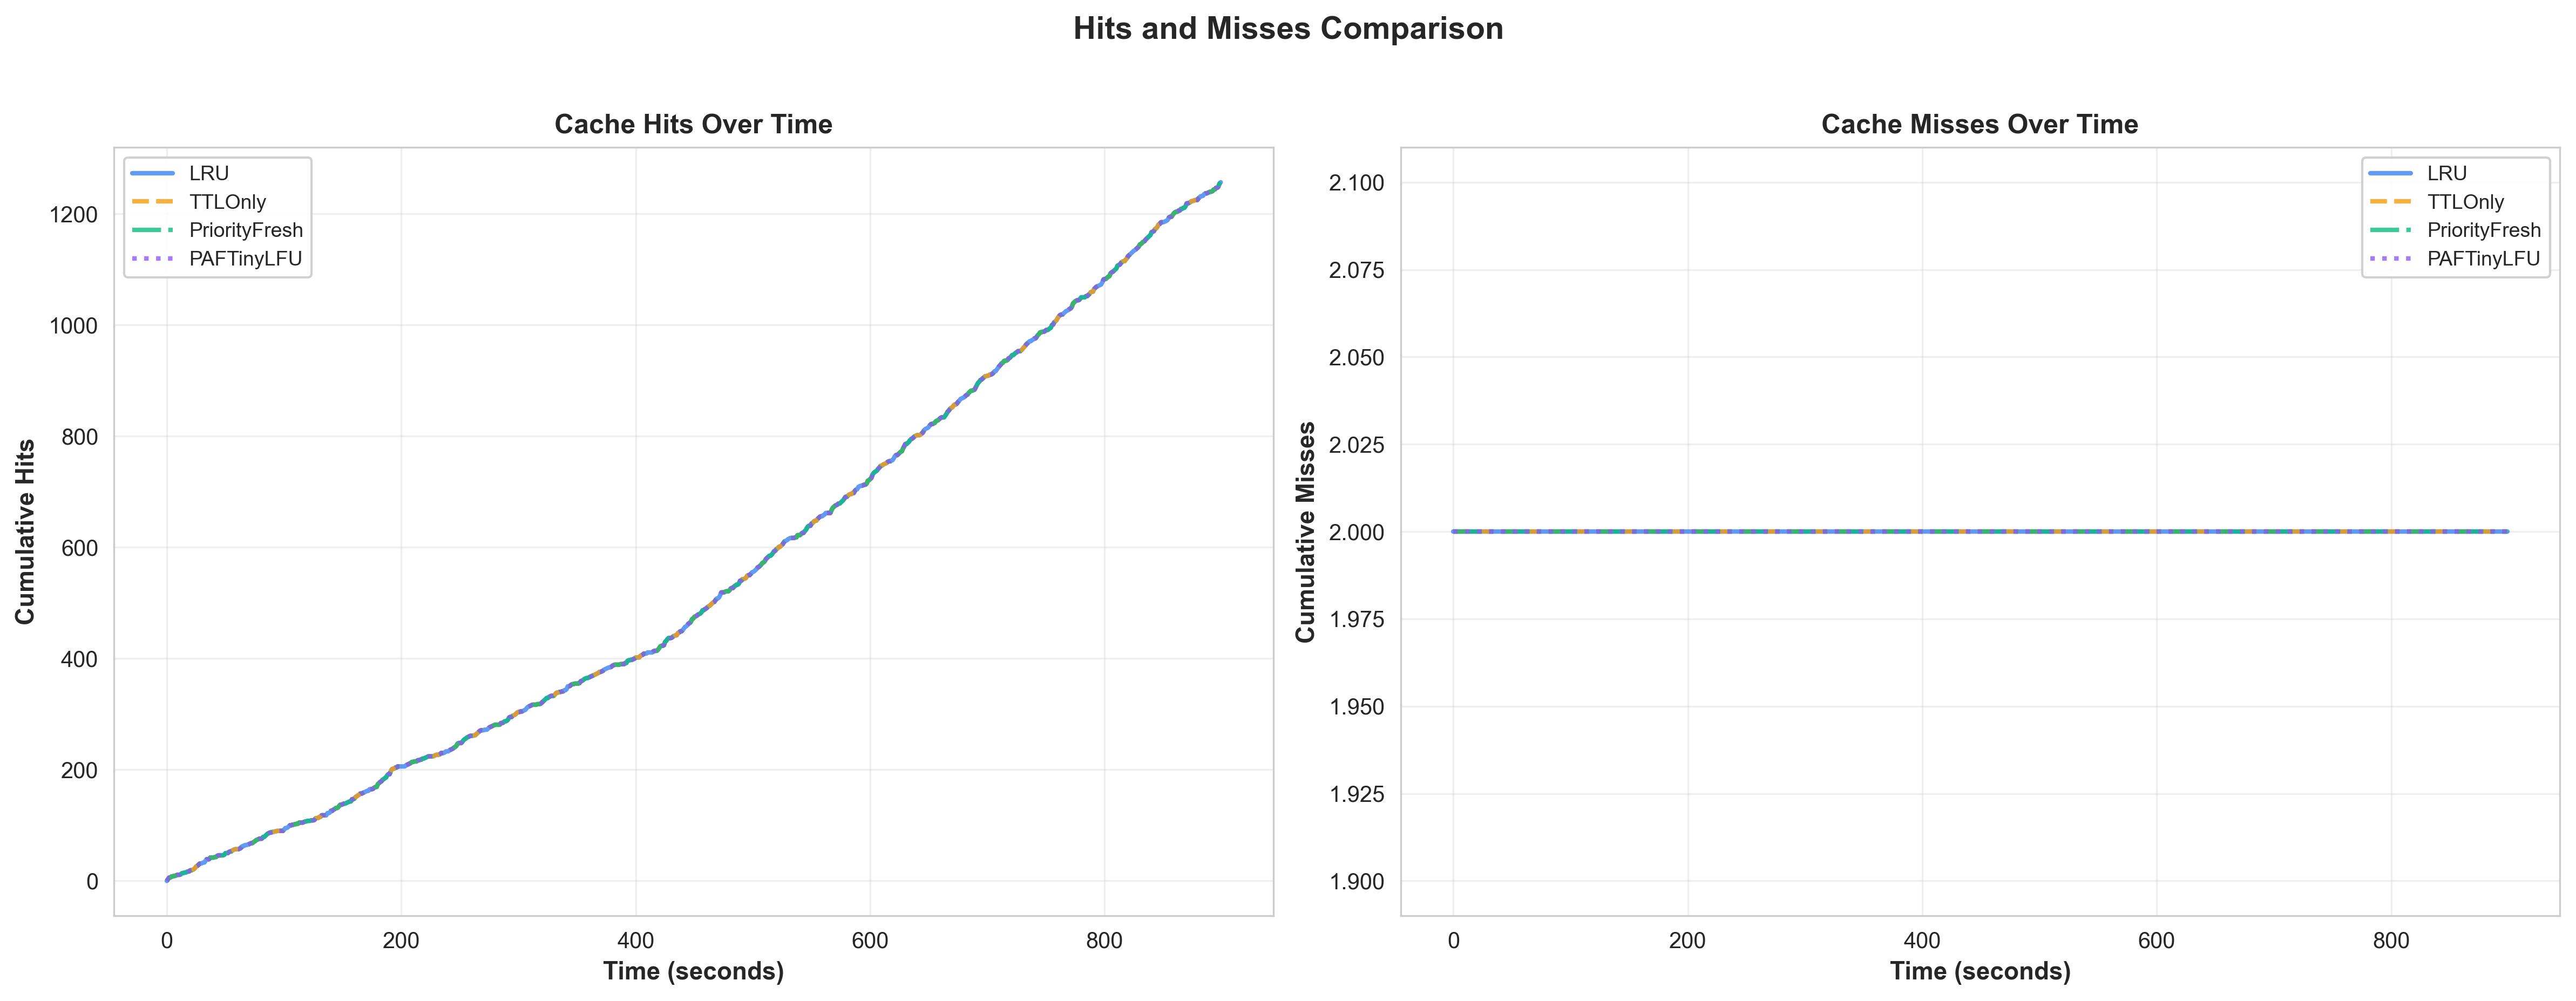
\includegraphics[width=\linewidth]{figures/timeline_hits_misses_timeline.png}
    \caption{Cumulative hits and misses timeline under the baseline configuration.}
    \label{fig:timeline-hits-misses}
\end{figure}

\begin{figure}[h]
    \centering
    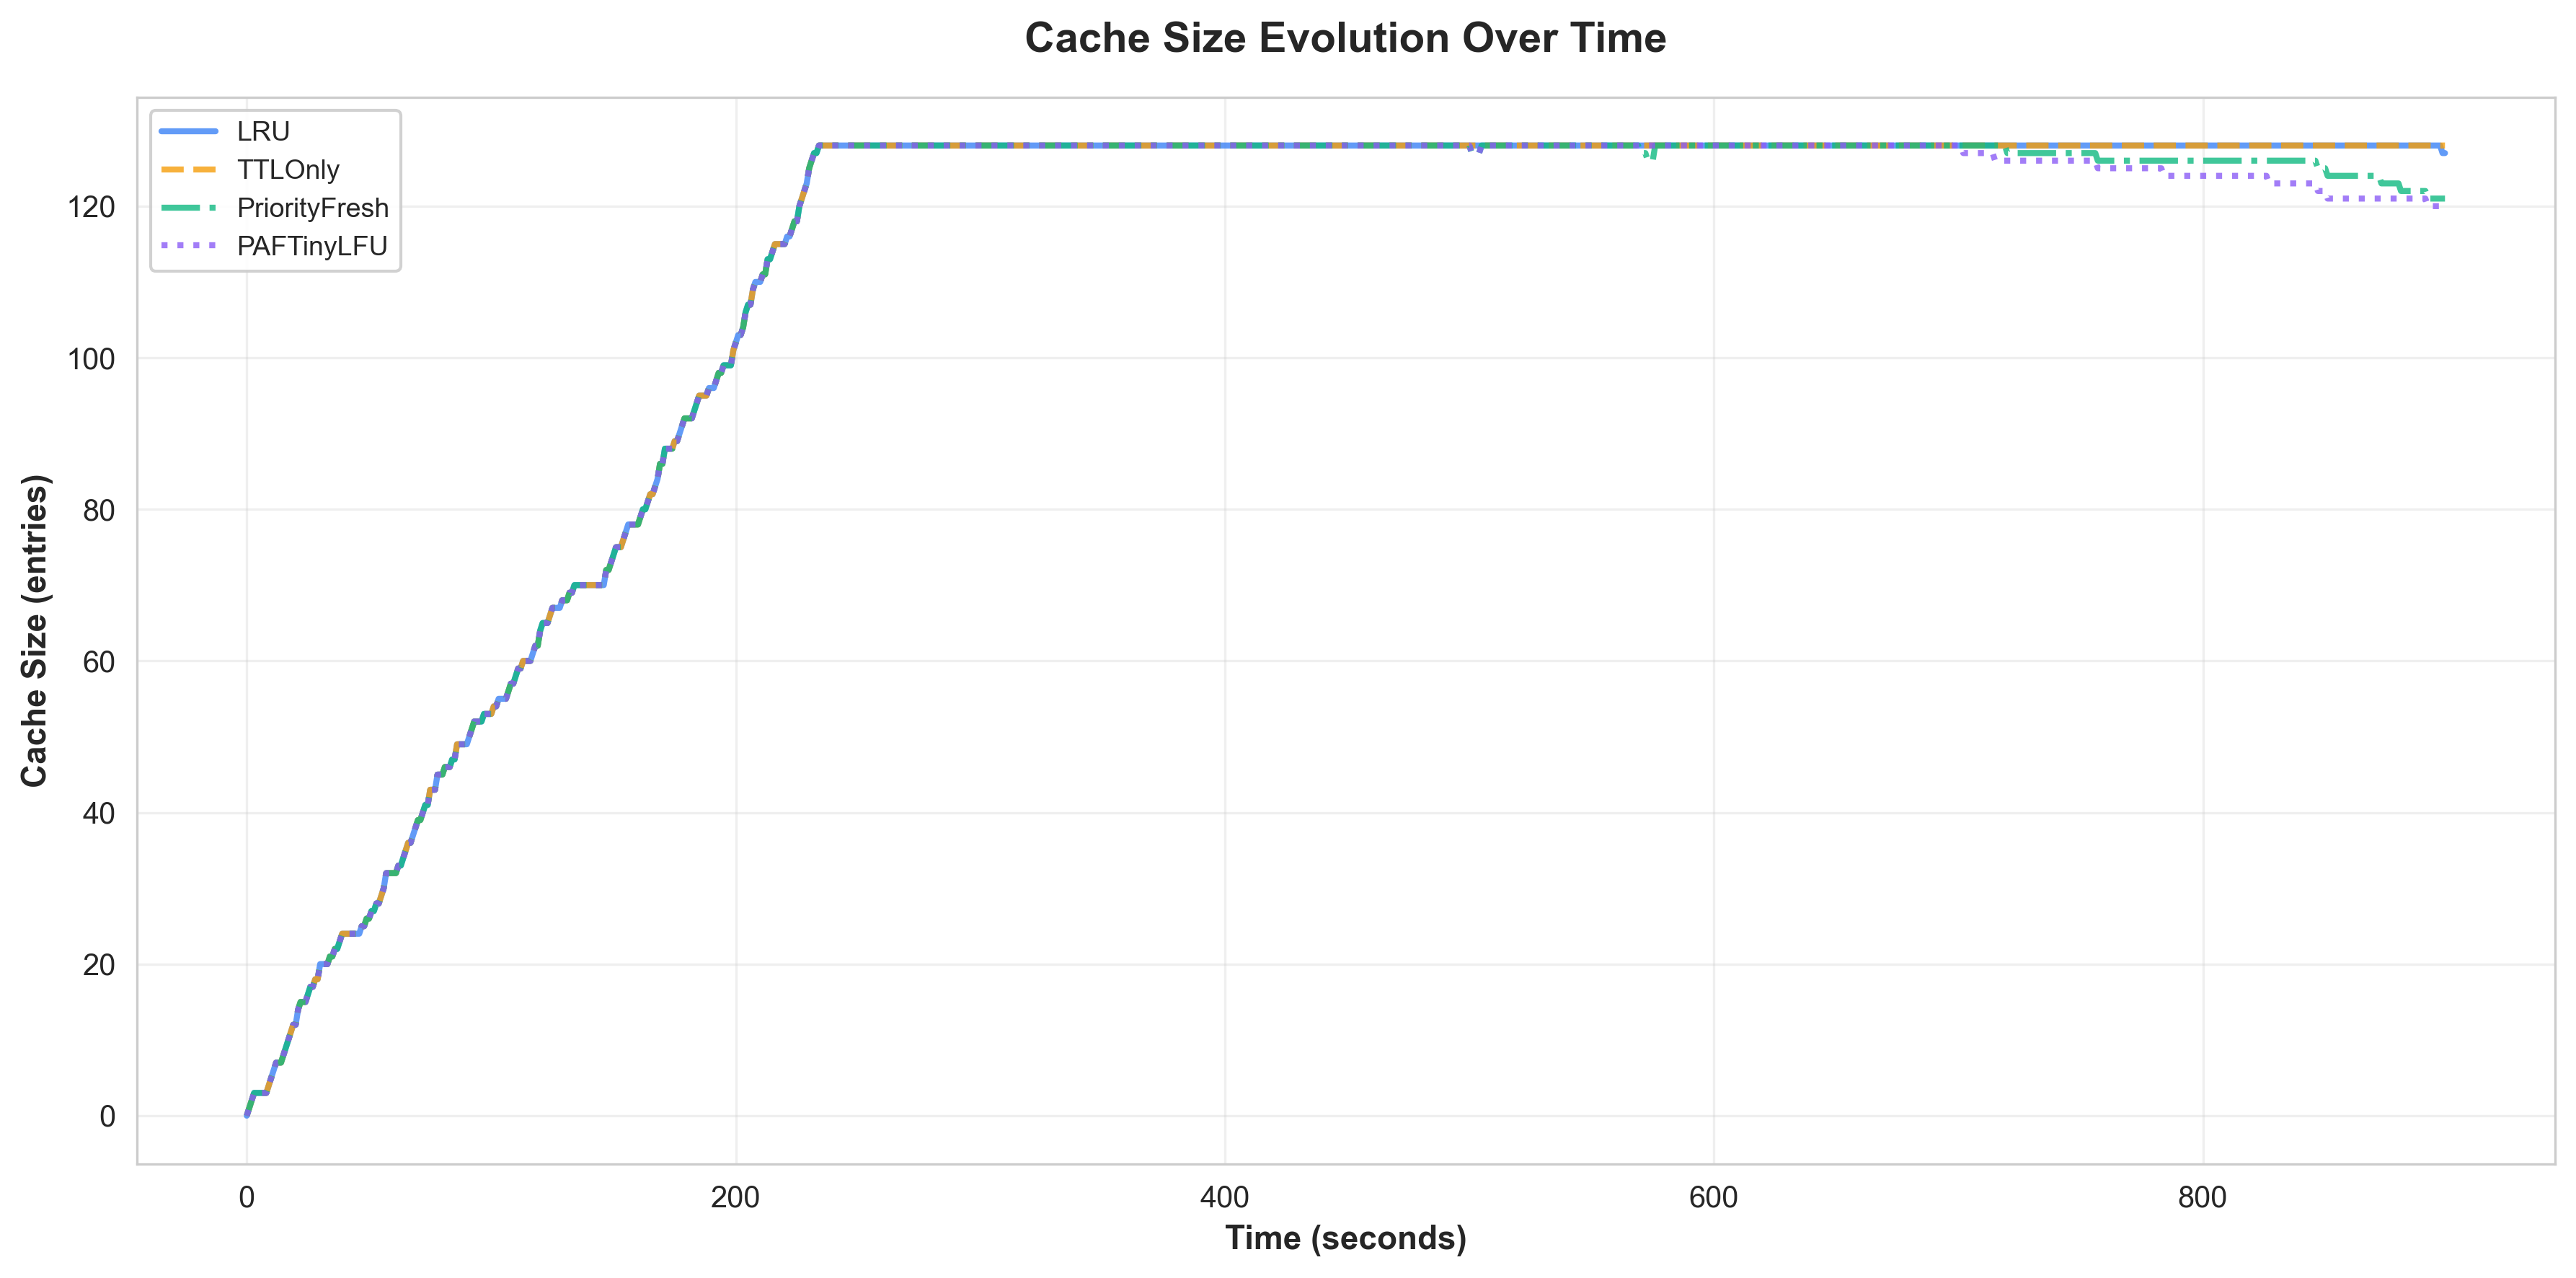
\includegraphics[width=\linewidth]{figures/timeline_cache_size_timeline.png}
    \caption{Cache size timeline under the baseline configuration.}
    \label{fig:timeline-cache-size}
\end{figure}

\vspace{0.2cm}
\vspace{0.2cm}

\section{Results and Analysis}
We now summarize quantitative findings from the CSV outputs in \texttt{scripts/data}. Unless noted, all runs use the default configuration in Table~\ref{tab:default-config}. Pushes were disabled (rate limit $R{=}0$), so delivery is governed solely by network reliability and cache behavior.

\subsection{Baseline (single seed)}
All four policies achieved nearly identical system efficiency under the baseline seed: cache hit rate $\approx 0.998$ and delivery rate $\approx 0.998$. Differences emerge in human-centered metrics:

\begin{table}[h]
\centering
\caption{Baseline metrics by policy (single-seed Urban, $C{=}128$, $\rho{=}0.85$)}
\label{tab:baseline-metrics}
\begin{tabular}{@{}lccccc@{}}
    \toprule
Policy & Hit & Deliver & Fresh & Actionable-1st & Time Cons. \\
\midrule
LRU & 0.998 & 0.998 & 0.843 & 0.850 & 0.211 \\
TTLOnly & 0.998 & 0.998 & \textbf{0.867} & 0.803 & 0.184 \\
PriorityFresh & 0.998 & 0.998 & 0.799 & \textbf{0.929} & 0.248 \\
PAFTinyLFU & 0.998 & 0.998 & 0.804 & 0.863 & \textbf{0.350} \\
\bottomrule
\end{tabular}
\end{table}

\noindent Observations (supported by Fig.~\ref{fig:baseline-grouped} and Fig.~\ref{fig:baseline-radar}):
\begin{itemize}
    \item \textbf{Actionability-first.} PriorityFresh leads on the fraction of threads where the first surfaced item is actionable, reflecting its semantic priority and PF-driven bias.
    \item \textbf{Freshness.} TTLOnly yields the freshest content (as expected from a TTL policy). PriorityFresh trades a small amount of freshness for actionability-first.
    \item \textbf{Timeliness consistency.} PAFTinyLFU stabilizes first-push timeliness the most; PriorityFresh improves over LRU/TTL but generally trails PAFTinyLFU on this metric.
\end{itemize}

\subsection{Cache-size scaling (device profiles)}
From \texttt{device-comparison-*.csv} and Fig.~\ref{fig:device-scaling-cachehit}--\ref{fig:device-all-grid}:
\begin{itemize}
    \item \textbf{Small caches (e.g., 32 entries, Budget Phone).} PriorityFresh maintains the highest actionability-first ratio ($\approx$0.97) and the highest timeliness consistency in this tier, while TTLOnly/LRU exhibit higher average freshness.
    \item \textbf{Moderate caches (128--256).} PriorityFresh continues to lead on actionability-first; PAFTinyLFU often edges out on timeliness consistency; freshness ordering remains TTLOnly $>$ LRU $>$ PriorityFresh $\approx$ PAFTinyLFU.
    \item \textbf{Large caches (512+).} Policies converge across all reported metrics—capacity is sufficient to retain most alerts, making selection effects negligible.
\end{itemize}

\subsection{Network reliability sweep}
From \texttt{network-comparison-*.csv} and Fig.~\ref{fig:network-delivery}--\ref{fig:network-all-grid}:
\begin{itemize}
    \item \textbf{Delivery rate tracks reliability uniformly.} With pushes disabled, all policies share essentially identical delivery under a given baseline reliability.
    \item \textbf{PriorityFresh sustains actionability-first across regimes.} The advantage in actionability-first holds from Perfect to Disaster networks.
    \item \textbf{Timeliness consistency.} PAFTinyLFU frequently attains the highest timeliness consistency, especially in mid-range reliabilities; PriorityFresh remains competitive and above LRU/TTL.
\end{itemize}

\subsection{Joint sweep (cache size \& network)}
From \texttt{combined-comparison-*.csv} and Fig.~\ref{fig:combined-heatmap-delivery}--\ref{fig:combined-reco-tree}:
\begin{itemize}
    \item \textbf{Monotonic surfaces.} Delivery rises with network reliability and shows diminishing returns with larger caches.
    \item \textbf{Where policies differ.} PriorityFresh wins actionability-first across most of the grid except in high-capacity regions where all policies tie; TTLOnly leads freshness; PAFTinyLFU often wins timeliness consistency.
\end{itemize}

\subsection{Timeline behavior}
The per-run timelines (Fig.~\ref{fig:timeline-dashboard}, \ref{fig:timeline-hitrate}--\ref{fig:timeline-cache-size}) show smooth convergence of hit rate to $\sim$0.998 for all policies under the baseline seed, consistent with the point-in-time summaries.

\paragraph{Takeaways.}
PriorityFresh preserves system efficiency while consistently improving the actionability of what users see first, particularly when cache is constrained or networks are degraded. TTLOnly is a strong baseline for freshness; PAFTinyLFU provides the most stable first-push timing. In practice, PriorityFresh can be paired with a PF threshold tuned to operator goals: higher $\tau$ for stricter actionability-first, lower $\tau$ if freshness is paramount.

\subsection{Answering the research question}
\label{sec:rq-answer}
Our results indicate that the most effective way to deliver the most pressing matters is to \emph{optimize what surfaces first} rather than maximizing total coverage. PriorityFresh is designed for this exact objective:
\begin{itemize}
    \item \textbf{Actionability-first by construction.} The scoring emphasizes urgency, severity, and recency; the PF boost can tilt toward historically high-value patterns. This yields the top actionability-first ratio across regimes.
    \item \textbf{Hold until no longer relevant.} Decay and expiry remove items once they are no longer pressing. This maintains focus on ongoing, high-impact threads instead of churning through the catalog.
    \item \textbf{Tradeoffs are intentional.} PriorityFresh is \emph{not} a mass-coverage model. Its average freshness and timeliness stability reflect a conscious trade to ensure the right items show up first. TTLOnly leads in average freshness; PAFTinyLFU stabilizes timing—both are compatible fallbacks when those criteria are primary.
    \item \textbf{Operator levers.} Weights $(w_S,w_U,w_F)$ and PF threshold $\tau$ act as knobs: increase $w_U$/$w_S$ or $\tau$ when “pressing matters” should be filtered aggressively; relax them when broader recall or freshness is preferred.
    \item \textbf{Push discipline (when enabled).} Rate limits and deduplication suppress redundant pings. With PF-enabled pushes, the same actionability-first principle governs \emph{which} threads break through to notifications rather than “spitting out” many alerts.
\end{itemize}

Put simply, if the research question is about surfacing what matters most, the evaluation shows PriorityFresh answers it: it consistently leads on actionability-first without sacrificing system efficiency, and it provides explicit controls to tune how aggressively “pressing” is interpreted for different operational contexts.

\vspace{0.2cm}
\noindent\textit{Note.} Non-essential system, evaluation, and background sections have been moved to a companion file for future use.

\FloatBarrier
\clearpage
\begin{thebibliography}{99}

\bibitem{oasis-cap-1.2}
OASIS, ``Common Alerting Protocol (CAP) Version 1.2,'' OASIS Standard, Jul.\ 1, 2010. Available: \url{https://docs.oasis-open.org/emergency/cap/v1.2/CAP-v1.2-os.html}

\bibitem{fcc-2018-geo}
Federal Communications Commission, ``Wireless Emergency Alerts; Emergency Alert System,'' \emph{Federal Register}, 83(40), Feb.\ 28, 2018. (Defines matching the target area with no more than 0.1\,mile overshoot.) Available: \url{https://www.federalregister.gov/documents/2018/02/28/2018-03990/wireless-emergency-alerts-emergency-alert-system}

\bibitem{fcc-wea-2023-doc}
Federal Communications Commission, ``Wireless Emergency Alerts; Emergency Alert System,'' \emph{Federal Register}, 88(118), pp.\ 40166--40188, Jun.\ 21, 2023. (Codifies 0.1\,mile accuracy, transmission speed requirements.) Available: \url{https://www.federalregister.gov/documents/2023/06/21/2023-12725/wireless-emergency-alerts-emergency-alert-system}

\bibitem{rand-wea-2023-test}
A.\ M.\ Parker \emph{et al.}, ``Assessing Public Reach of the 2023 National Test of the Wireless Emergency Alerts (WEA) System: Results of a National Survey,'' RAND/HSOAC Research Report RR-A2451-1, 2024. Available: \url{https://www.rand.org/pubs/research_reports/RRA2451-1.html}

\bibitem{mcbride-2023-wea-latency}
S.\ K.\ McBride, R.\ Allen, S.\ Baltay, \emph{et al.}, ``Latency and geofence testing of Wireless Emergency Alerts for ShakeAlert,'' \emph{Safety Science}, vol.\ 157, 2023, Art.\ 105999. doi:\,10.1016/j.ssci.2022.105999

\bibitem{kleppmann-2019-localfirst}
M.\ Kleppmann, A.\ Wiggins, N.\ Zeldovich, ``Local-First Software: You Own Your Data, in spite of the Cloud,'' \emph{Onward! 2019}, pp.\ 154--178. doi:\,10.1145/3359591.3359737

\bibitem{mec-caching-survey-2023}
T.\ V.\ Nguyen, A.\ T.\ Tran, N.\ N.\ Dao, H.\ Moon, S.\ Cho, ``Information fusion on delivery: A survey on the roles of mobile edge caching systems,'' \emph{Information Fusion}, vol.\ 89, pp.\ 486--509, Jan.\ 2023. doi:\,10.1016/j.inffus.2022.08.029

\bibitem{icn-iot-caching-survey-2023}
C.\ N.\ Pruthvi, H.\ S.\ Vimala, J.\ Shreyas, ``A systematic survey on content caching in ICN and ICN-IoT: Challenges, approaches and strategies,'' \emph{Computer Networks}, vol.\ 233, 2023, Art.\ 109896. doi:\,10.1016/j.comnet.2023.109896

\bibitem{cache-mab-2023}
S.\ M.\ A.\ Iqbal, M.\ Asaduzzaman, ``Cache-MAB: A reinforcement learning–based hybrid caching scheme in Named Data Networks,'' \emph{Future Generation Computer Systems}, vol.\ 147, pp.\ 163--178, 2023. doi:\,10.1016/j.future.2023.04.032

\bibitem{electronics-2024-koide-icanet}
M.\ Koide, Y.\ Ohira, Y.\ Hirota, ``Caching for Information-Centric Ad Hoc Networks using Popularity and Node Centrality,'' \emph{Electronics}, vol.\ 13, no.\ 11, 2024, Art.\ 2213. doi:\,10.3390/electronics13112213

\bibitem{hotnets-2024-freshness}
Z.\ Mao, R.\ Iyer, S.\ Shenker, I.\ Stoica, ``Revisiting Cache Freshness for Emerging Real-Time Applications,'' in \emph{Proc.\ ACM HotNets 2024}. doi:\,10.1145/3696348.3696858

\bibitem{einziger-2017-wtinylfu}
G. Einziger, R. Friedman, ``TinyLFU: A Highly Efficient Cache Admission Policy,'' \emph{IEEE Trans. on Knowledge and Data Engineering}, vol. 29, no. 4, pp. 826--841, 2017. doi:\,10.1109/TKDE.2016.2632726

\bibitem{shevchenko-2023-geofencing}
V.\ Shevchenko, M.\ Rabinovich, A.\ Shoval, \emph{et al.}, ``Geofencing in location-based behavioral research,'' \emph{Behavior Research Methods}, 2024. doi:\,10.3758/s13428-024-02440-3

\bibitem{mileti-1990-ornl6609}
D.\ S.\ Mileti, J.\ H.\ Sorensen, ``Communication of Emergency Public Warnings: A Social Science Perspective and State-of-the-Art Assessment,'' Oak Ridge National Laboratory Report ORNL-6609, Aug.\ 1990. doi:\,10.2172/6137387

\bibitem{cohen-1985-socialsupport}
S.\ Cohen, T.\ A.\ Wills, ``Stress, social support, and the buffering hypothesis,'' \emph{Psychological Bulletin}, vol.\ 98, no.\ 2, pp.\ 310--357, 1985.

\bibitem{norris-2008-resilience}
F.\ H.\ Norris, S.\ P.\ Stevens, B.\ Pfefferbaum, K.\ F.\ Wyche, R.\ L.\ Pfefferbaum, ``Community Resilience as a Metaphor, Theory, Set of Capacities, and Strategy for Disaster Readiness,'' \emph{American Journal of Community Psychology}, vol.\ 41, pp.\ 127--150, 2008. doi:\,10.1007/s10464-007-9156-6

\bibitem{paton-2008-warningresponse}
D.\ Paton, ``Risk communication and natural hazard mitigation: How trust influences its effectiveness,'' \emph{International Journal of Global Environmental Issues}, vol.\ 8, nos.\ 1--2, pp.\ 2--16, 2008. doi:\,10.1504/IJGENVI.2008.017256

\bibitem{nasem-2018-alerts}
National Academies of Sciences, Engineering, and Medicine, ``Emergency Alert and Warning Systems: Current Knowledge and Future Research Needs,'' Washington, DC: The National Academies Press, 2018. doi:\,10.17226/24935

\bibitem{lindell-2012-padm}
M.\ K.\ Lindell, R.\ W.\ Perry, ``The Protective Action Decision Model: Theoretical Modifications and Additional Evidence,'' \emph{Risk Analysis}, vol.\ 32, no.\ 4, pp.\ 616--632, 2012. doi:\,10.1111/j.1539-6924.2011.01647.x

\end{thebibliography}


\end{document}